\documentclass{article}
\usepackage{ctex,amsmath,tcolorbox,tikz,extarrows,lastpage,fancyhdr,amssymb,amsthm,framed,graphicx,changepage,mathrsfs,booktabs,bbding,tikz,listings,siunitx,pdfpages}
\usepackage[colorlinks,
linkcolor=blue,
anchorcolor=blue,
urlcolor=blue,
citecolor=blue]{hyperref}
\usepackage{cleveref}
\tcbuselibrary{most}
\usepackage{xcolor}
\usepackage{listings}
%-------------------------------
\usepackage{geometry}
\usepackage{caption}
\captionsetup[figure]{labelfont={bf},labelformat={default},labelsep=period,name={Fig }}
\geometry{a4paper,left=25mm,right=25mm,top=25mm,bottom=25mm}
\captionsetup[table]{labelfont={bf},labelformat={default},labelsep=period,name={Tab }}
\geometry{a4paper,left=25mm,right=25mm,top=25mm,bottom=25mm}
%-------------------------------
\newdimen\doublelineskip 
\setlength\doublelineskip{2pt}
\setlength\headheight{21pt}

\fancypagestyle{doubleline}{
	\renewcommand\headrule{
		\hrule height\headrulewidth width\headwidth
		\vskip \doublelineskip
		\hrule height\headrulewidth width\headwidth}
}
	\usepackage{booktabs}  
\usepackage{multirow}  
\usepackage{adjustbox} 
\definecolor{emphasis}{HTML}{780206}
\definecolor{newgreen}{HTML}{237A57}
\definecolor{newblue}{HTML}{155799}
\renewcommand{\thefootnote}{*}
\renewcommand{\contentsname}{Contents}
\renewcommand{\refname}{References}
%----------------------------------
\usepackage{listings}
\usepackage{xcolor}
\lstset{tabsize=4, 
	frame=shadowbox, 
	commentstyle=\color{red!50!green!50!blue!50},
	rulesepcolor=\color{red!20!green!20!blue!20},
	keywordstyle=\color{blue!90}\bfseries, 
	showstringspaces=false,
	stringstyle=\ttfamily, 
	keepspaces=true, 
	breakindent=22pt, 
	numbers=left,
	stepnumber=1,
	numberstyle=\tiny, 
	basicstyle=\footnotesize, 
	showspaces=false, 
	flexiblecolumns=true, 
	breaklines=true, 
	breakautoindent=true,
	breakindent=4em, 
	escapebegin=\begin{CJK*}{GBK}{hei},escapeend=\end{CJK*},
	aboveskip=1em, 
	fontadjust,
	captionpos=t,
	framextopmargin=2pt,framexbottommargin=2pt,abovecaptionskip=-3pt,belowcaptionskip=3pt,
	xleftmargin=4em,xrightmargin=4em, 
	texcl=true,
	extendedchars=false,columns=flexible,mathescape=true
}

%--------------------------------
\title{STA 141A Winter 2025 Final Project:\\
	From Neural Dynamics to Behavior: Predictive Modeling of Visual Decision Outcomes}
\author{919257083\qquad Yunze Hang}
\date{}
\begin{document}
	\maketitle
	\begin{figure}[htbp]
		\centering
		
\includegraphics[scale = 0.5]{Pics/1}
		\label{fig:1}
	\end{figure}
	$${\centering{\mbox{\date{Wednesday, March 12th, 2025}}}}$$
	\clearpage
	\setcounter{page}{1}
	\pagenumbering{Roman}
	\tableofcontents
	\clearpage
	\fancyhead[L]{Yunze Hang}
	\fancyhead[R]{}
	\pagenumbering{arabic}
	\pagestyle{doubleline}
	\cfoot{\thepage / \pageref{LastPage}}
	\section{Abstract}
	\par Nowadays, as the development of brain-machine interfaces and other new devices in the field of modern neuroscience, the ability to decode behavioral outcomes from neural activity becomes an important cornerstone. This project studies a subset of data from ``\textit{Distributed coding of choice, action and engagement across the mouse brain}" by Steinmetz et al. (2019)\cite{ref1} in the field of perceptual decision, mainly focusing on $18$ experimental sessions across $4$ mice performing a visual contrast discrimination task.
	\par During these $18$ sessions, $4$ mice were presented with bilateral visual stimuli of varying contrasts and rewarded for correctly indicating the side of higher contrast (or do nothing when in zero-contrast situations). Neural activities from the visual cortex was recorded by Neuropixels probes as spike trains, providing a high-dimensional dataset to explore the relationship between sensory input, neural dynamics, and behavioral outcomes.
	\par The main objective is to develop a predictive model that integrates neural activities across $0$ to $0.4$s and stimulus contrasts to classify trail outcomes. (Success for $1$, Failure for $0.$) To address the goal, we structure our statistical analysis into the following several procedures:
	\begin{itemize}
		\item [1)] \textbf{Introduction to the experiment}
		\item [2)] \textbf{Exploratory data analysis}
		\item [3)] \textbf{Data integration}
		\item [4)] \textbf{Model training and prediction}
	\end{itemize}
	\par In the Data integration part, we used PCA to reduce the high dimensional data; In the Model training and prediction part, we applied many different kinds of predictive models including LASSO, KNN, Logistic Regression, XGBoost, with SMOTE. Moreover, we learnt from the reference\cite{ref1} and found a new statistical method with Kernel Functions.
	\par This work not only advances methodological frameworks for analyzing high-dimensional and large-scale neural datasets but also contributes to understanding how visual cortex activity encodes perceptual decision.
	\par \textbf{Key Words}
	\begin{itemize}
		\item Neuroscience
		\item Perceptual Decision
		\item PCA
		\item Harmony Algorithm
		\item LASSO
		\item KNN
		\item Logistic Regression
		\item SMOTE
		\item XGBoost
	\end{itemize}
	\clearpage
	\section{Introduction to the Experiment}
	\par The experiment analyzed in this study investigates the neural correlations of perceptual decision in mice by doing a visual contrast discrimination task, originally designed by Steinmetz et al. (2019)\cite{ref1}.
	\par On each trial, visual stimuli of varying contrast $(0, 0.25, 0.5, \mbox{or} 1)$ could appear on the left side, right side, both sides or neither side. Mice earned a water reward by turning a wheel with their forepaws to indicate which side had highest contrast (Fig.\ref{fig:001}). If neither stimulus was present, they earned a reward for making a third type of response: keeping the wheel still for $1.5$s. If left and right stimuli had equal non-zero contrast, the mice were rewarded randomly for left or right turns.
	\begin{figure}[htbp]
		\centering
		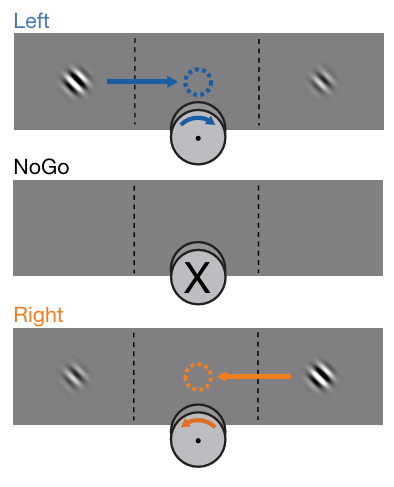
\includegraphics[scale = 0.7]{Pics/001}
		\caption{Mice earned water rewards by turning a wheel to indicate which of 
			two visual gratings had higher contrast, or by not turning if no stimulus was 
			presented. When stimuli had equal contrast, a left or right choice was rewarded 
			with 50\% probability. Grey rectangles indicate the three computer screens 
			surrounding the mouse. Arrows (not visible to the mouse) indicate the rewarded 
			wheel turn direction and the coupled movement of the visual stimulus (X 
			indicates reward for no turn), and the coloured dashed circle (not visible to the 
			mouse) indicates the stimulus location at which a reward was delivered.}
		\label{fig:001}
	\end{figure}
	\par The total data in ref\cite{ref1} was recorded by Neuropixels probes, with approximately 30,000 neurons in 42 brain regions of mice performing a visual discrimination task. 
	\begin{figure}[htbp]
		\centering
		\begin{minipage}[t]{0.48\textwidth}
			\centering
			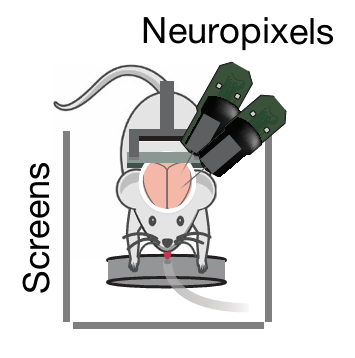
\includegraphics[scale=0.4]{Pics/Mouse}\label{fig:1.01}
			\caption{Mouse and the Neuropixels}
		\end{minipage}
		\begin{minipage}[t]{0.48\textwidth}
			\centering
			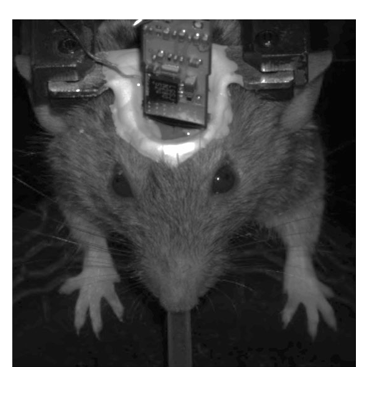
\includegraphics[scale=0.4]{Pics/Mouse2}\label{fig:1.02}
			\caption{The Picture in Real Experiment}
		\end{minipage}
	\end{figure}
	\clearpage
	\par Moreover, each session's data was a nested list has the following elements:
		\begin{framed}
		\begin{verbatim}
			names(sessions[[5]])
			'contrast_left' 'contrast_right' 'feedback_type' 'mouse_name' 'brain_area' 
			'date_exp' 'spks' 'time'
		\end{verbatim}
	\end{framed}
	\par Our main goal is to build up a predictive model for the outcomes ($1$ for success, $-1$ for failure). We'll start our task step by step, firstly exploring data, then reducing the dimension, finally training our models and finding the most optimal one (model selection).
	\section{Exploratory Data Analysis}
	\par In this part, we will explore the features of the data sets in order to build our prediction model. 
	\subsection{Data Structures across Sessions}
	\subsubsection{Number of Neurons and Number of Trials Each Session}
	\par Firstly, with the data on hand, we are curious about how many neurons and how many trials for each session. After coding, the visualized bar plot is shown below, where the blue bars represent the number of neurons for each session and the yellow ones represent the number of trials for each session. There are $18$ sessions in total, as we mentioned in the last section.
	\begin{figure}[htbp]
		\centering
		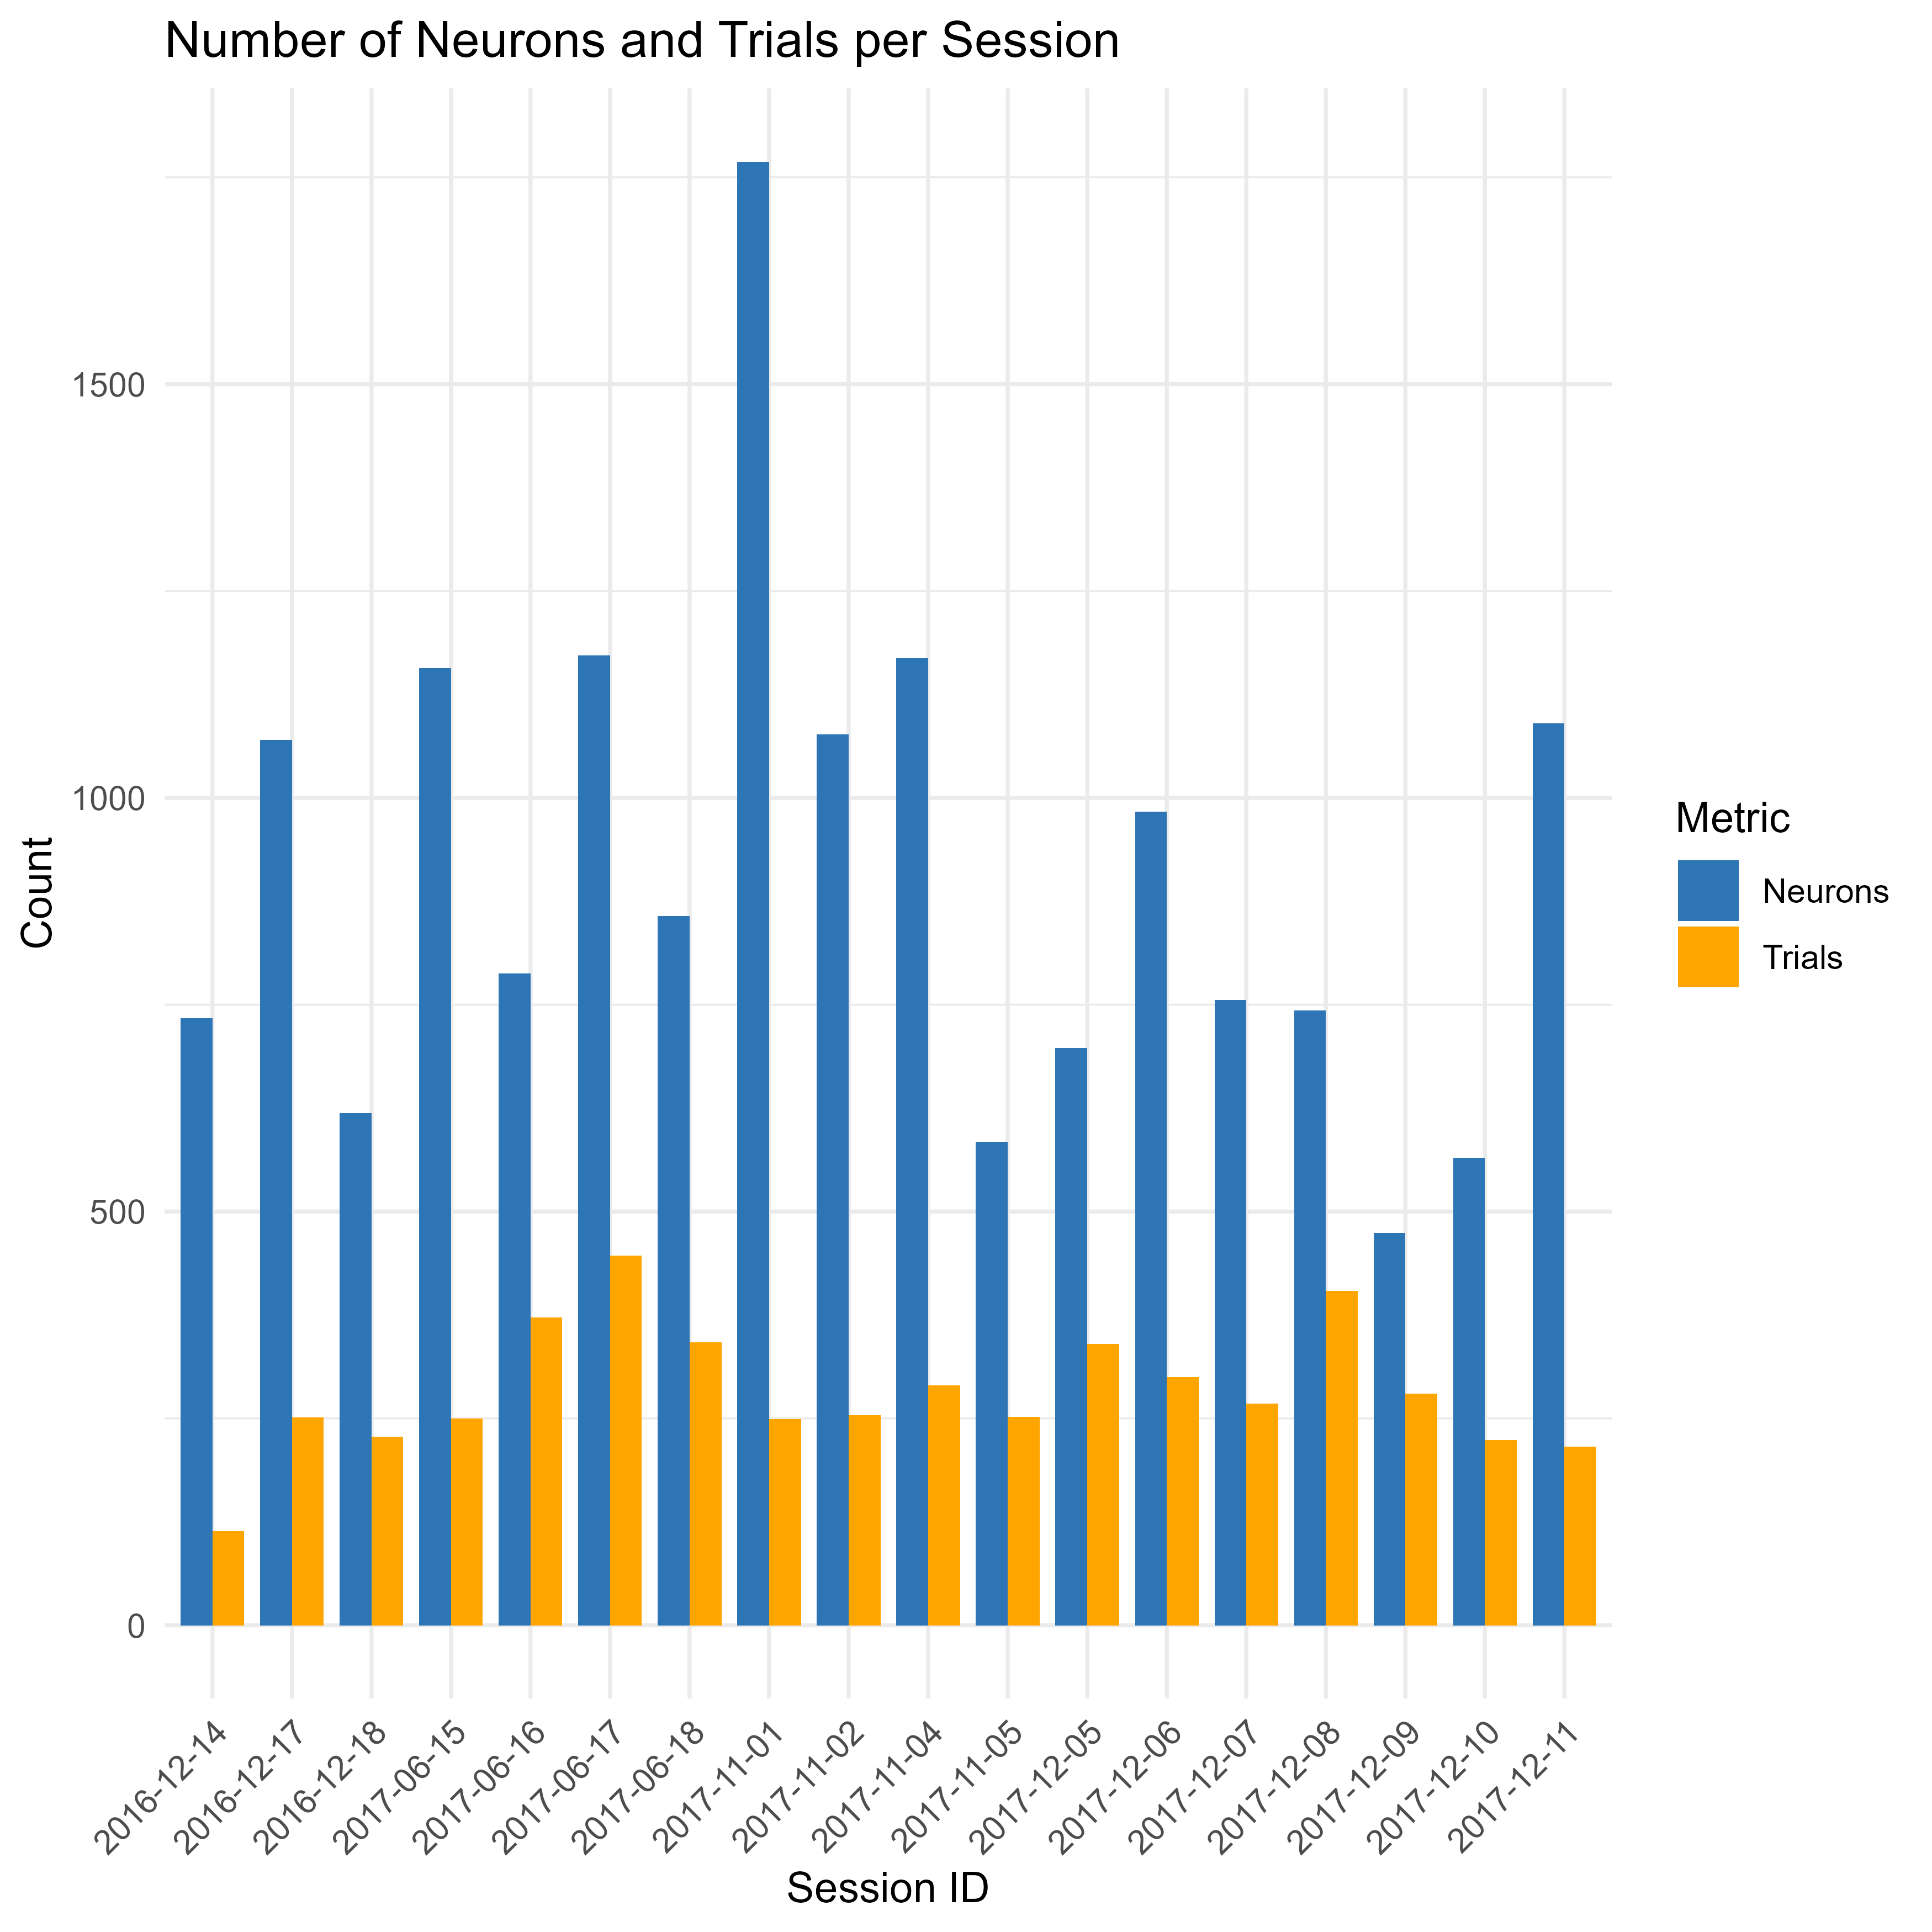
\includegraphics[scale = 0.5]{Pics/004}
		\caption{The Number of Neurons and the Number of Trials}
		\label{fig:004}
	\end{figure}
	\par The means for those statistics above are: $906$ for the number of Neurons and $282$ for the number of Trials over $18$ different sessions. Those numbers are enough for us to get a well performed predictive model. More details are shown in the table, see Appendix Table \ref{tab:session_summary}.
	\clearpage
	\subsubsection{The Distribution of Stimuli Conditions Across Sessions}
	\par The stimuli conditions are also presented by different $18$ heat maps as follows.
	\begin{figure}[htbp]
		\centering
		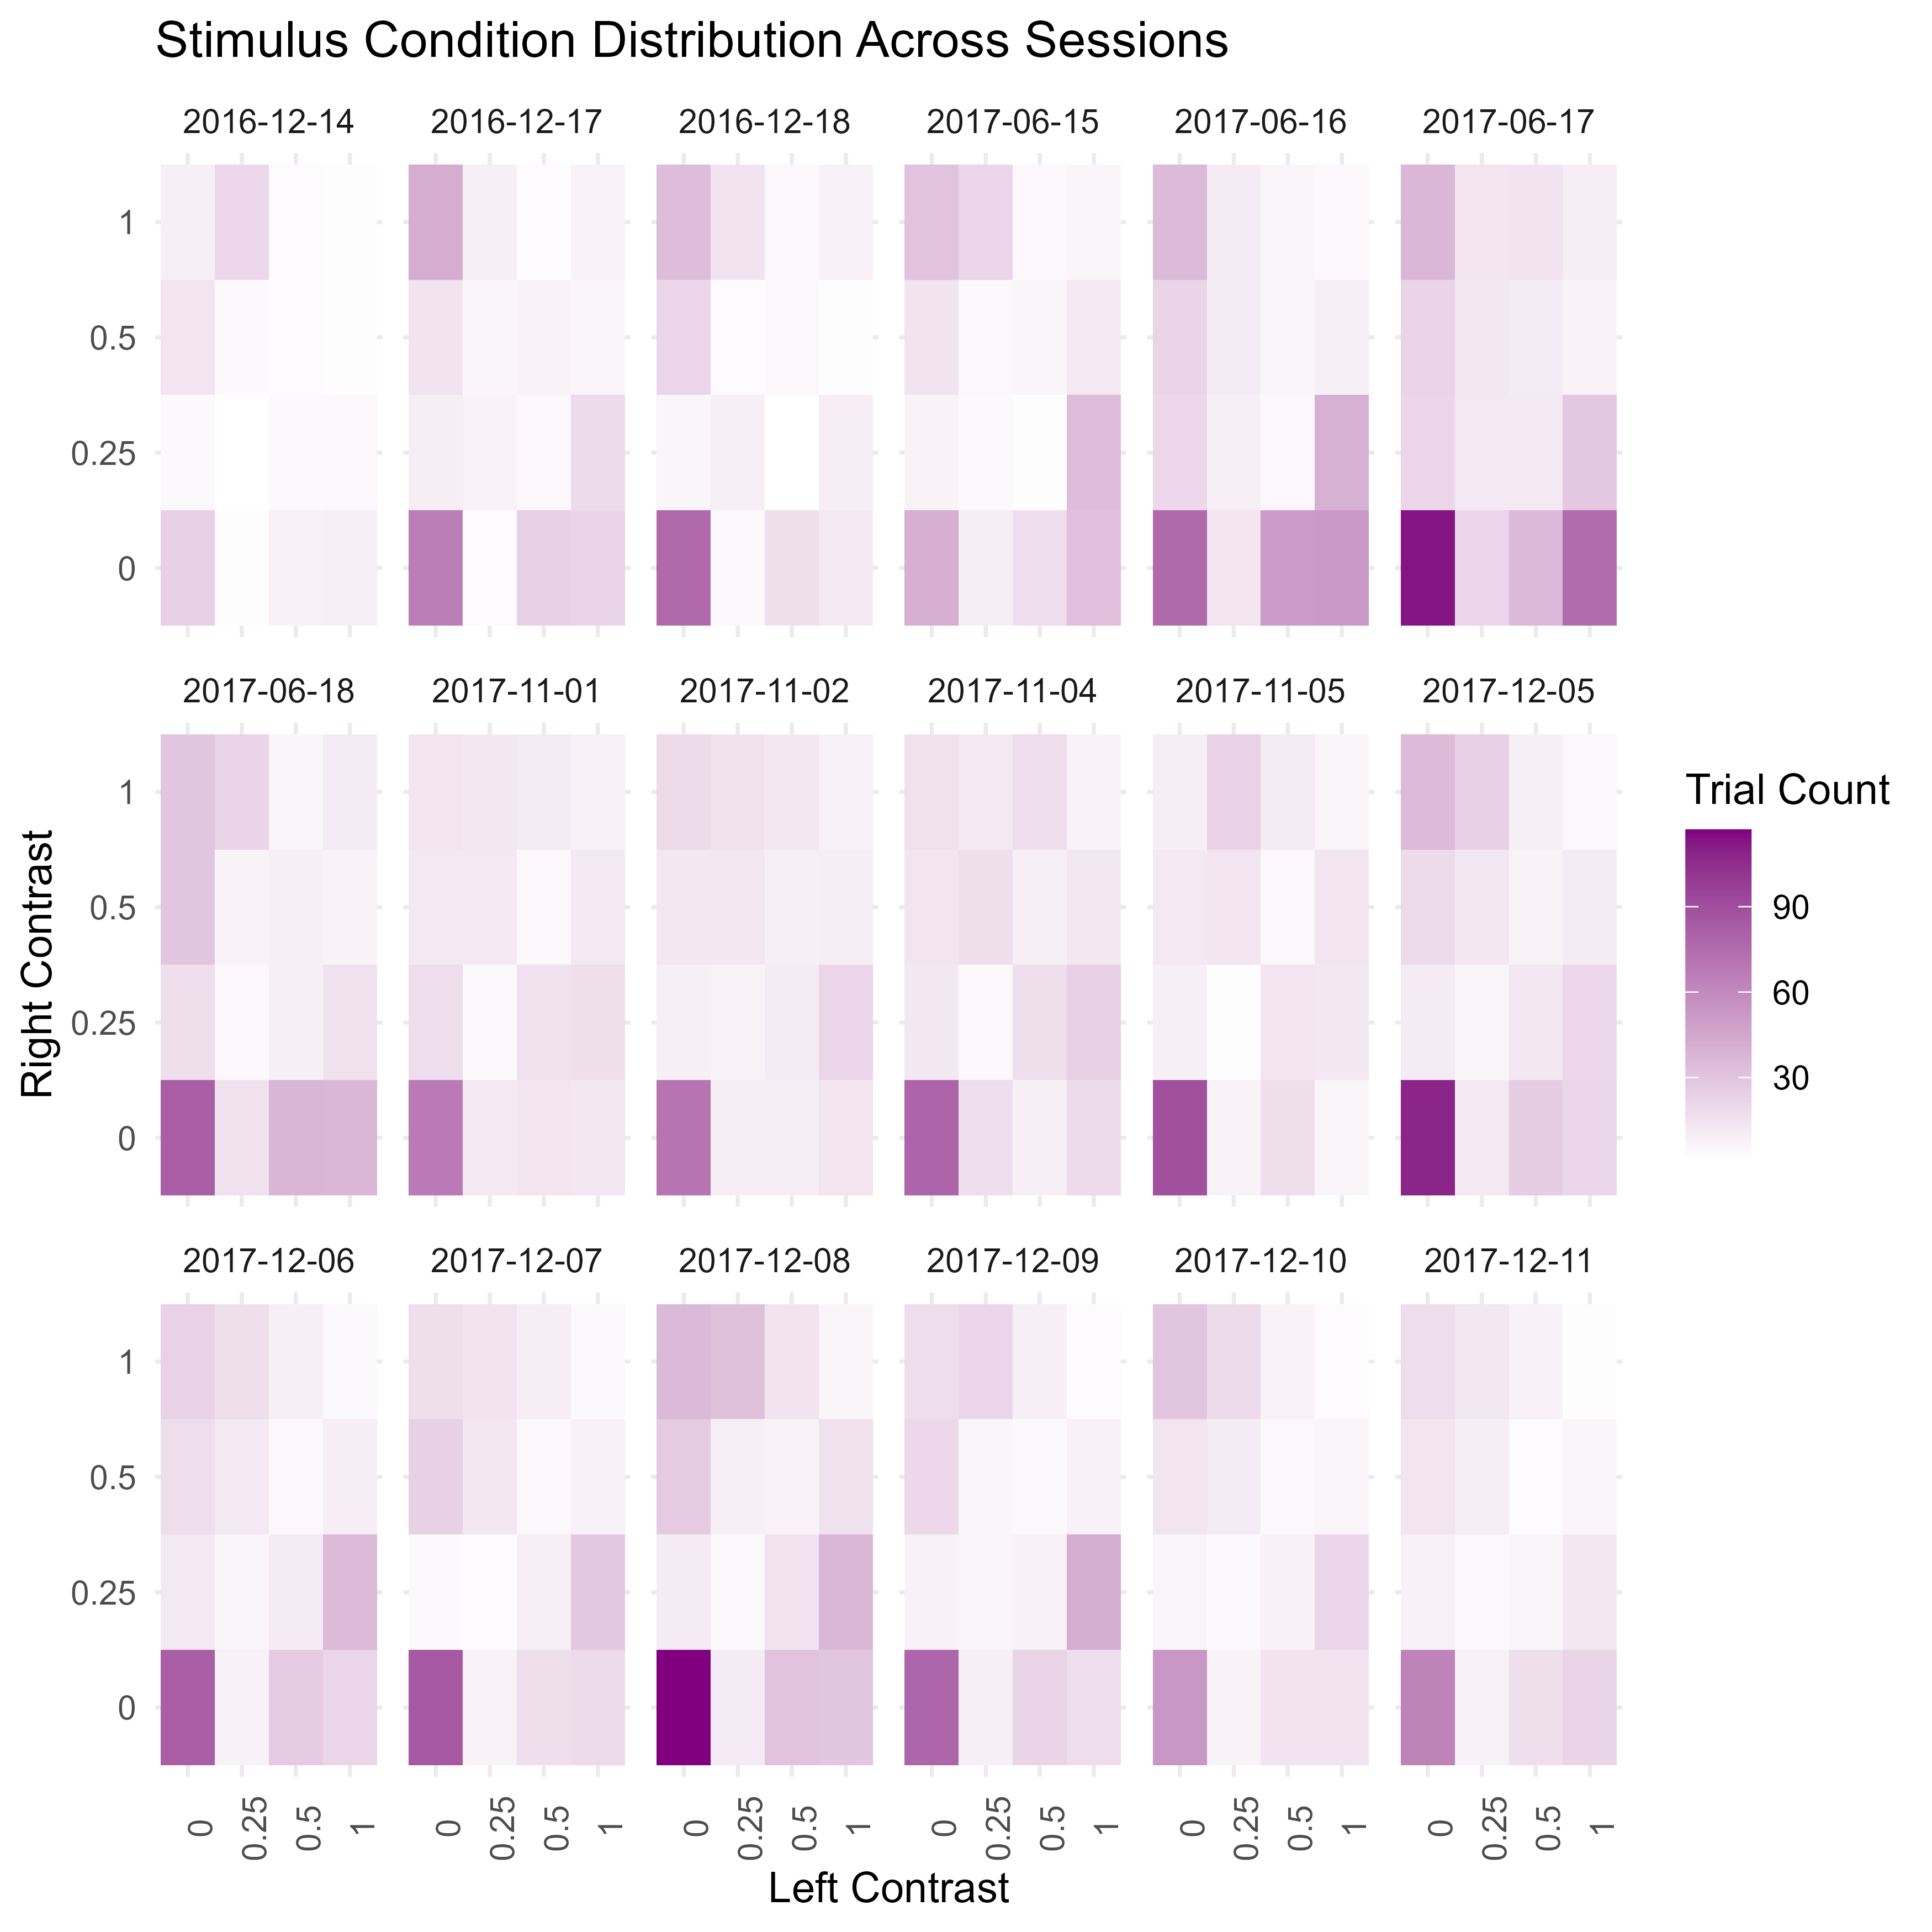
\includegraphics[scale = 0.7]{Pics/005}
		\caption{The Distribution of Stimuli Conditions Across Sessions}
		\label{fig:005}
	\end{figure}
	\par As we can see, the high frequency of trials with $(\mbox{contrast\_left, contrast\_right}) = (0,0)$ in the statistics is likely a deliberate feature of the experimental design. In the experiment, the $(0,0)$ condition, which means no signal on any screens, represents \textbf{a no-stimuli trial}, where is typically to test whether the mouse can correctly inhibit its behavior and reaction in the absence of sensory cues.
	\par It may serve the following propose:
	\begin{itemize}
		\item [1)] \textbf{Task Rule Learning:} By frequently presenting no-stimulus trials, the experiment tries its best to ensure that every mouse learns the rule of task instead of turning the wheel left or right randomly. It's fundamental for the experiment.
		\item [2)] \textbf{Distinguish from Random Moves:} With frequently no-stimulus trials, we can study the behavior of neurons when there's no stimuli.
		\item [3)] \textbf{Controlling the Difficulty:} Designing experiment with more no-stimulus trials help the tasks more easier to understand, ensuring that the mice do not develop bias towards always turning the wheel.
	\end{itemize}
	\clearpage
	\subsubsection{Feedback Types}
	\par As the experiment mentioned in the last section, there are two feedback types in total: Success and Failure. We plotted the pie chart for each session as follows.
	\begin{figure}[htbp]
		\centering
		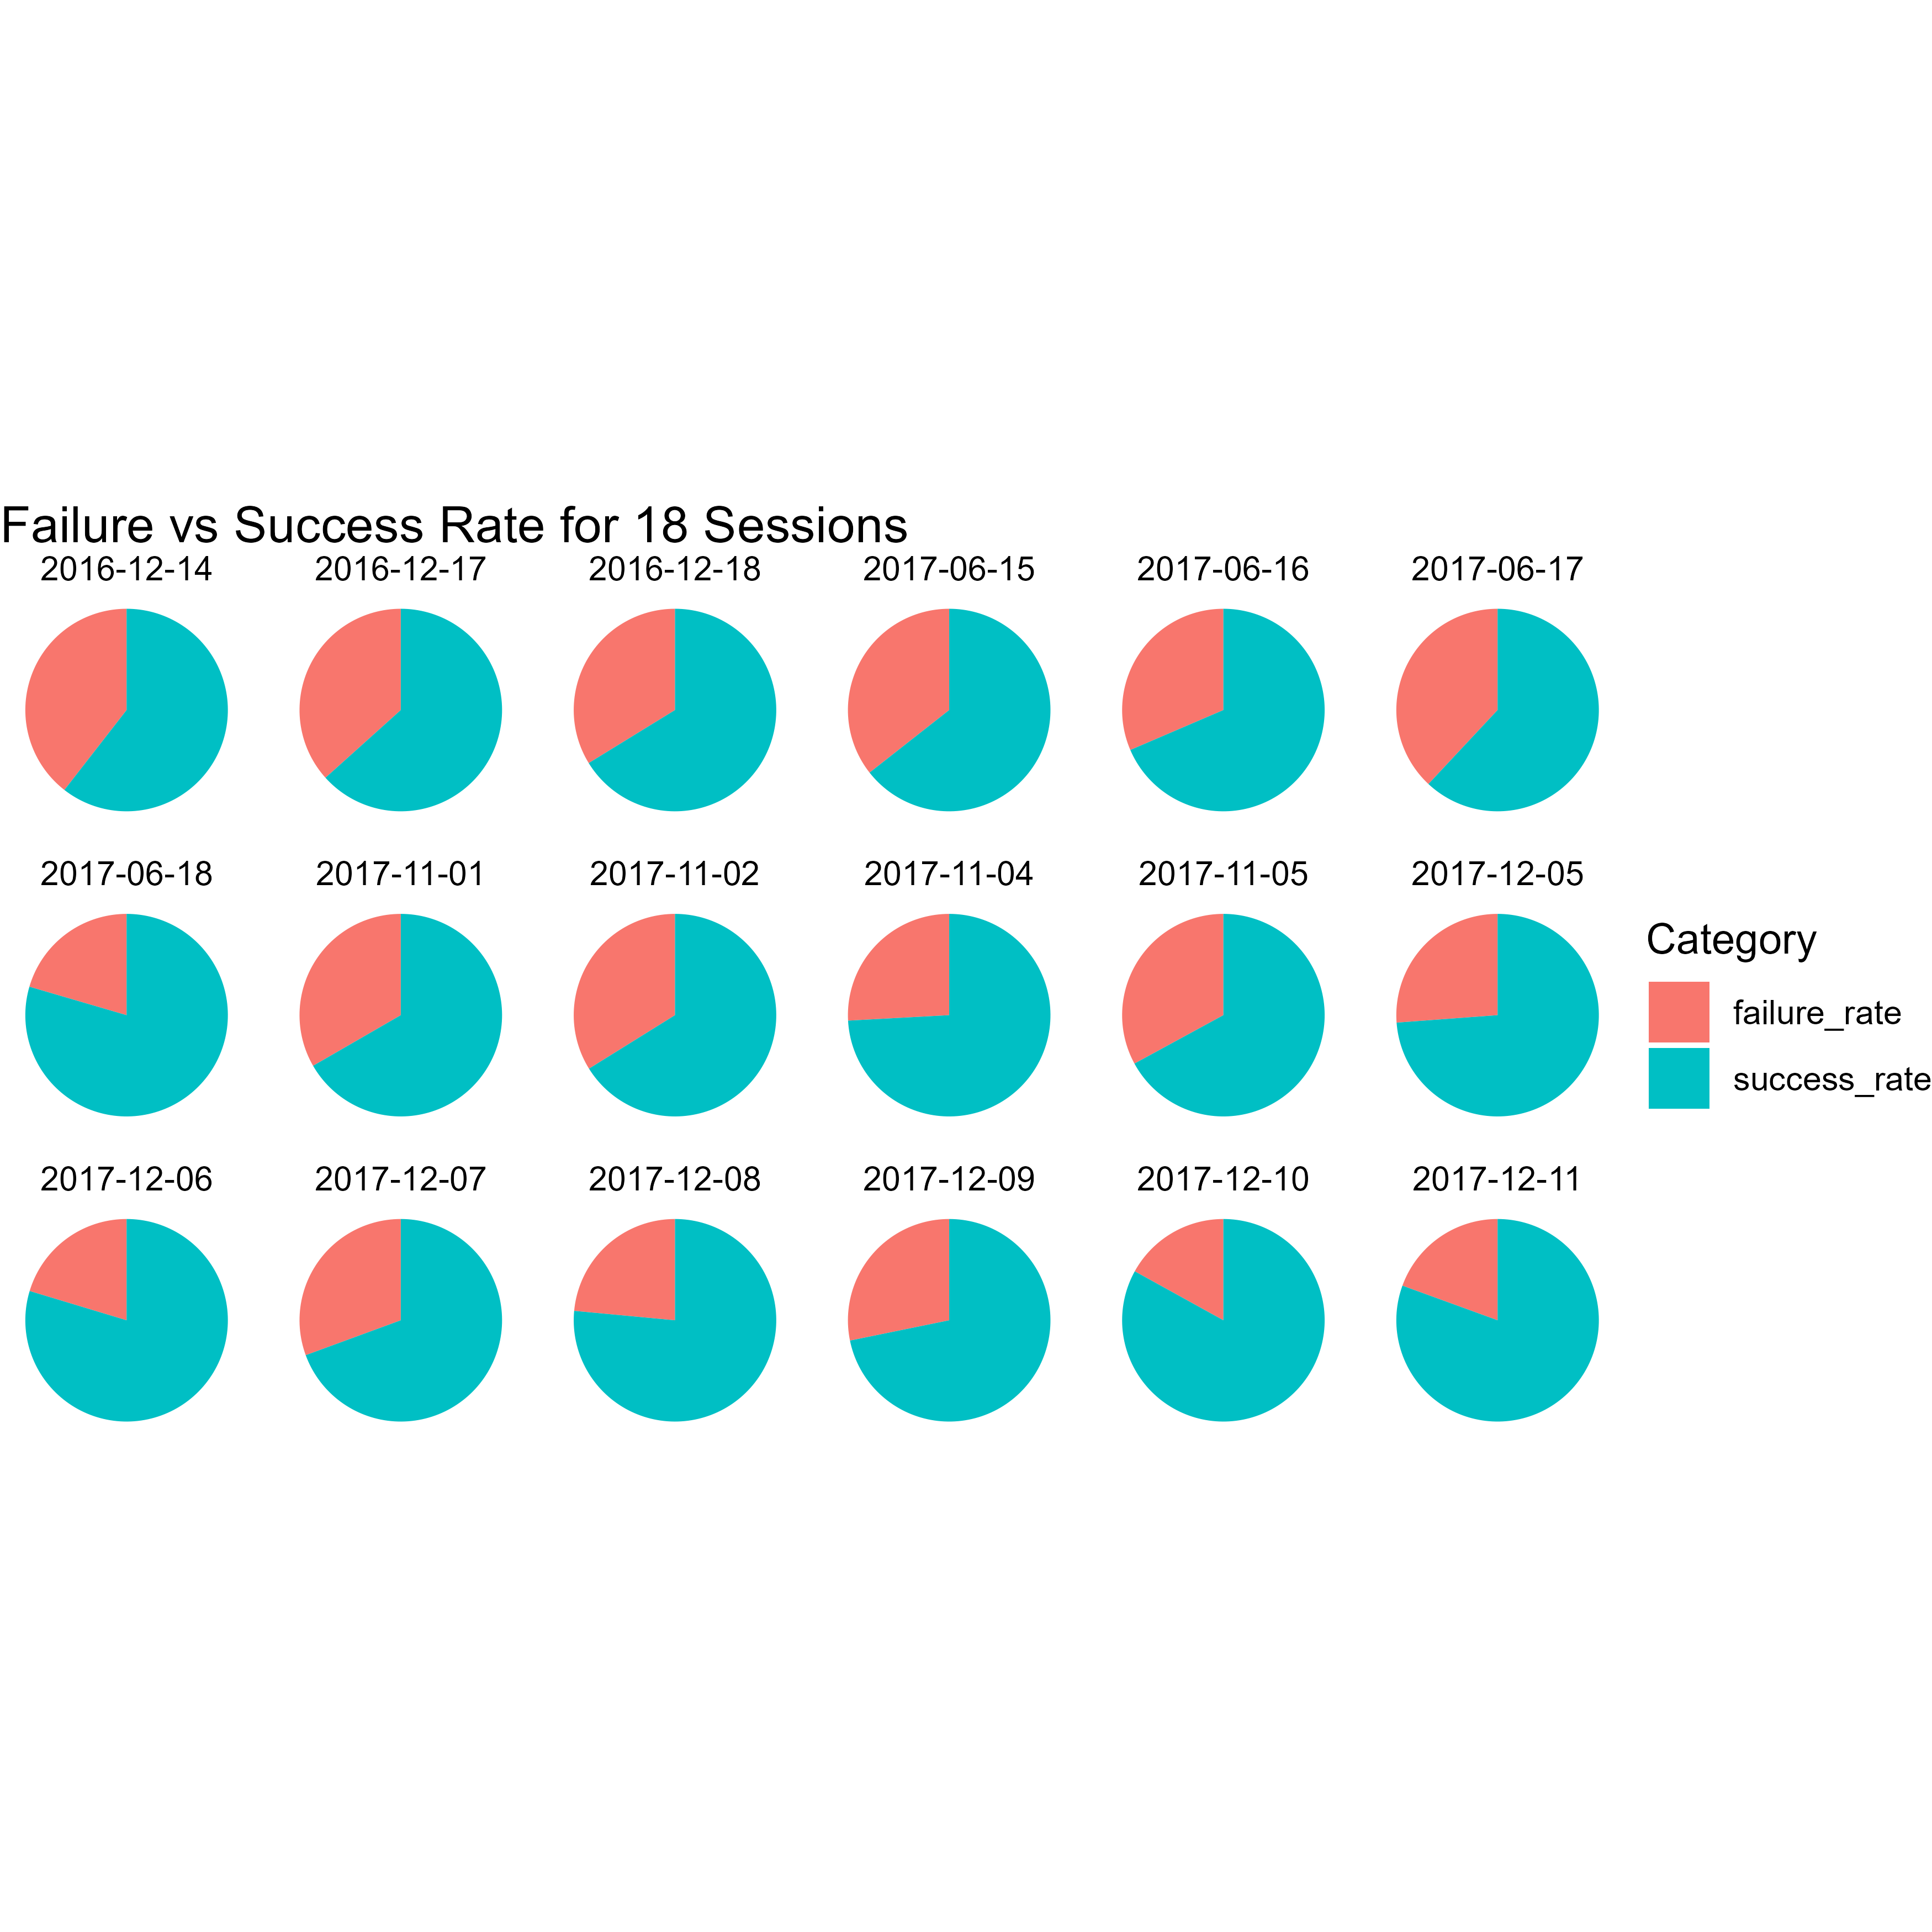
\includegraphics[scale = 0.5]{Pics/006}
		\caption{The Success Rate and the Failure Rate Pie Chart for Every Session}
		\label{fig:006}
	\end{figure}
	\par Moreover, we can explore the successful heat map for all trials and for each mouse, as the heat maps shown below.
	\begin{figure}[htbp]
		\centering
		\begin{minipage}[t]{0.48\textwidth}
			\centering
			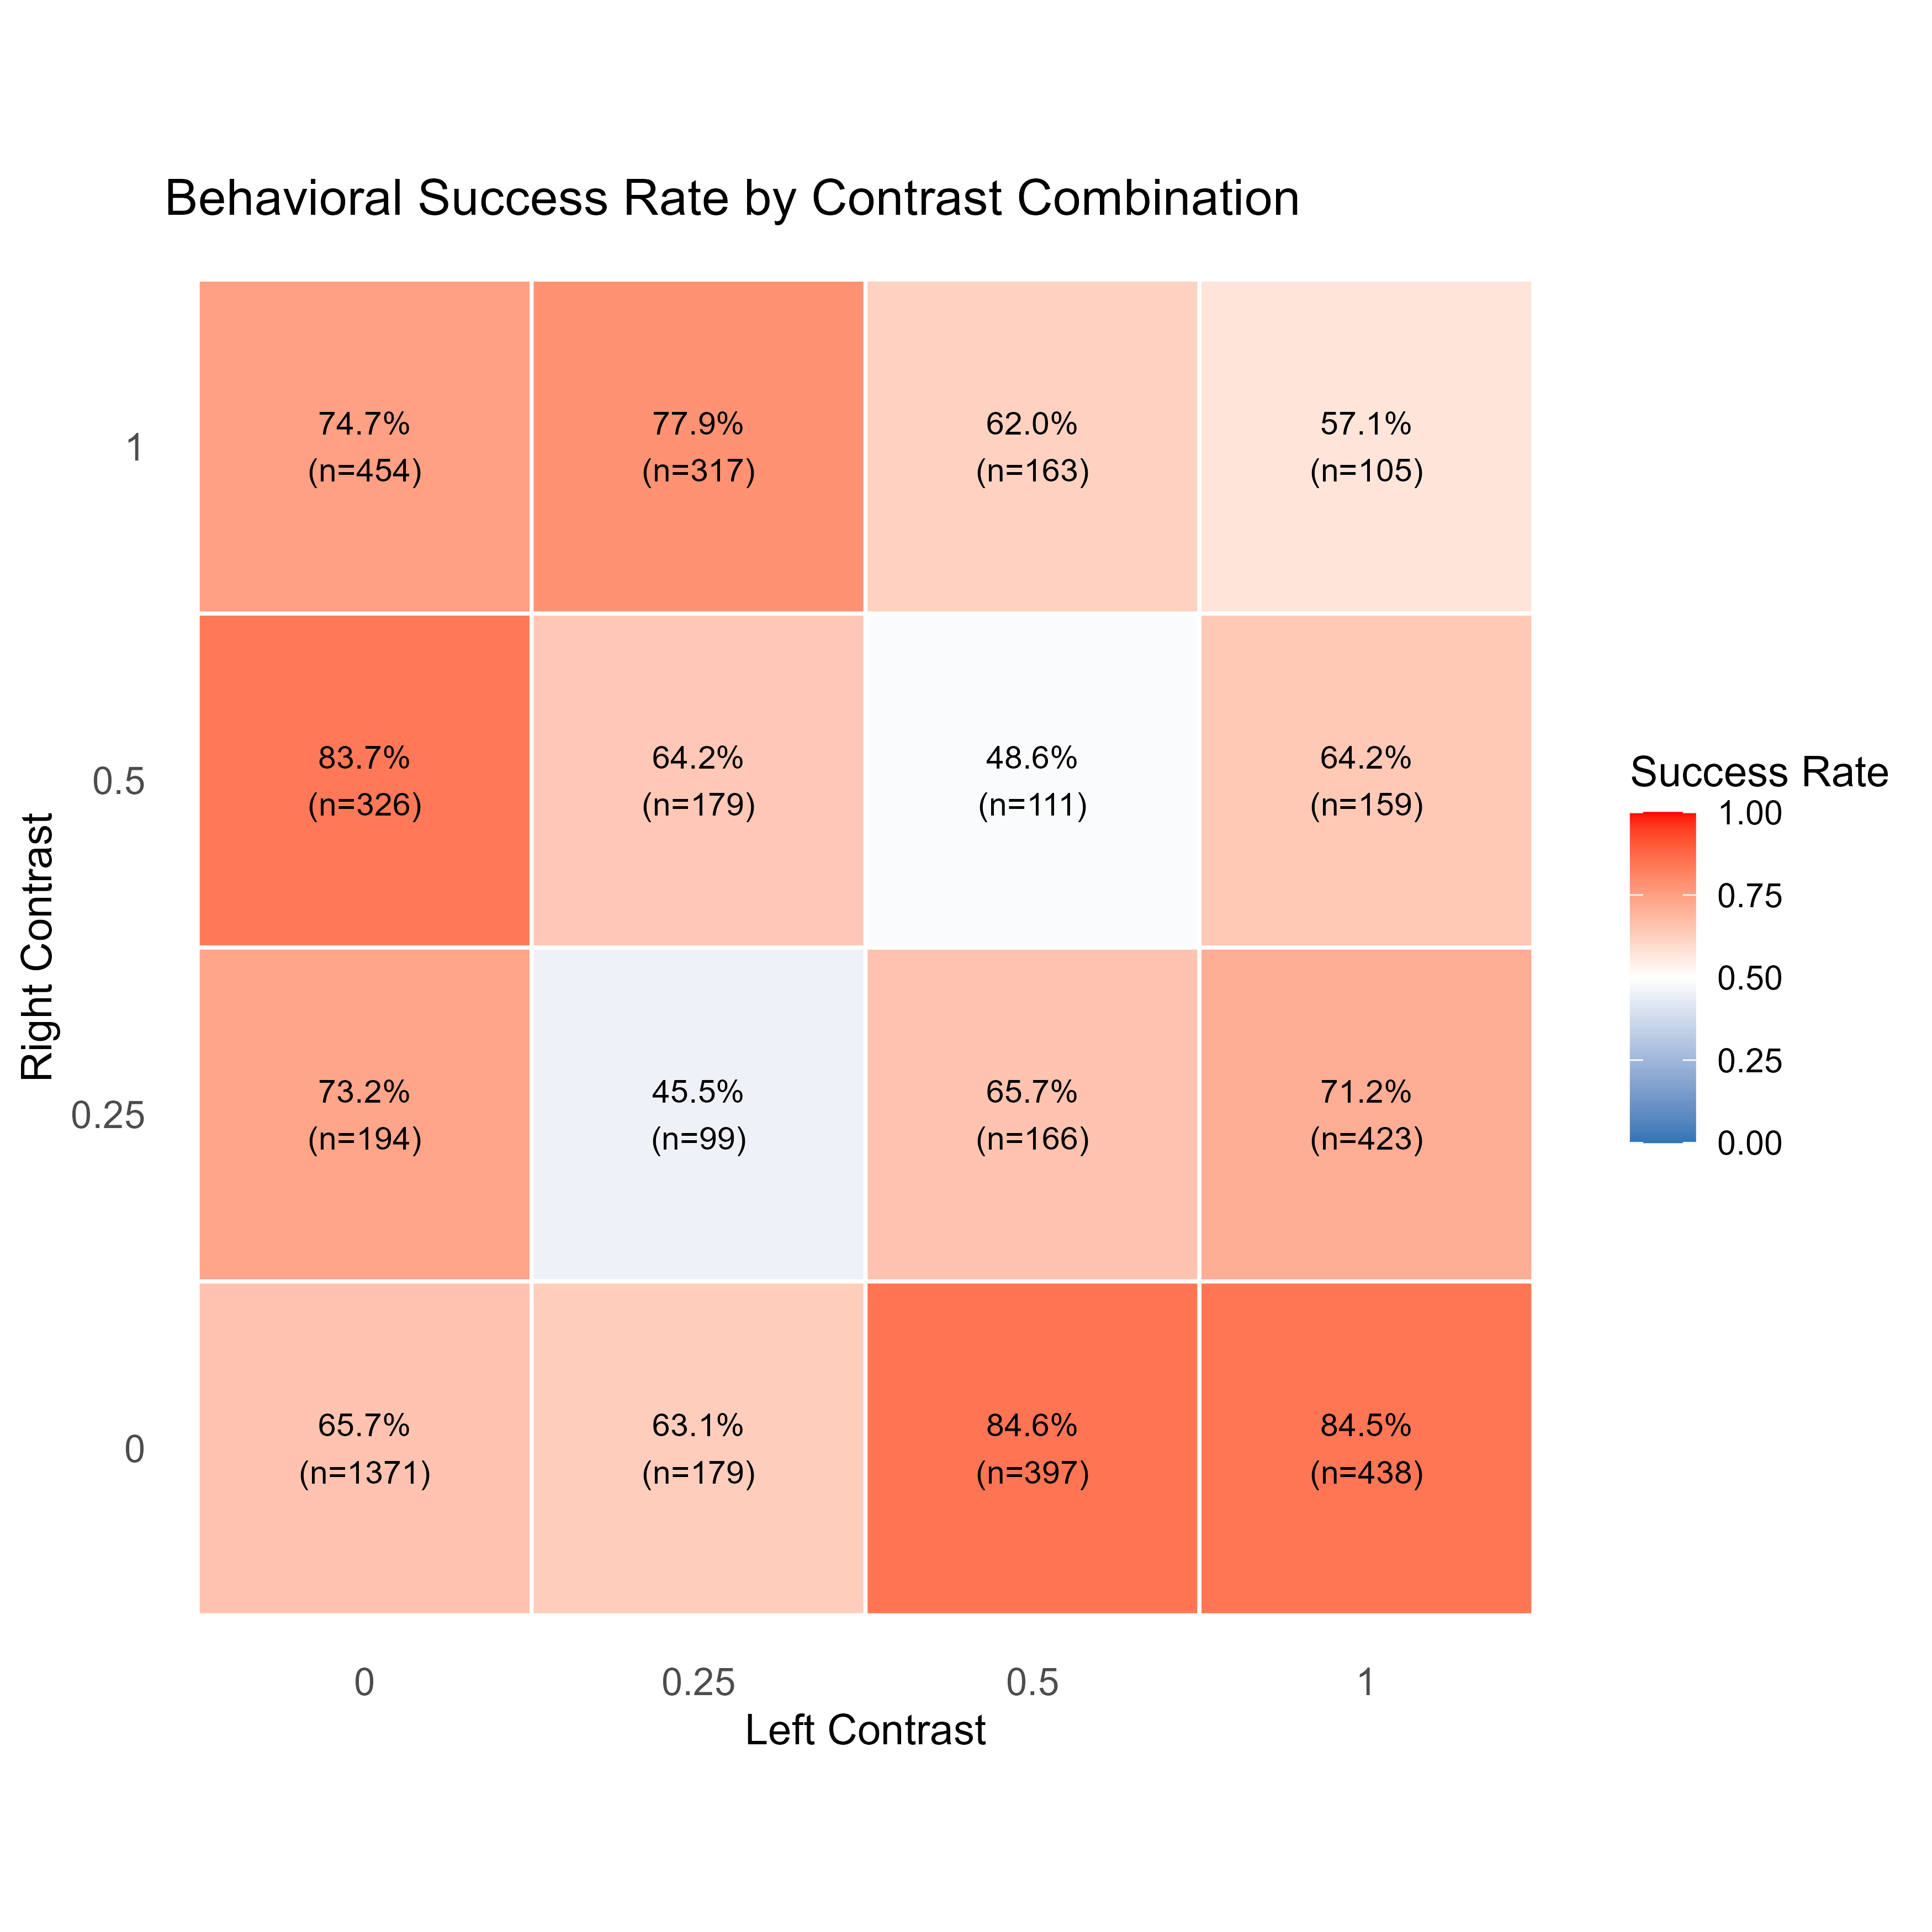
\includegraphics[scale=0.4]{Pics/002}\label{fig:1.3}
			\caption{The Population Heat Map}
		\end{minipage}
		\begin{minipage}[t]{0.48\textwidth}
			\centering
			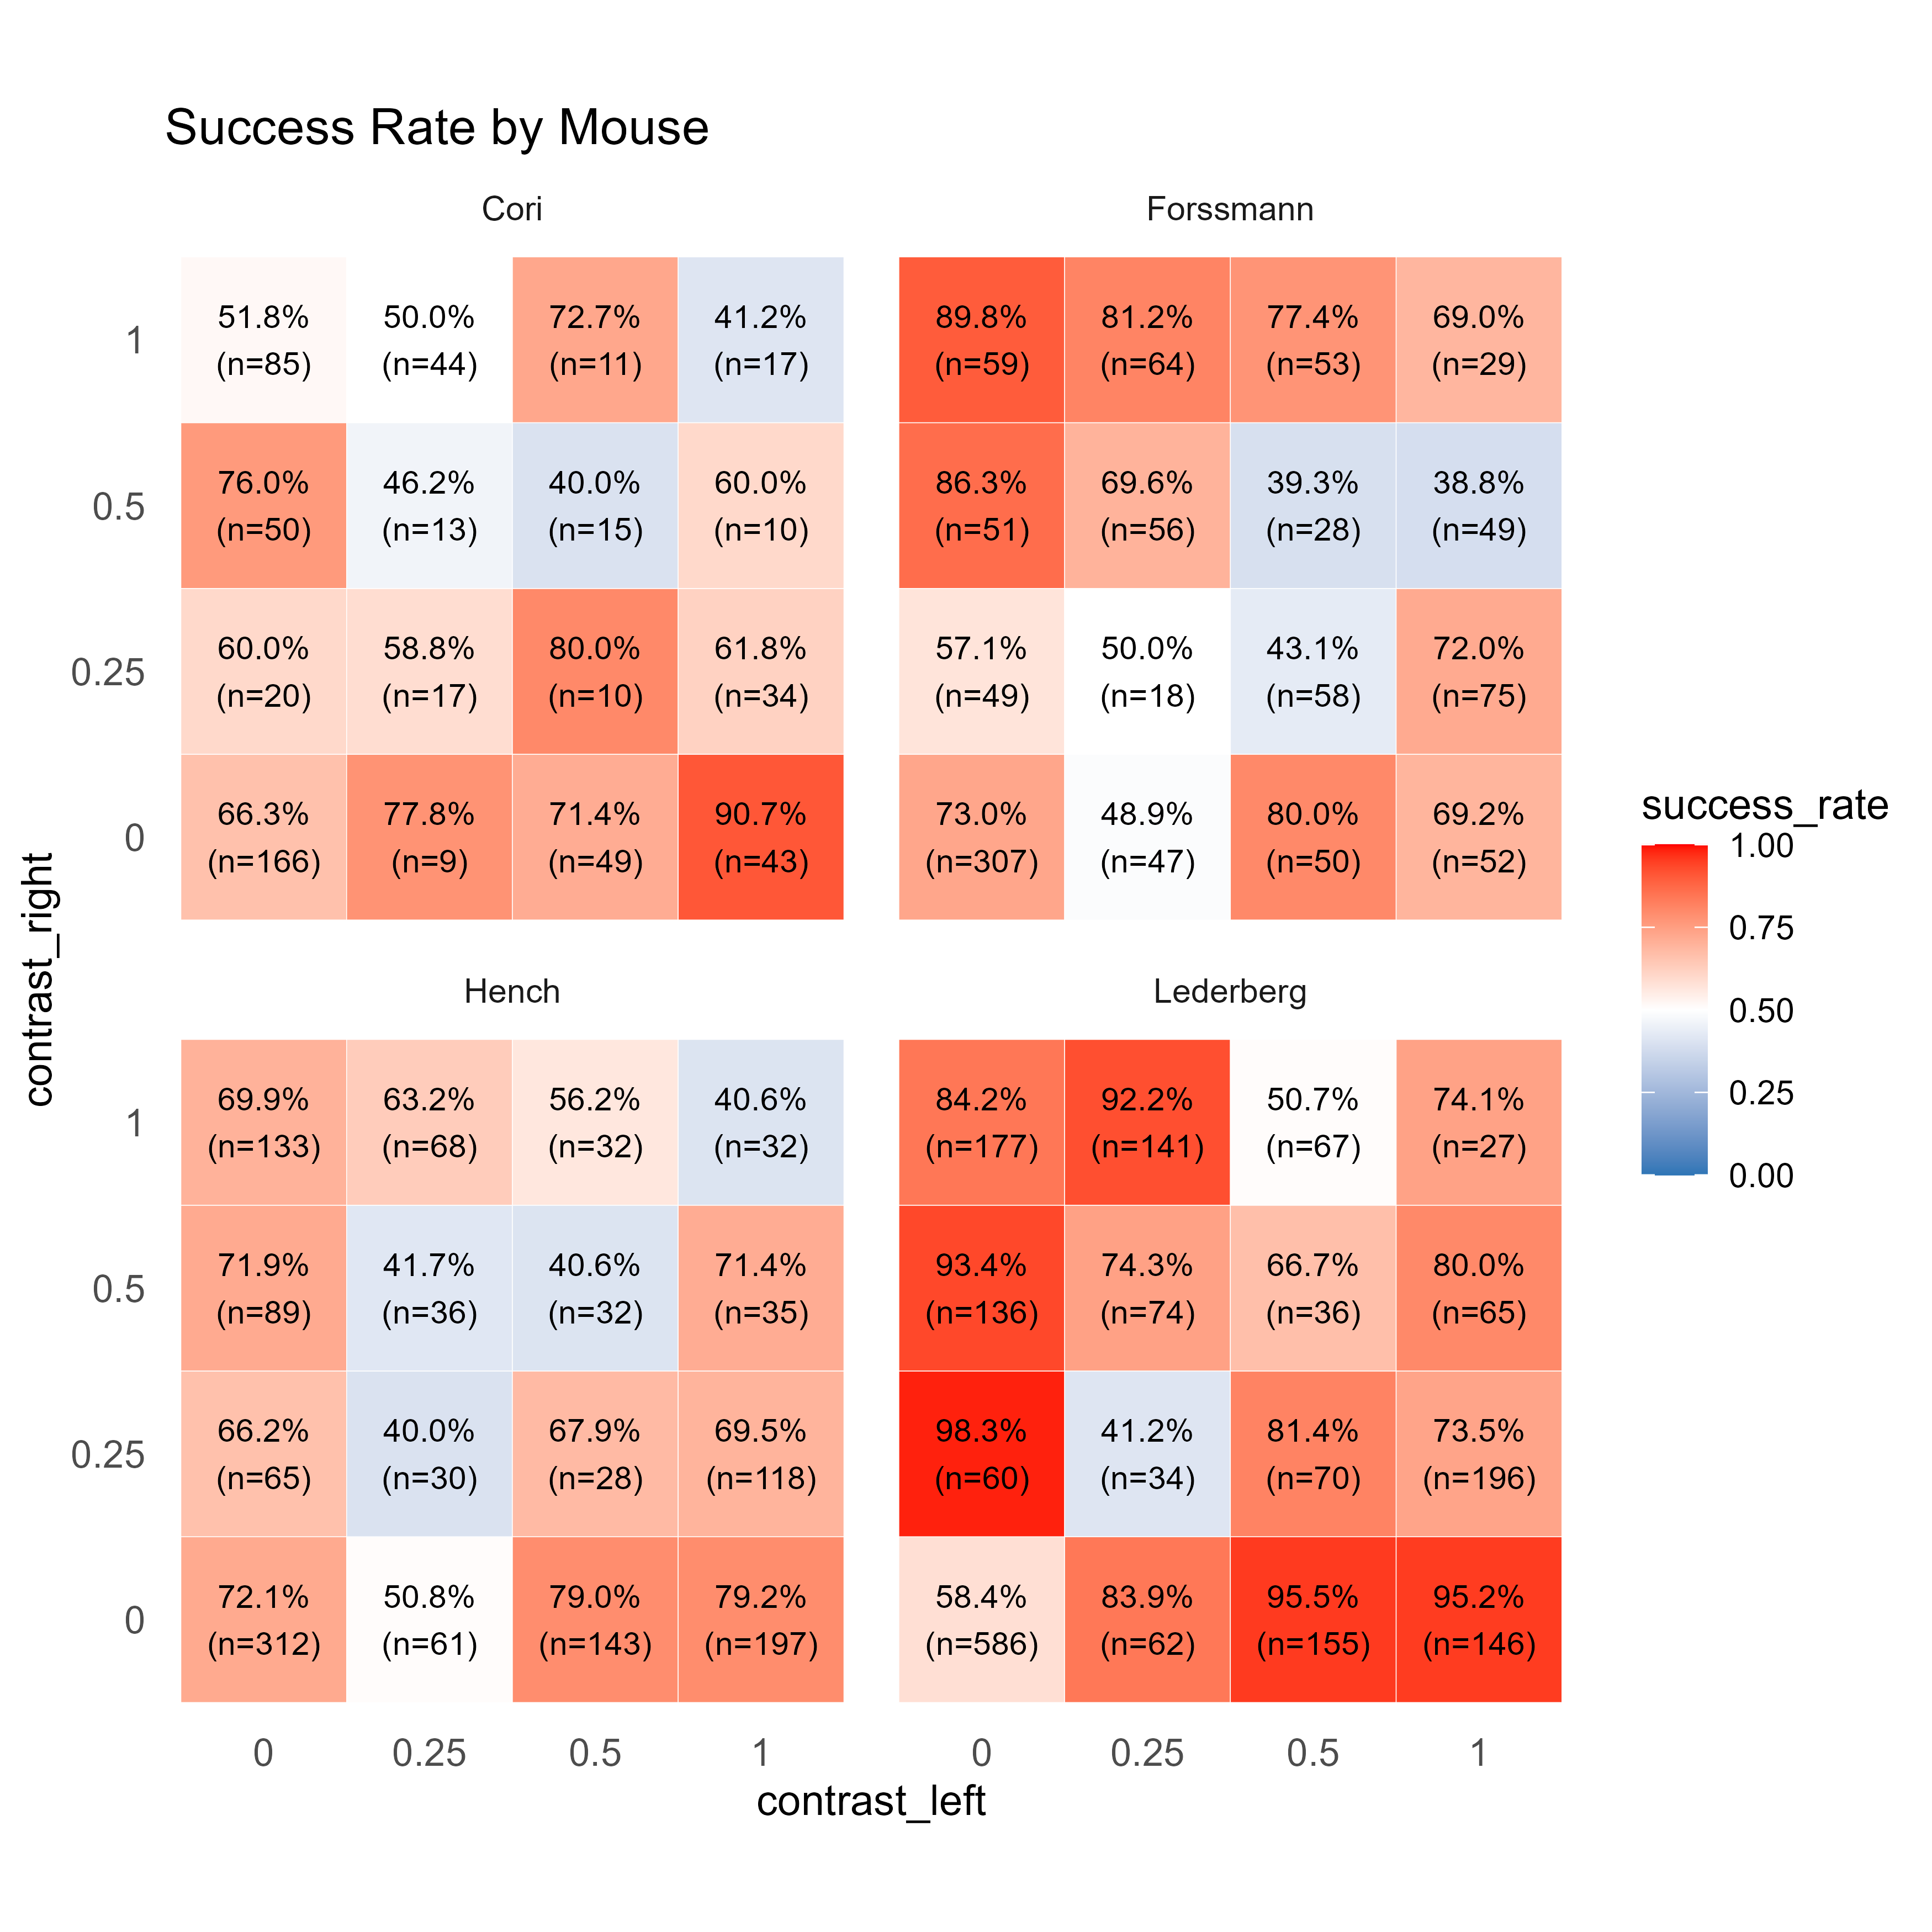
\includegraphics[scale=0.4]{Pics/003}\label{fig:1.4}
			\caption{The Heat Map for Each Mouse}
		\end{minipage}
	\end{figure}
	\par As we can see, for easy cases, the success rate is usually higher than $50\%$, but for more difficult cases, the color of blocks turns to blue and white, which means less or around $50\%.$
\clearpage
	\subsection{The Neural Activities during Each Trial}
	\par Now, with a preliminary understanding of our data, we now dive into the neural activities during each trial, then across trials in the next section. This part of analysis explores the patterns of neural activities each trial. Firstly, we take one special neural and plotted the spike counts of it over time bins, then we plotted the neural population's average activity.
	\subsubsection{Single Neural Activities during Each Trial}
	\par We take the Neuron with id $1$ in the dataset as our observing object. It has $203240$ rows in total, with $6$ columns which has the names: 'session\_id', 'mouse', 'trial\_id', 'neuron\_id', 'time\_bin', 'spike\_count'. And the first $6$ rows are shown in the table below.
	\begin{table}[htbp]
		\begin{tabular}{ccccccc}
			\toprule
			\textbf{session\_id} & \textbf{mouse} & \textbf{brain\_area} & \textbf{trial\_id} & \textbf{neuron\_id} & \textbf{time\_bin} & \textbf{spike\_count} \\
			\midrule
			2016-12-14 & Cori & ACA & 1 & 1 & 1 & 0 \\
			2016-12-14 & Cori & ACA & 1 & 1 & 15 & 0 \\
			2016-12-14 & Cori & ACA & 1 & 1 & 29 & 0 \\
			2016-12-14 & Cori & ACA & 1 & 1 & 3 & 0 \\
			2016-12-14 & Cori & ACA & 1 & 1 & 17 & 0 \\
			2016-12-14 & Cori & ACA & 1 & 1 & 31 & 0 \\
			\bottomrule
		\end{tabular}
		\centering
		\caption{Neural Activity Data}
		\label{tab:neural_activity}
	\end{table}
	\par As we can see, this neuron has the 1st number from the experiment held on 2016-12-14, which is from ACA brain area, meaning Anterior Cingulate Area, and it does not has any spike in time bin 1, 15, 29, 3, 17, 31, i.e. no signal during the six time intervals: 0-0.01s, 0.02-0.03s, 0.14-0.15s, 0.16-0.17s, 0.28-0.29s, 0.30-0.31s in the 1st trial, with a mouse named ``Cori''.
	\par The different brain areas are shown in the graph below from the Ref\cite{ref1} which originally from Ref\cite{ref2}, where the ACA can be easily found.
	\begin{figure}[htbp]
		\centering
		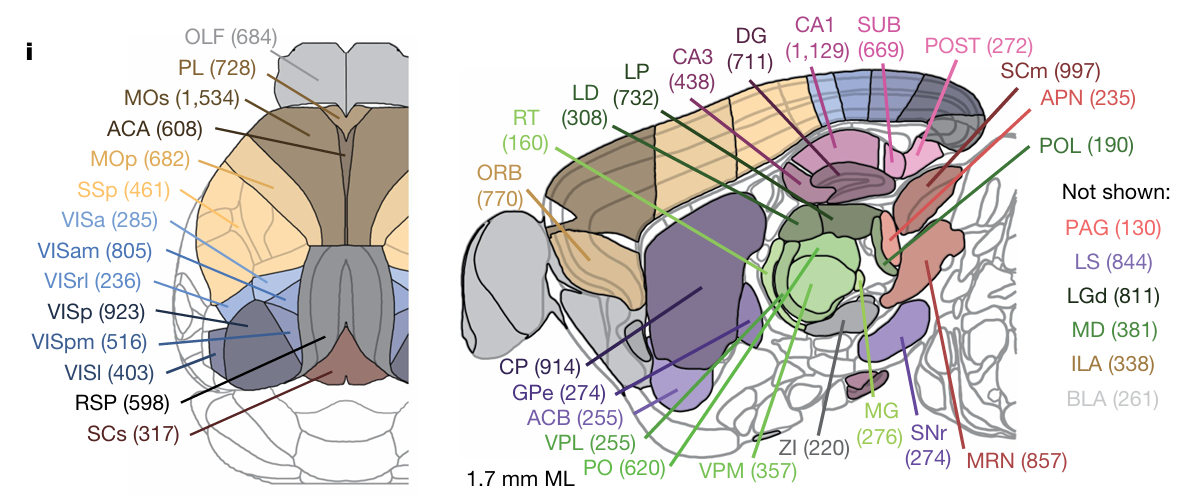
\includegraphics[scale = 0.6]{Pics/007}
		\caption{Different Brain Area for Mouse}
		\label{fig:007}
	\end{figure}
	\clearpage
	Moreover, we should notice that the ``neuron\_id'' is only unique during one session, see the corresponding table below.
	\begin{table}[htbp]
		\begin{tabular}{llr}
			\toprule
			\textbf{session\_id} & \textbf{neuron\_id} & \textbf{brain\_area} \\
			\midrule
			2016-12-14 & 1 & ACA \\
			2016-12-17 & 1 & CA1 \\
			2016-12-18 & 1 & DG \\
			2017-06-15 & 1 & ILA \\
			2017-06-16 & 1 & TT \\
			2017-06-17 & 1 & MB \\
			2017-06-18 & 1 & MOp \\
			2017-11-01 & 1 & LGd \\
			$\vdots$   &1  &$\vdots$\\
			2017-12-09 & 1 & SSs \\
			2017-12-10 & 1 & root \\
			2017-12-11 & 1 & CP \\
			\bottomrule
		\end{tabular}
		\centering
		\caption{Neuron and Brain Area Mapping}
		\label{tab:neuron_brain_area}
	\end{table}
	\par Now, taking the 1st neuron on 2016-12-14, which located at ACA brain area on a mouse named ``Cori'' as our example. 
	\begin{figure}[htbp]
		\centering
		\begin{minipage}[t]{0.48\textwidth}
			\centering
			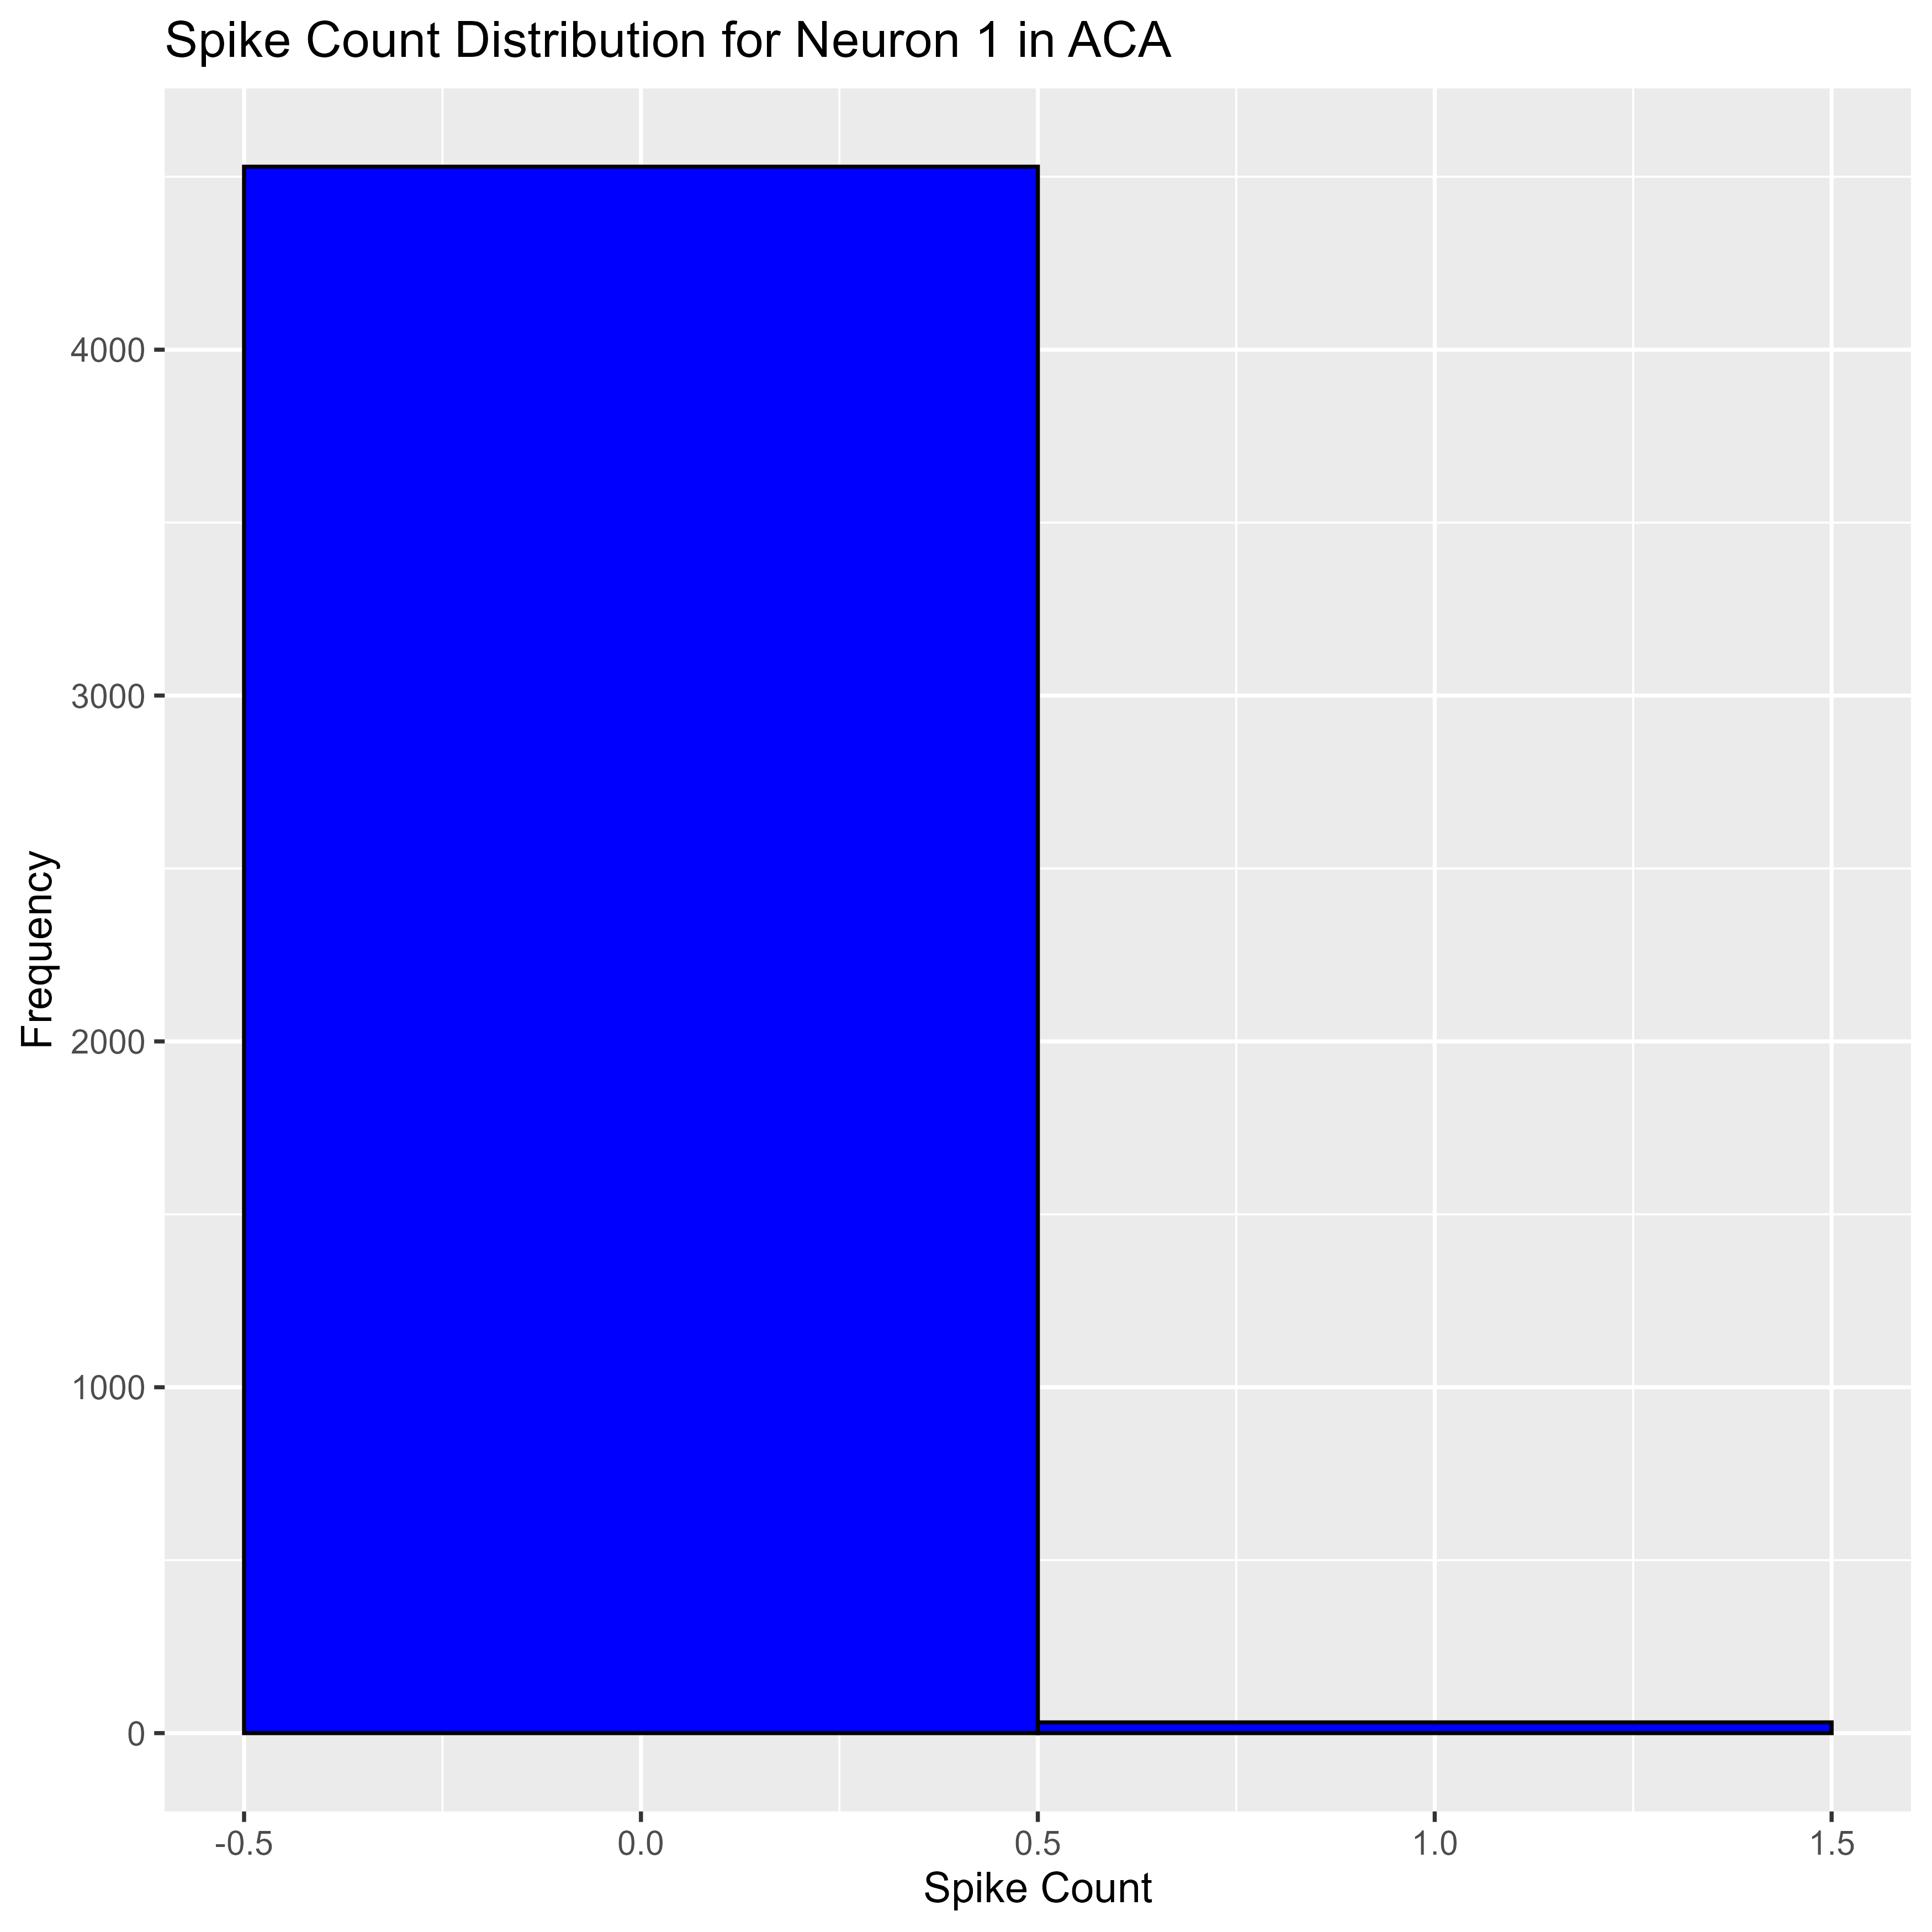
\includegraphics[scale=0.3]{Pics/008}\label{fig:1.8}
			\caption{The Frequency of Spike Counts}
		\end{minipage}
		\begin{minipage}[t]{0.48\textwidth}
			\centering
			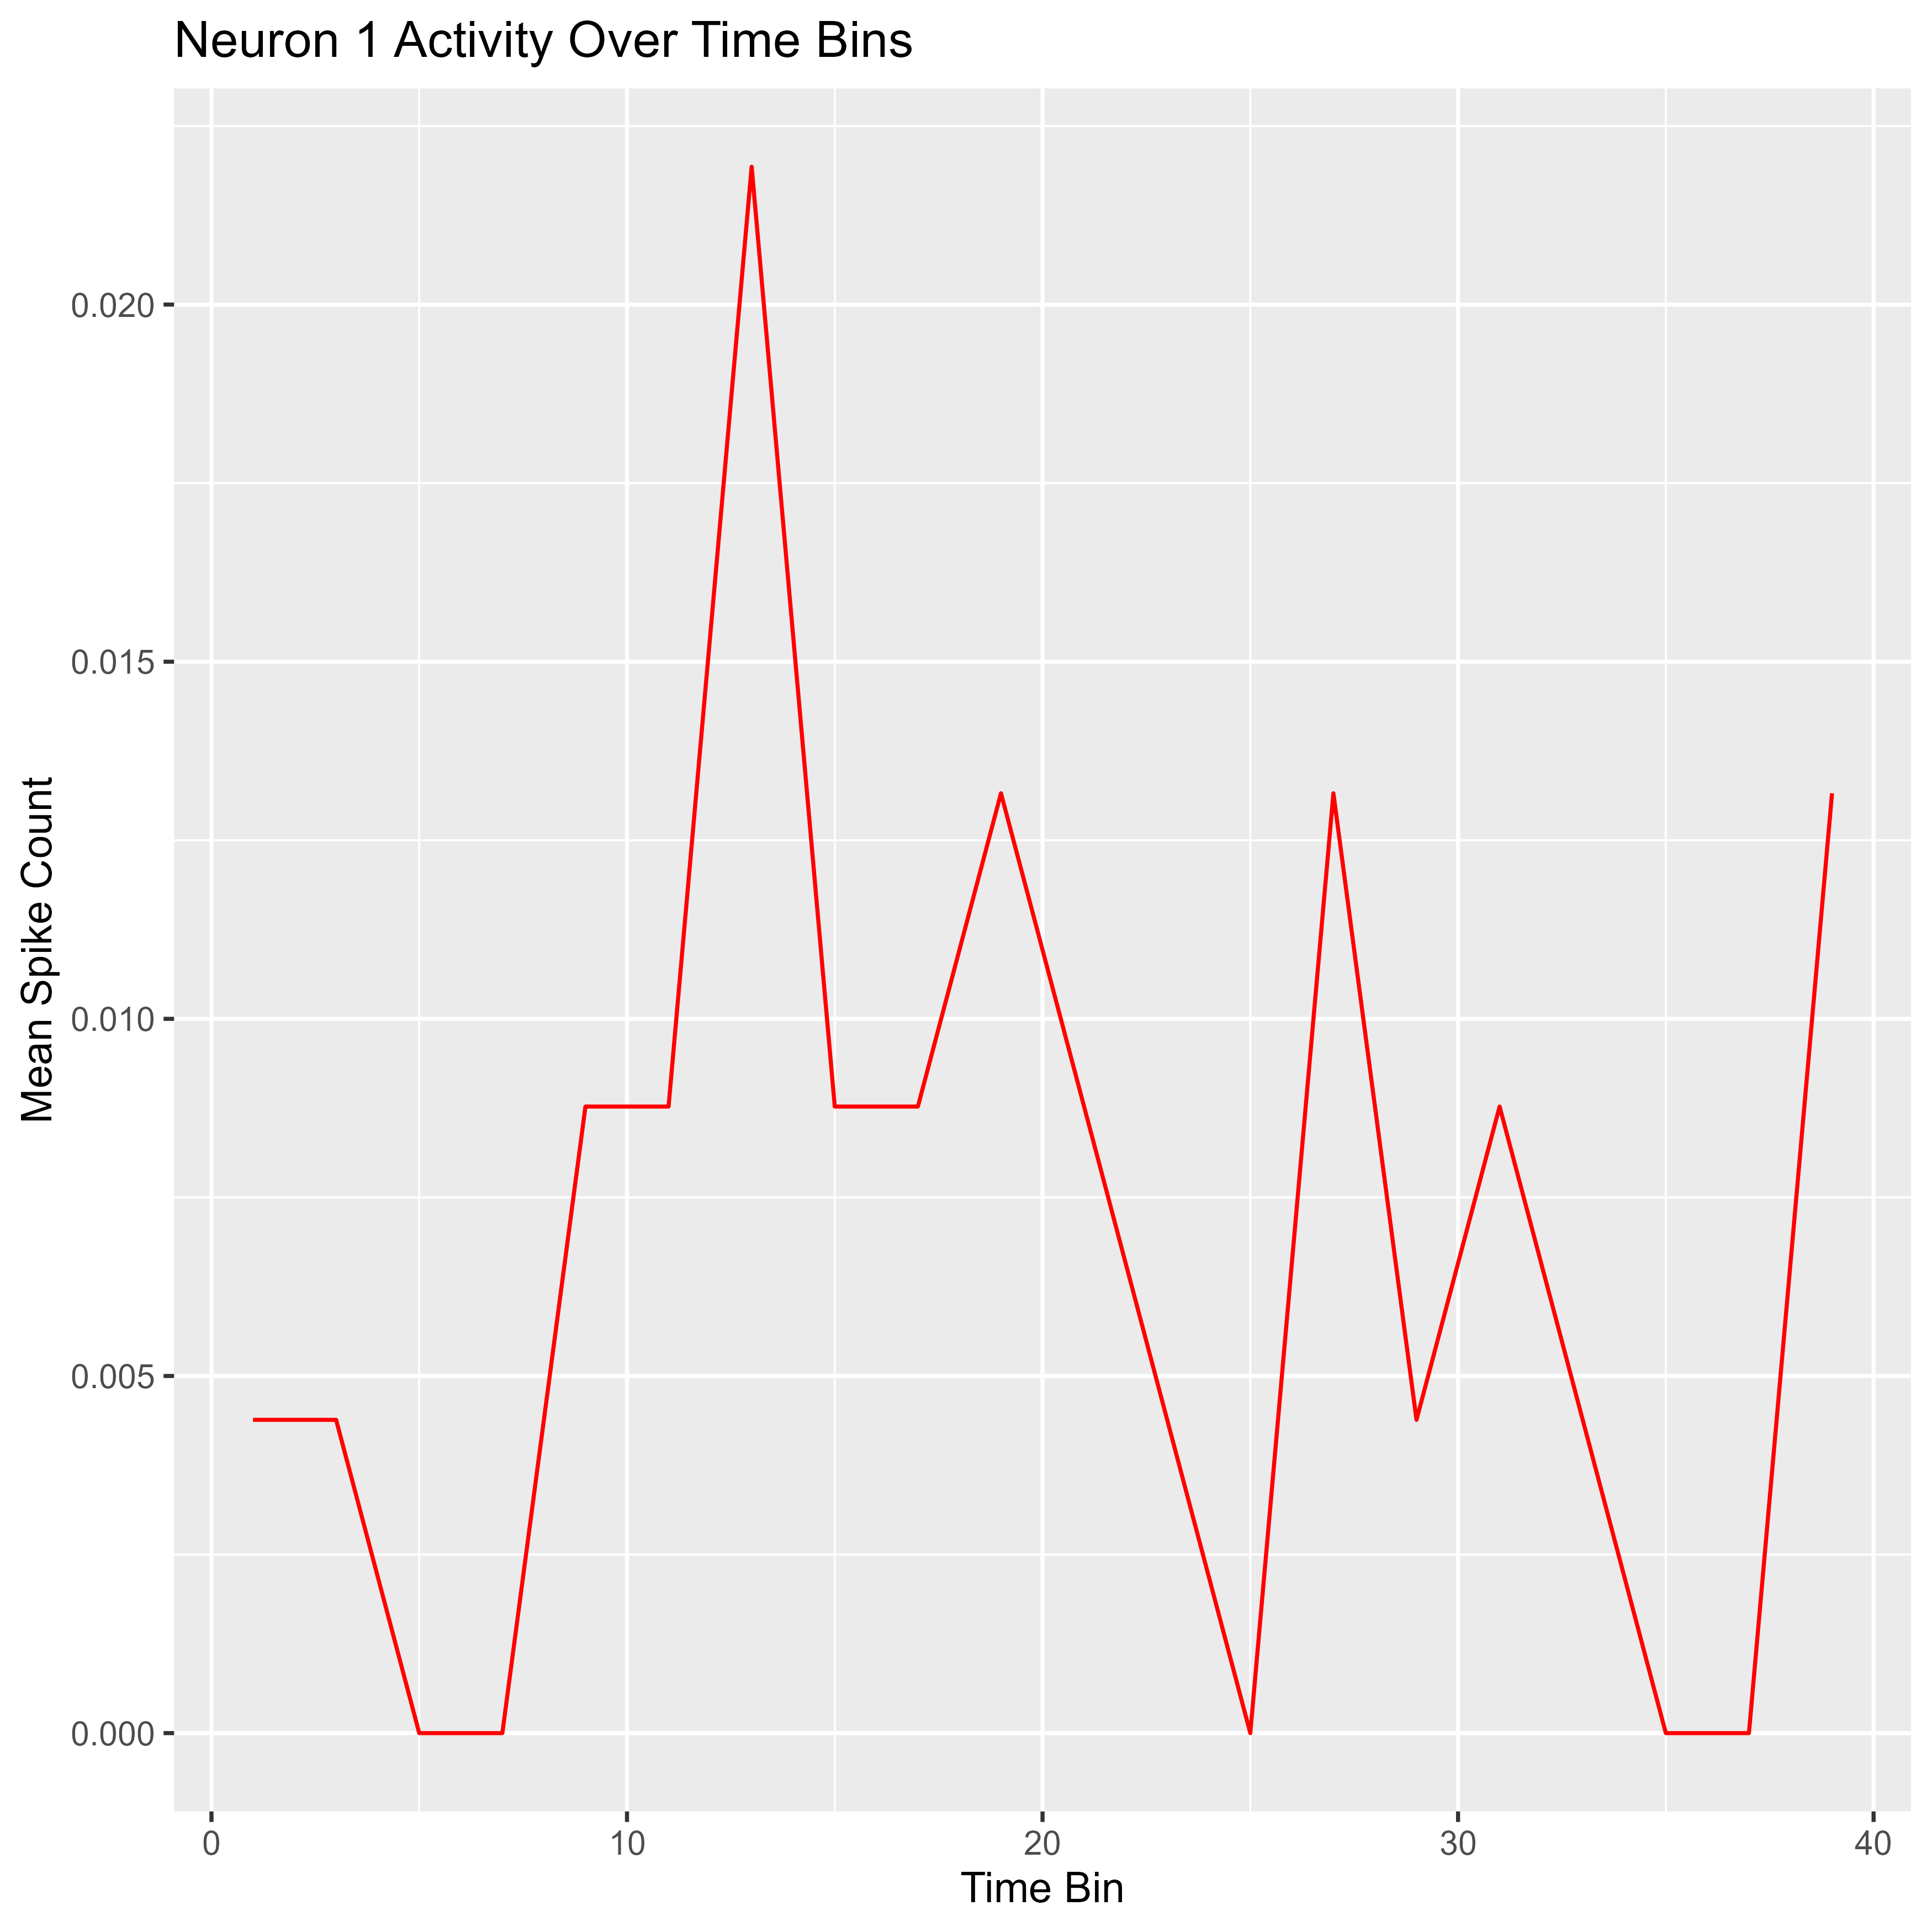
\includegraphics[scale=0.3]{Pics/009}\label{fig:1.9}
			\caption{The Mean Spike Counts v.s. Time Bins}
		\end{minipage}
	\end{figure}
	\par The two graphs above are the histogram of spike counts and the mean spike counts v.s. time bins from 1 to 40. As we can see, this specific neuron is hard to get activated with a frequency less than $0.03$, and usually it is activated around $10-15$ bins, corresponding to $0.1s-0.15s$ in each trial.
	\clearpage
	\subsection{The Neural Activity across Trials}
	\par We examined the neural activity patterns of a single neuron (Neuron 1) over $40$ time bins during a visual discrimination task, as shown below.
	\begin{figure}[htbp]
		\centering
		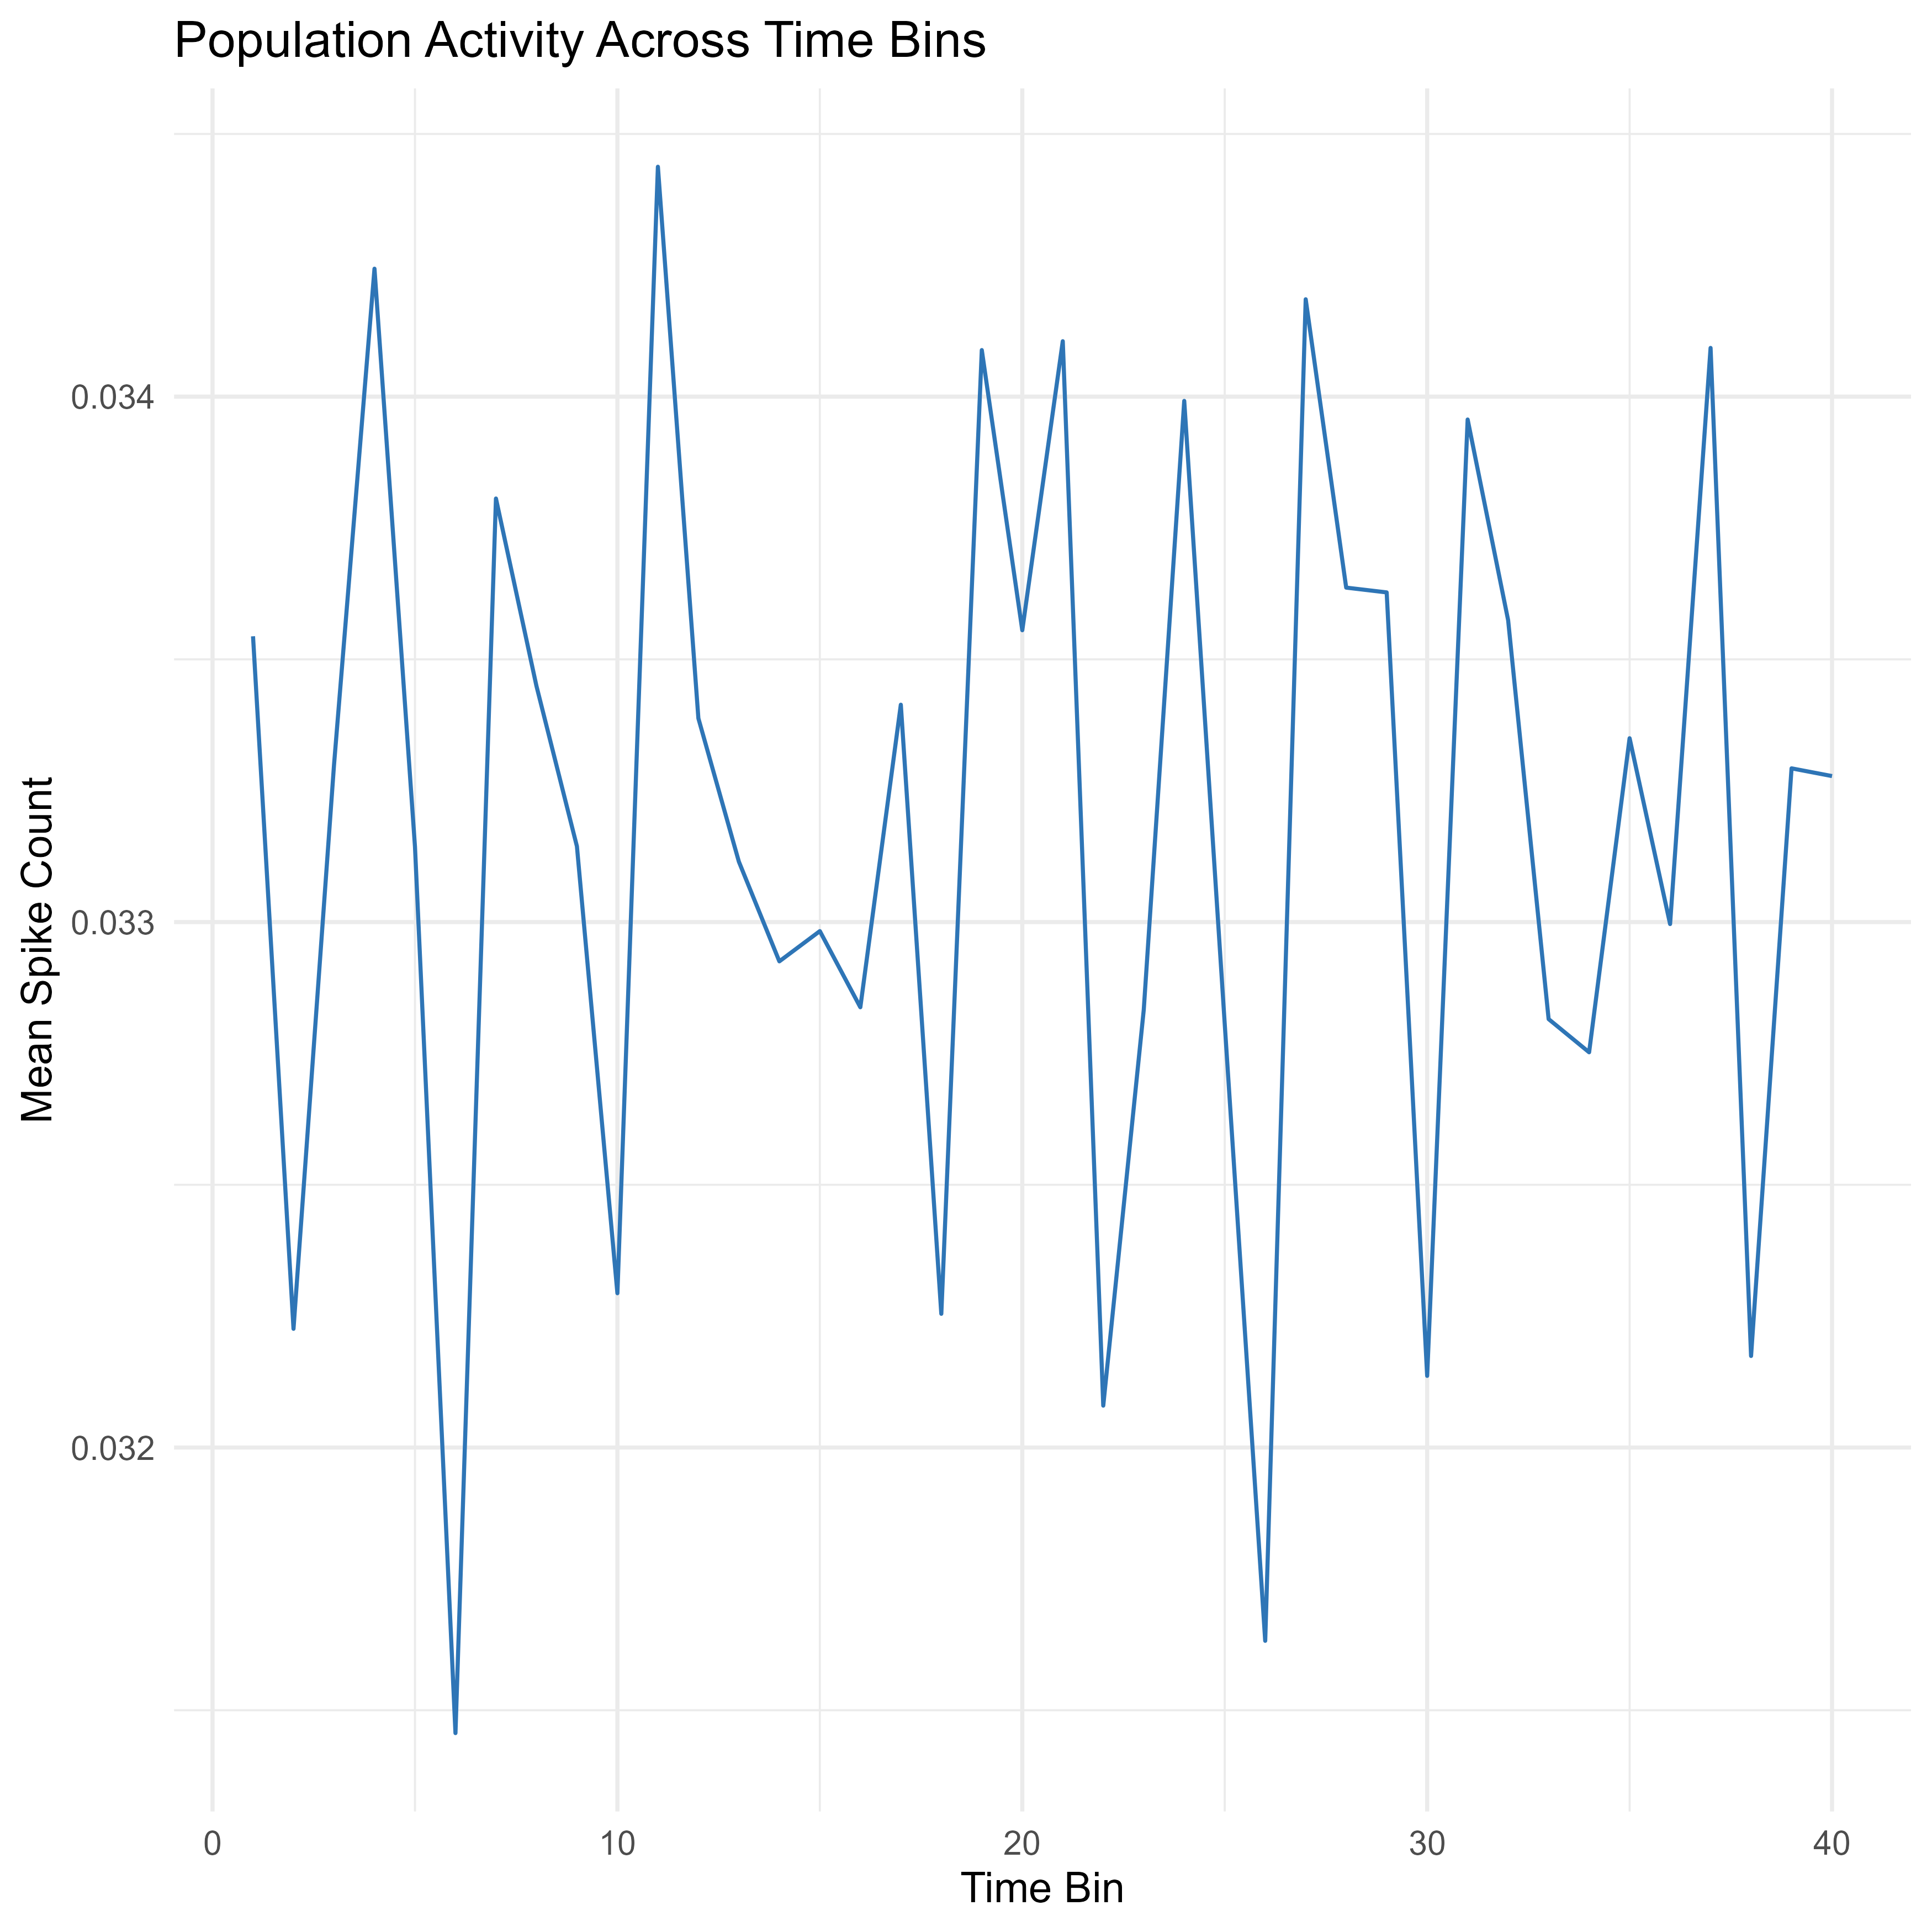
\includegraphics[scale = 0.3]{Pics/010}
		\label{fig:010}
	\end{figure}
	\par Firstly, as shown in the plot, the activity was recorded as spike trains, which were binned into $40$ time intervals (time bins for $0-0.4$s) to quantify the number of spikes in each interval. The mean spike count for each time bin was calculated across trials to generate the activity profile of the neuron over time.
	\par The activity plot for Neuron 1 shows significant \textbf{fluctuations} across the 40 time bins. The neuron exhibits periods of high activity with peak mean spike counts reaching approximately 0.02 spikes/bin, interspersed with periods of low or no activity. Notable peaks occur around time bins 12, 22, 32, and 40, may suggesting potential responses to specific events or stimuli in the task timeline. The neuron's activity demonstrates a non-stationary pattern, indicating dynamic responses that vary over the course of the trial.
	\par Also, we plotted the mean spike counts in different trials, colored with red and blue to represent the outcomes. (red for success and blue for failure)
	\begin{figure}[htbp]
		\centering
		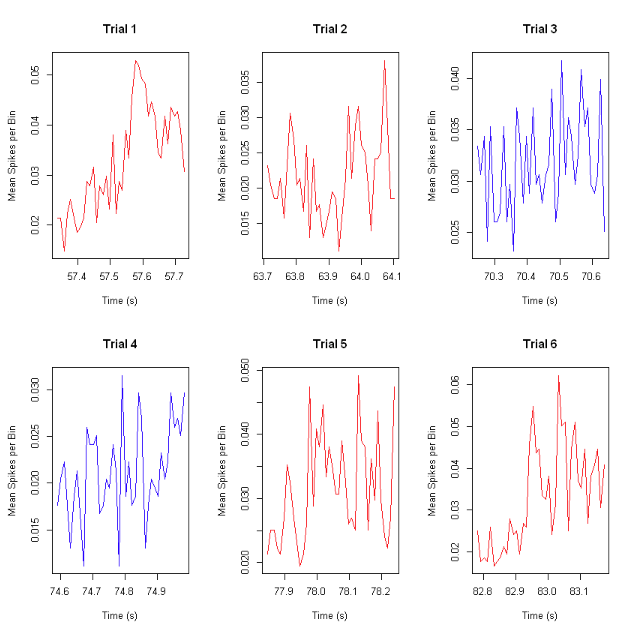
\includegraphics[scale = 0.4]{Pics/021}
		\caption{Mean Spike Counts in Different Trials}
		\label{fig:021}
	\end{figure}
	\clearpage
	\subsection{The Total Spike Counts Across Trials}
	\begin{figure}[htbp]
		\centering
		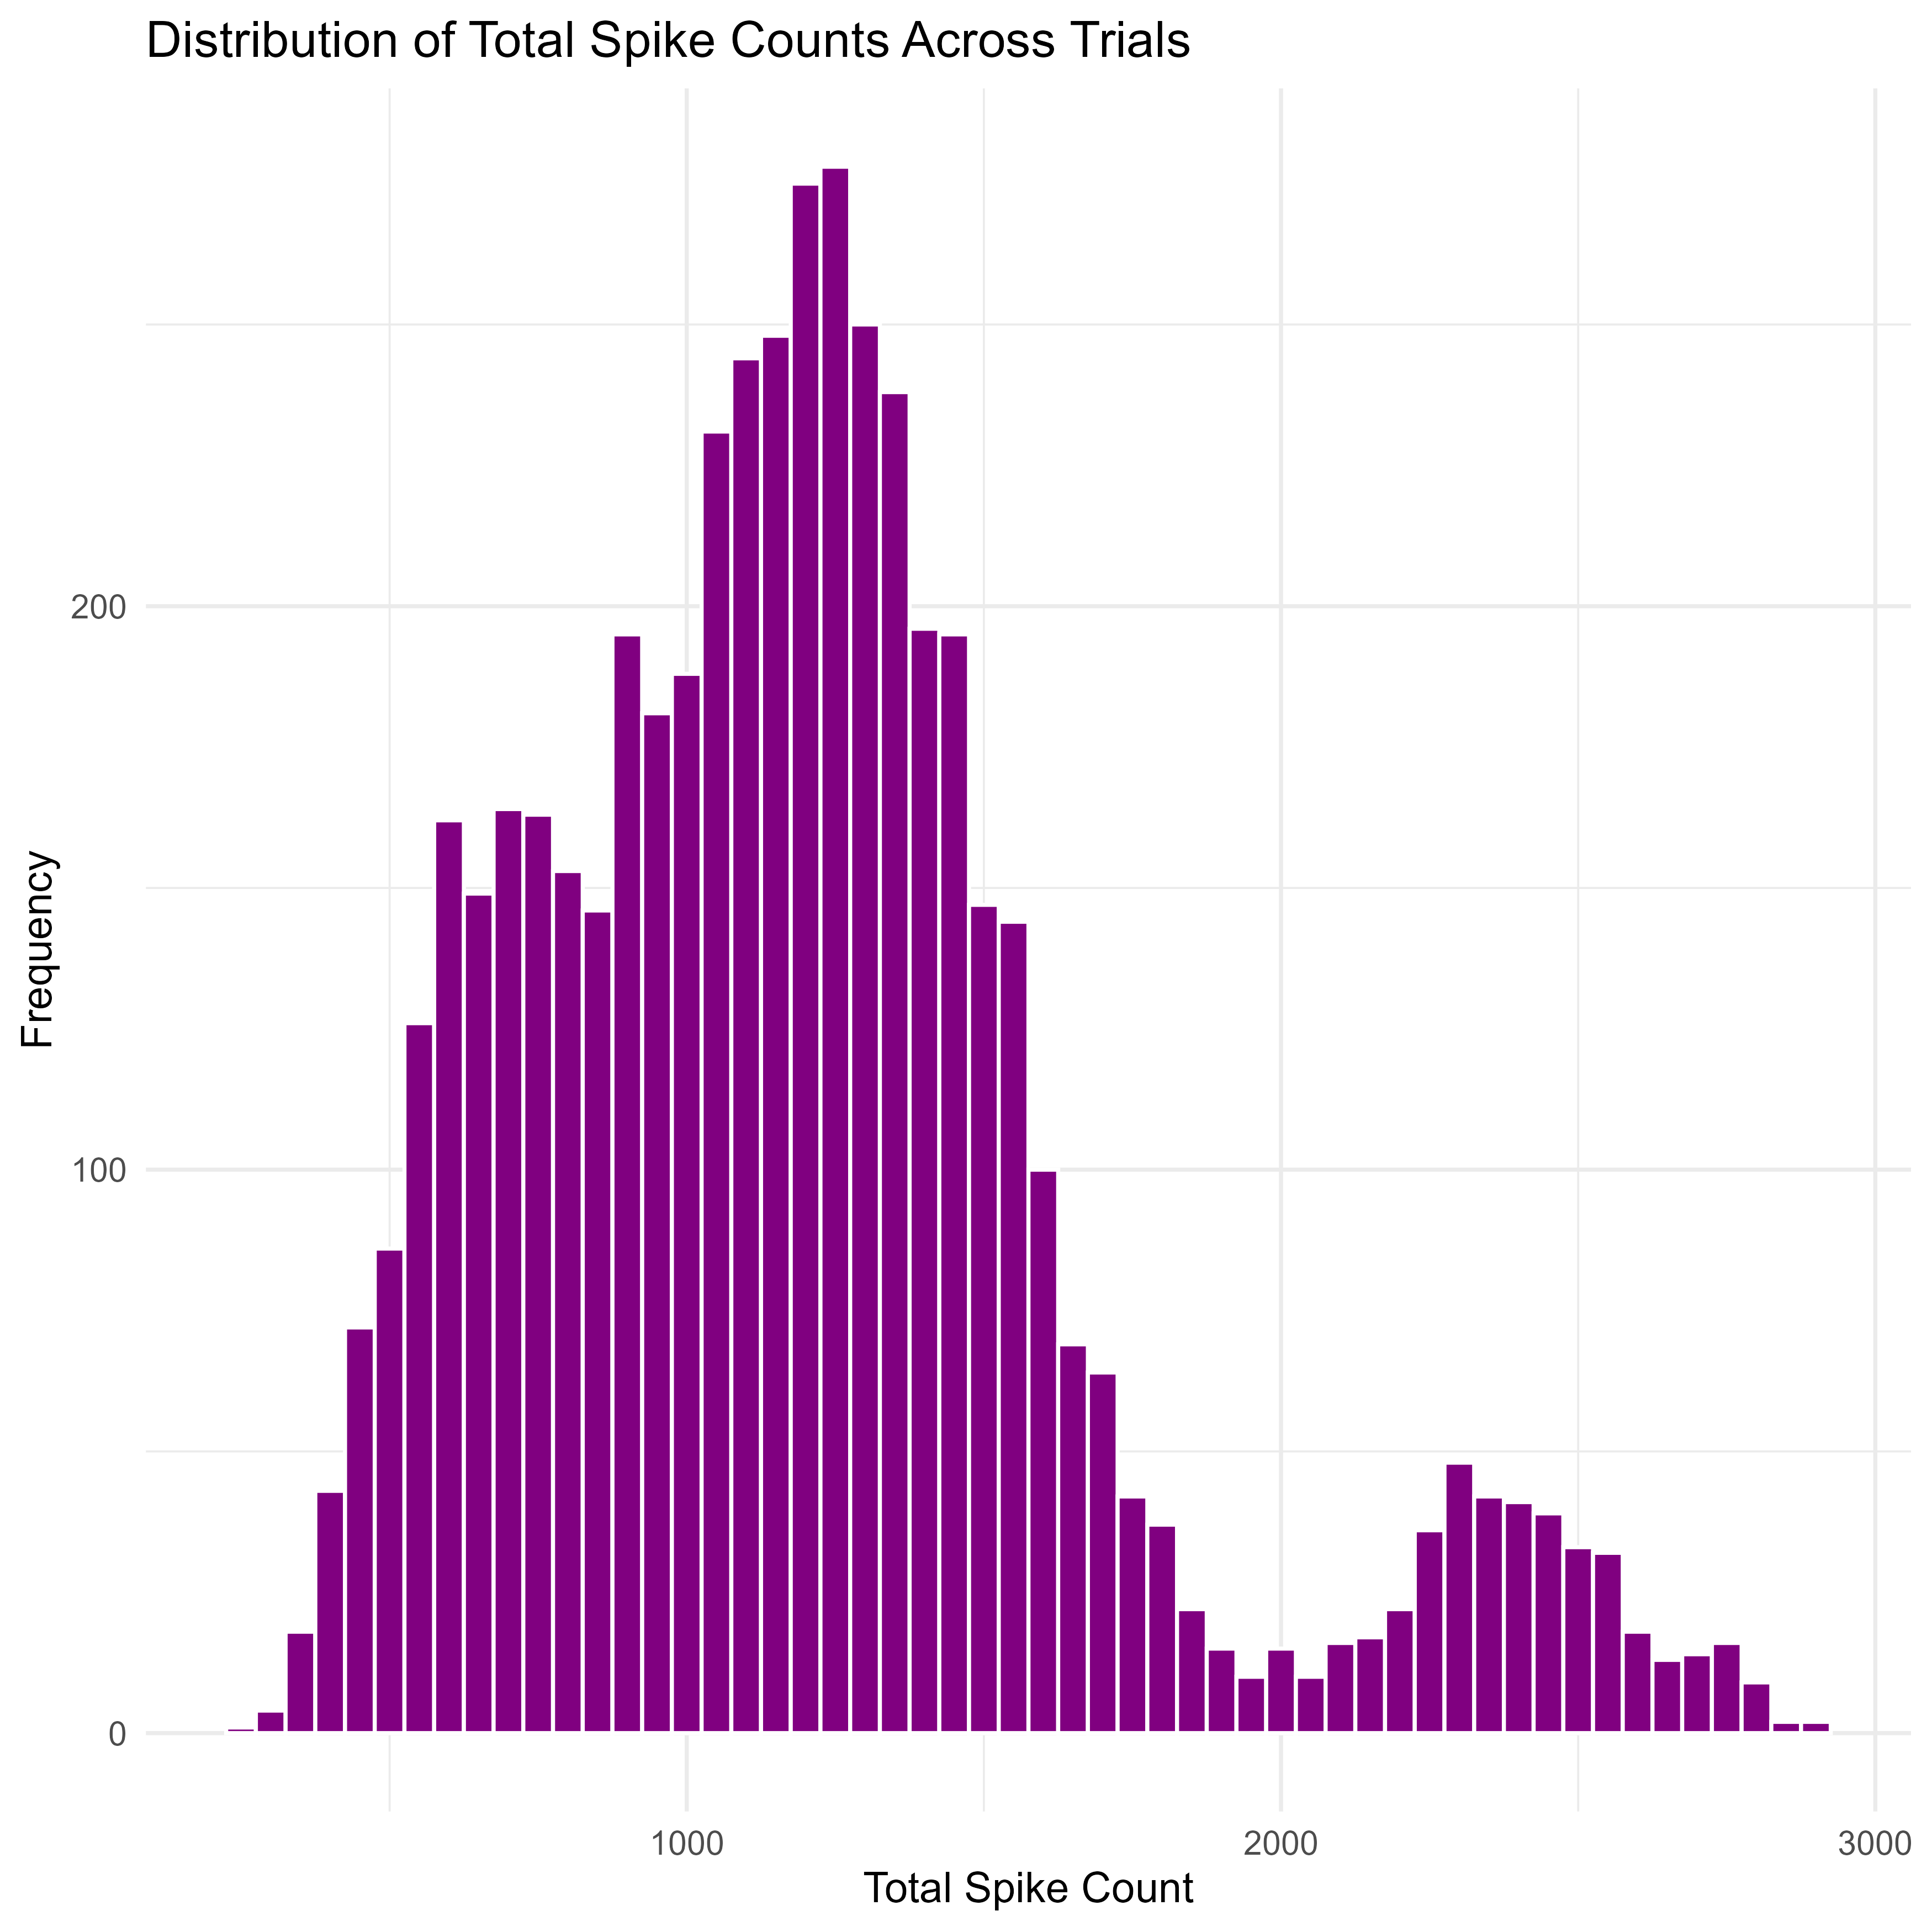
\includegraphics[scale = 0.4]{Pics/011}
		\label{fig:011}
	\end{figure}
	\par The histogram above depicts the distribution of total spike counts across trials for a neuron. The data shows a right-skewed distribution, with a concentration of trials having lower spike counts and a long tail extending towards higher spike counts. This suggests that while most trials result in relatively few spikes, there are occasional trials with significantly higher spike activity. 
	\par The distribution's asymmetry indicates variability in neural response across trials, potentially reflecting different stimuli conditions, behavioral outcomes, or natural variability in neural firing. The spread of the data points around the central tendency provides insight into the reliability and consistency of the neuron's firing pattern during the experimental tasks.
	\clearpage
	\subsection{The Homogeneity and Heterogeneity across Sessions and Mice}
	Now, let's dive into the study for the homogeneity and heterogeneity across sessions and mice. 
	\par We firstly studied the participate situation for each mouse, as the table shows, Cori engaged $3$ sessions, Forssmann engaged $4$ sessions and so on.
	\begin{table}[htbp]
		\centering
		\begin{tabular}{lc}
			\toprule
			\textbf{Mouse Name} & \textbf{Number of Sessions} \\
			\midrule
			Cori                & 3 \\
			Forssmann           & 4 \\
			Hench               & 4 \\
			Lederberg           & 7 \\
			\bottomrule
		\end{tabular}
	\end{table}
	\par Moreover, for each session, we found that the number of neurons is unchanged for every trial in the specific session. With the above information, we can now study the homogeneity and heterogeneity across sessions and mice.
	\subsubsection{Box Plots}
	\par Firstly, we drawn the box plot for $4$ mice and the number of neurons and the success rate in each session to visualize the homogeneity across mice.
		\begin{figure}[htbp]
		\centering
		\begin{minipage}[t]{0.48\textwidth}
			\centering
			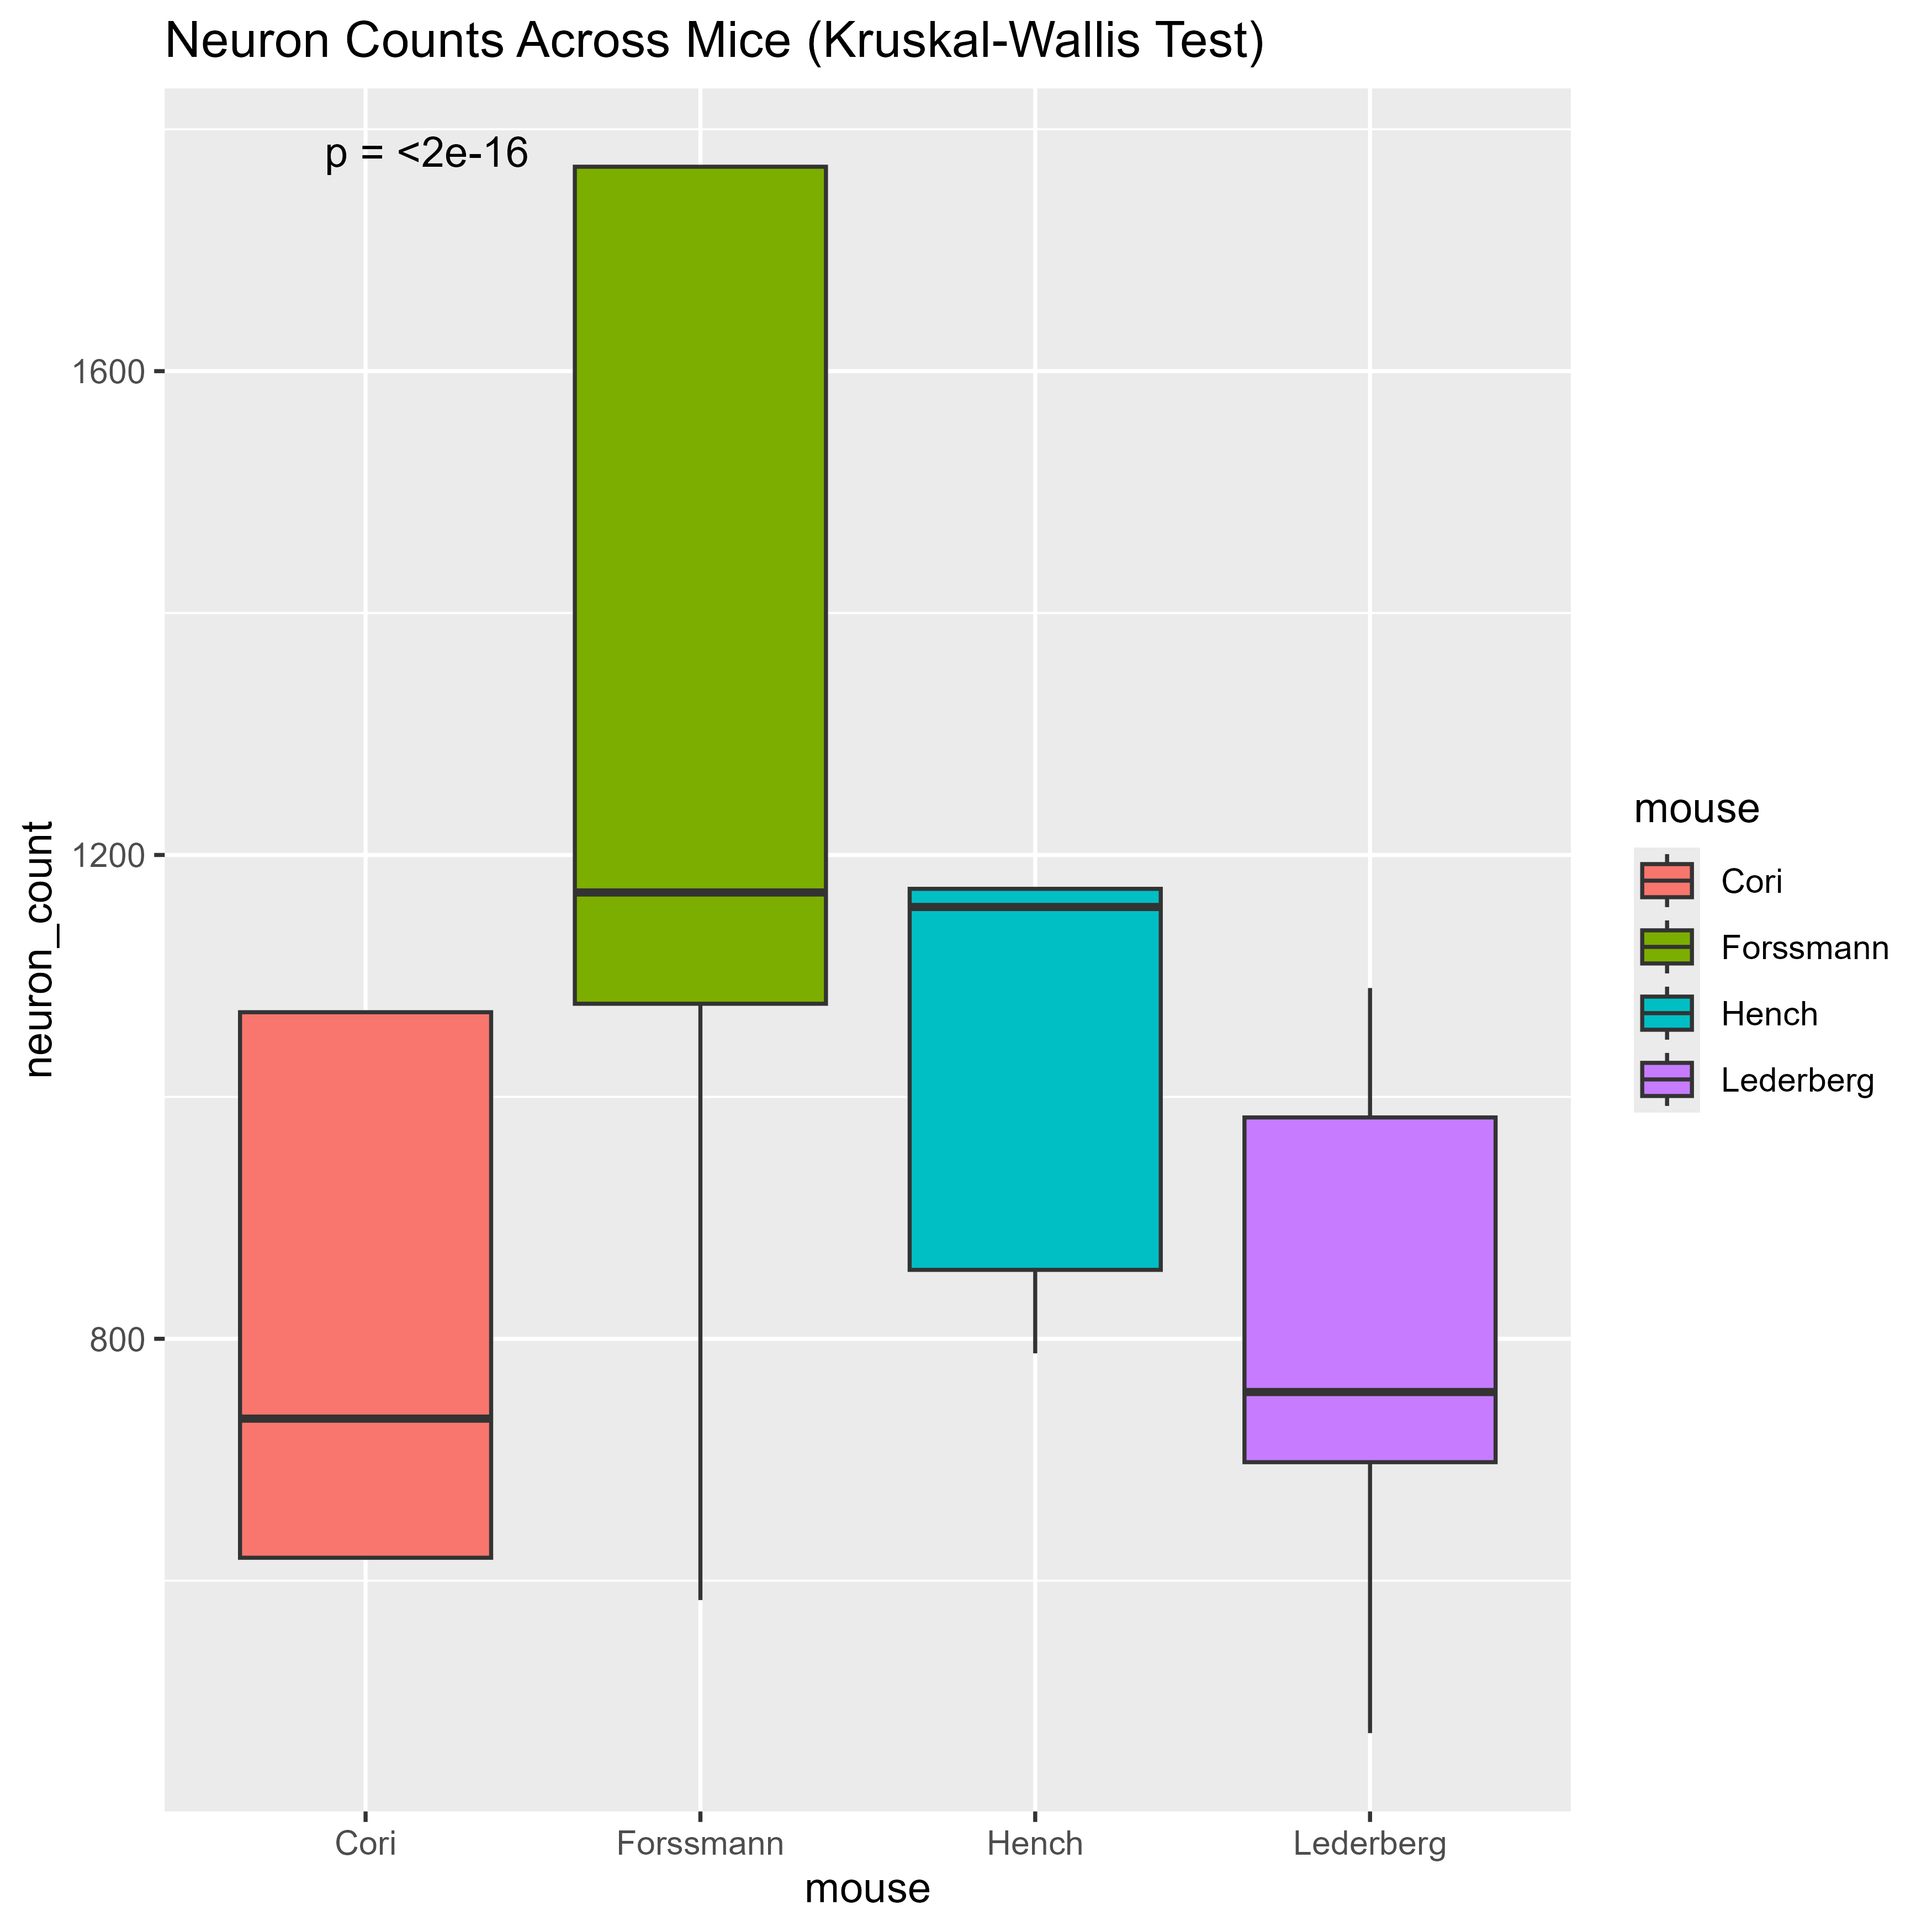
\includegraphics[scale=0.27]{Pics/012}\label{fig:1.12}
			\caption{The Neuron Count}
		\end{minipage}
		\begin{minipage}[t]{0.48\textwidth}
			\centering
			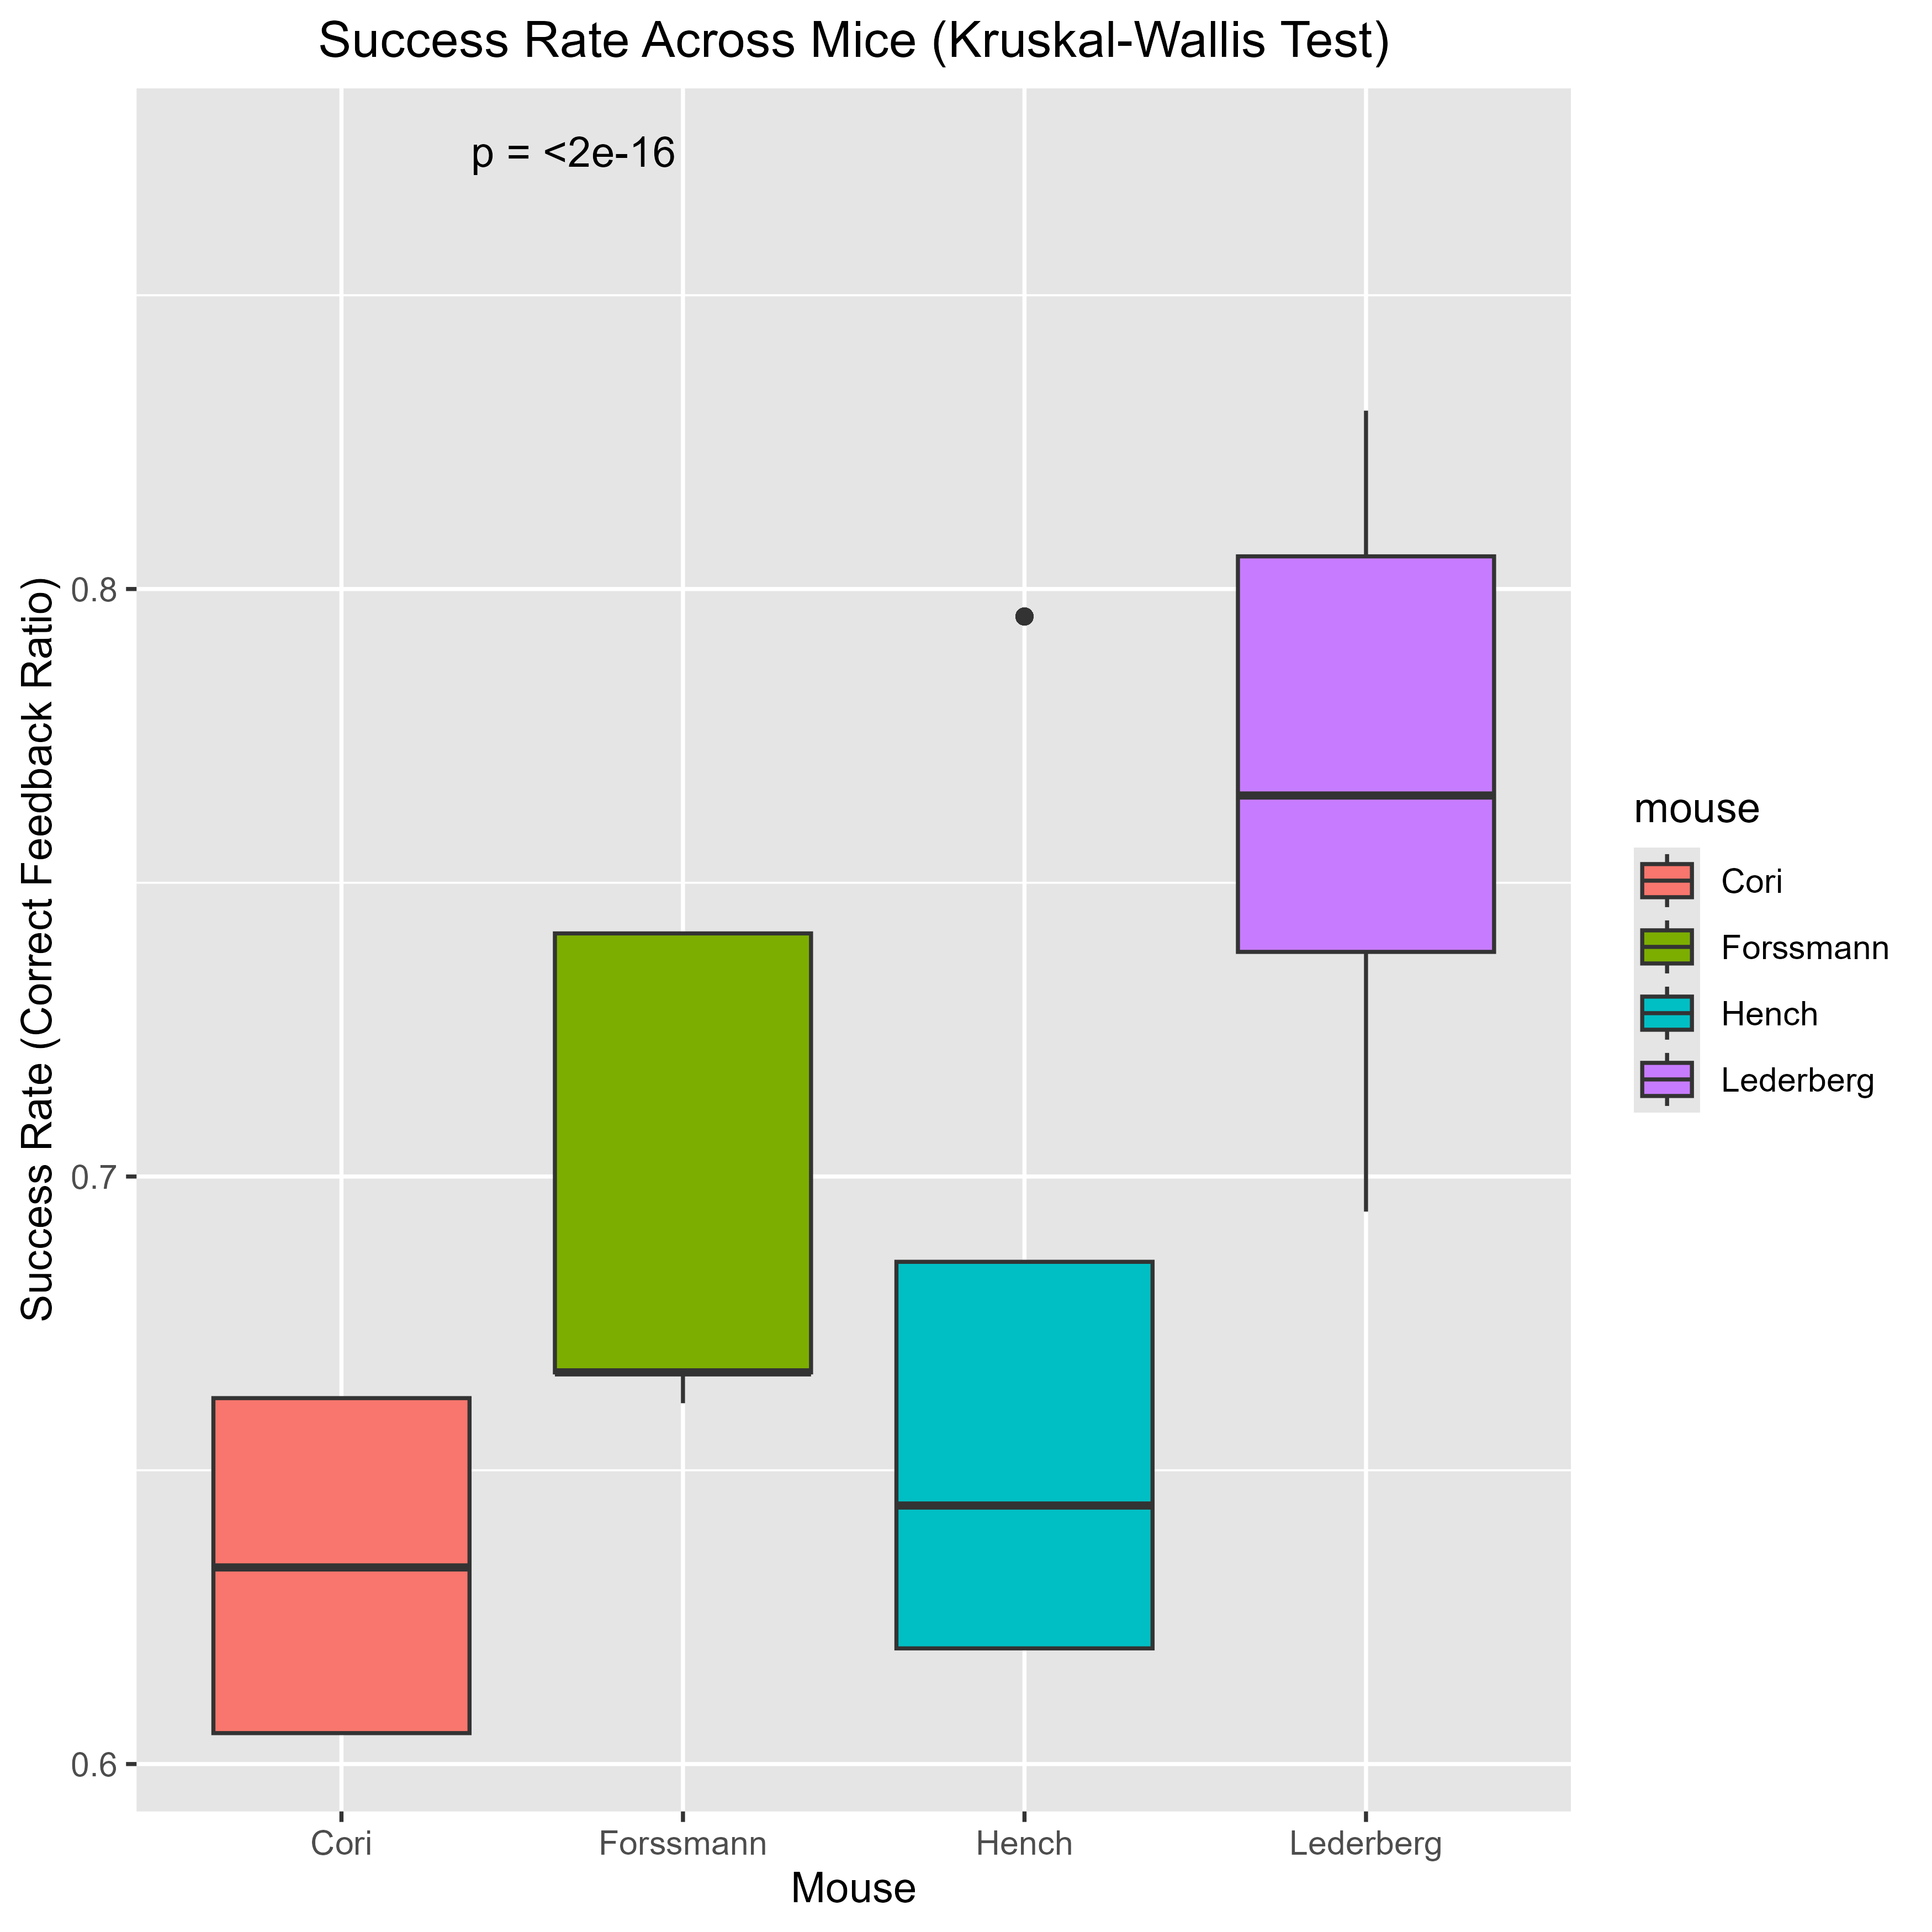
\includegraphics[scale=0.27]{Pics/015}\label{fig:1.15}
			\caption{The Success Rate}
		\end{minipage}
	\end{figure}
	\par Also, the box plots for the mean left/right contrast are also shown below.
	\begin{figure}[htbp]
		\centering
		\begin{minipage}[t]{0.48\textwidth}
			\centering
			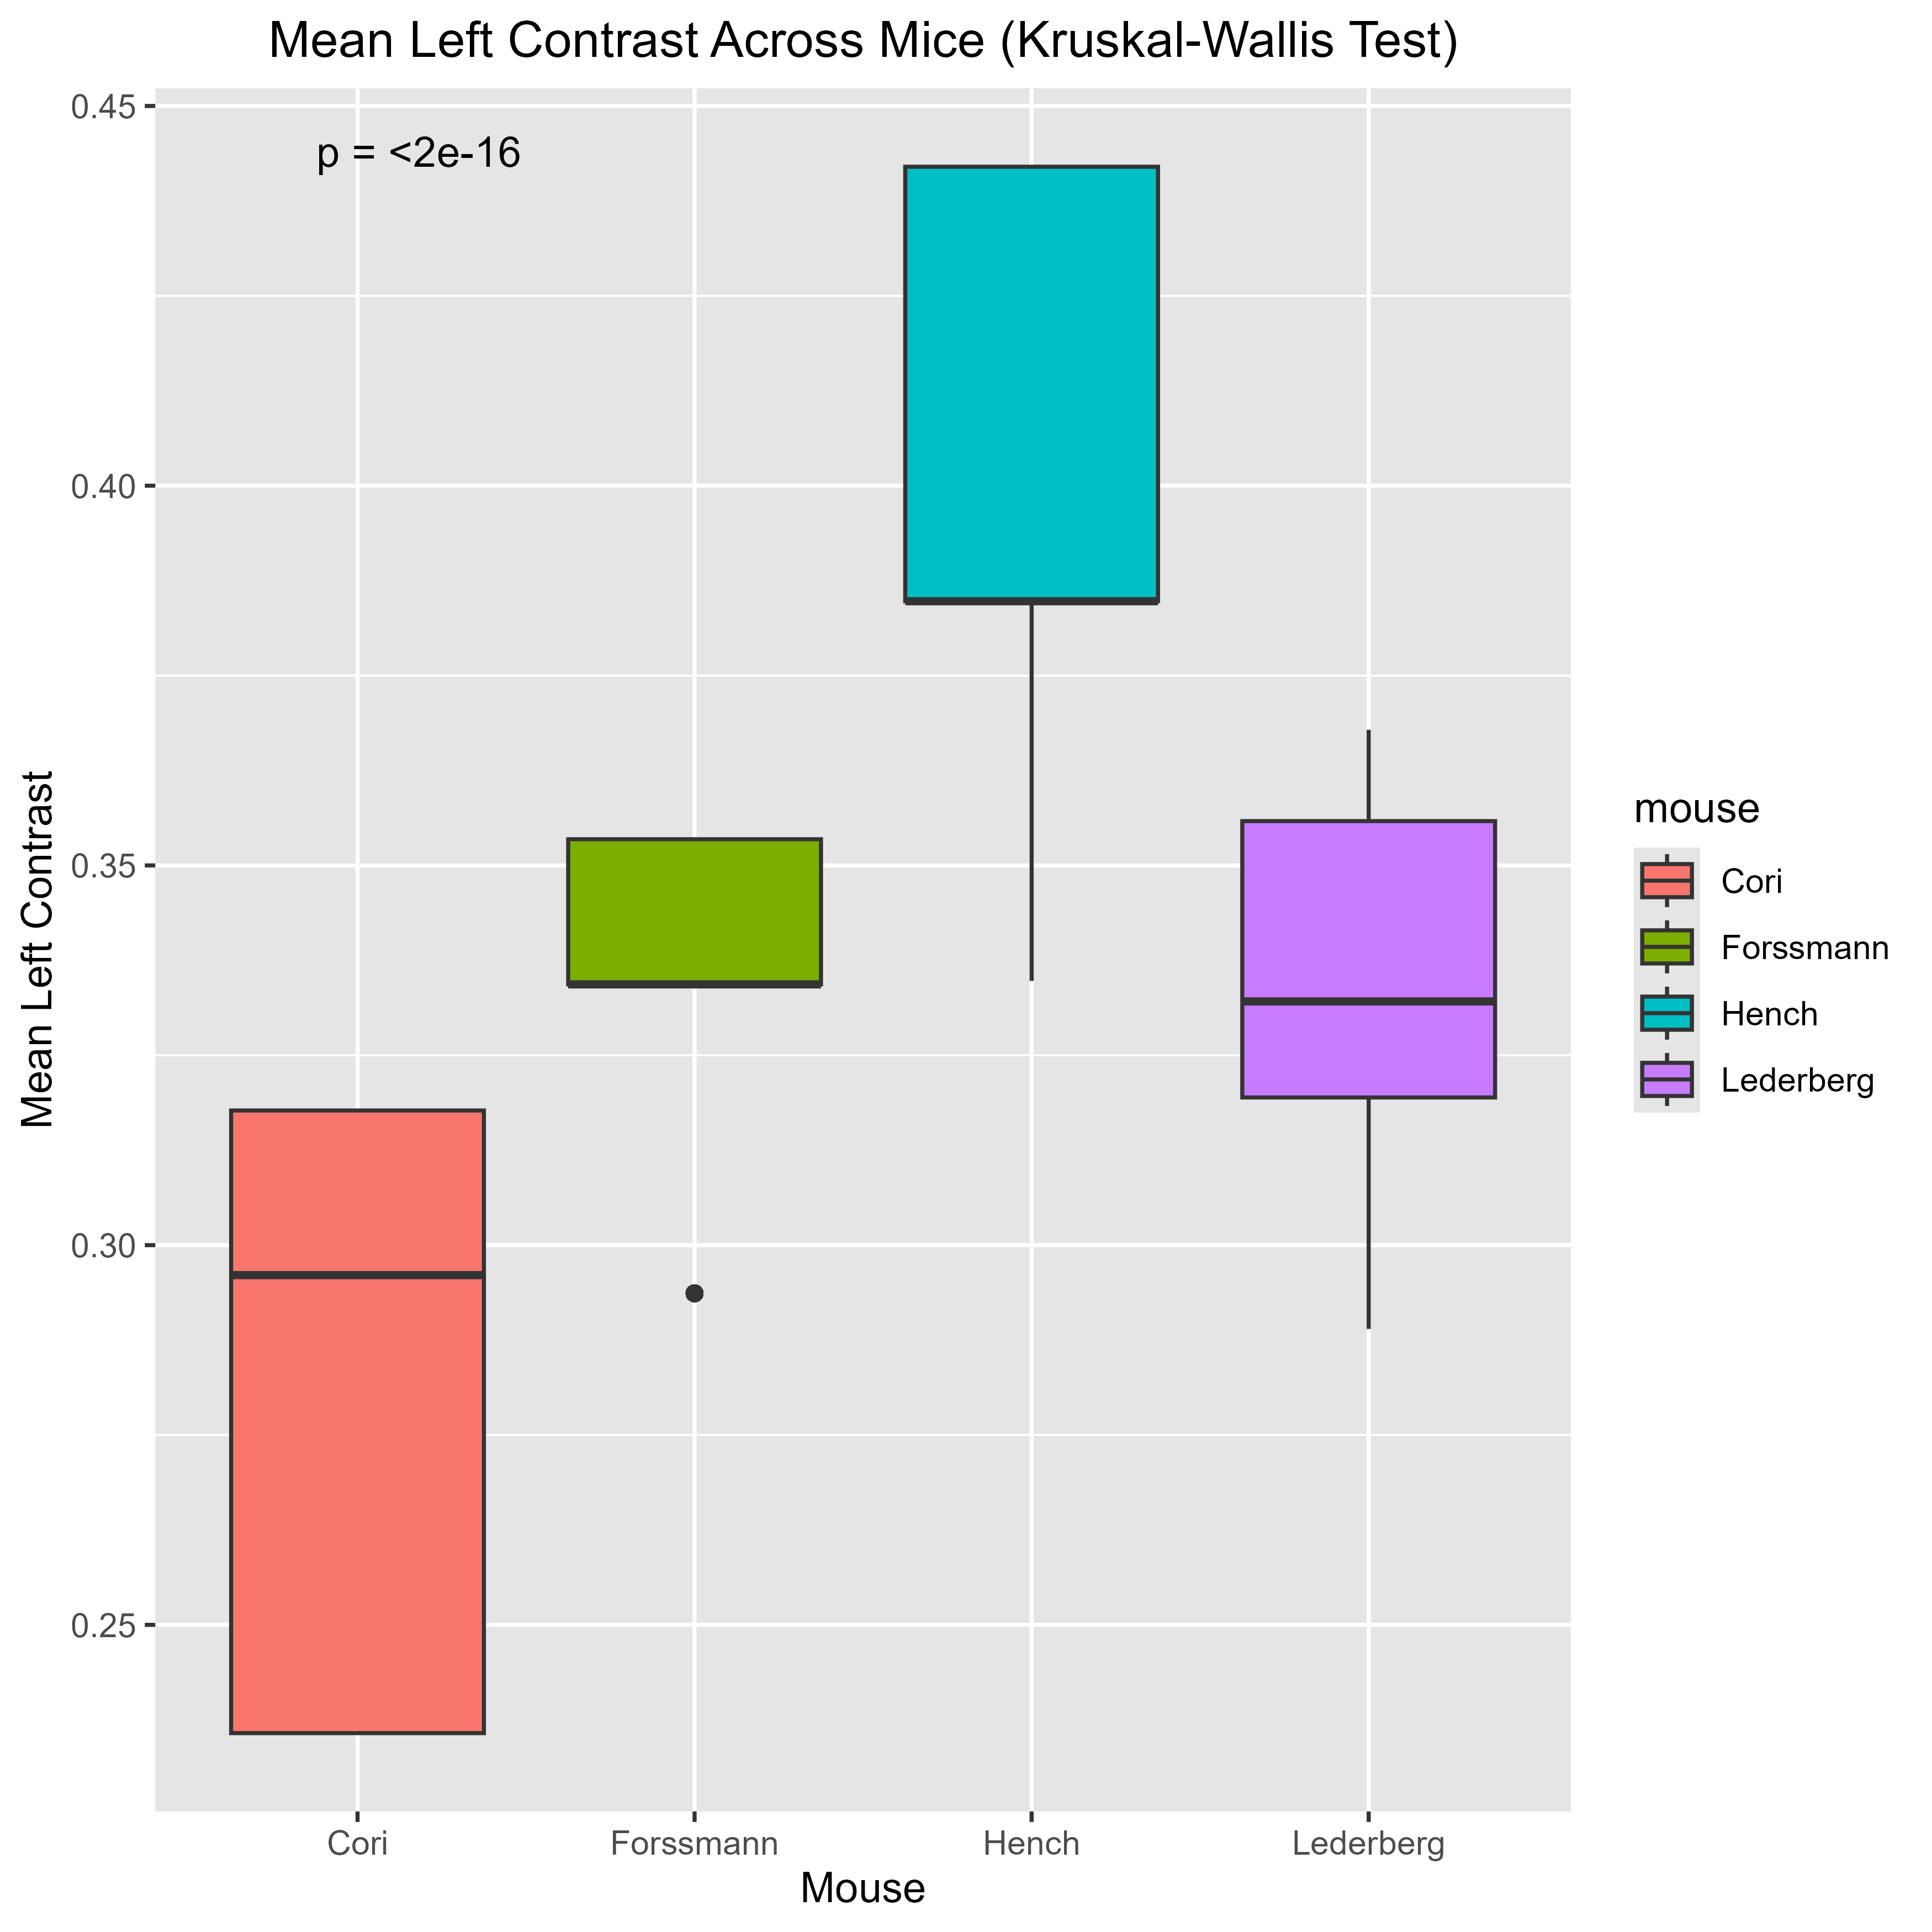
\includegraphics[scale=0.27]{Pics/013}\label{fig:1.13}
			\caption{The Mean Left Contrast}
		\end{minipage}
		\begin{minipage}[t]{0.48\textwidth}
			\centering
			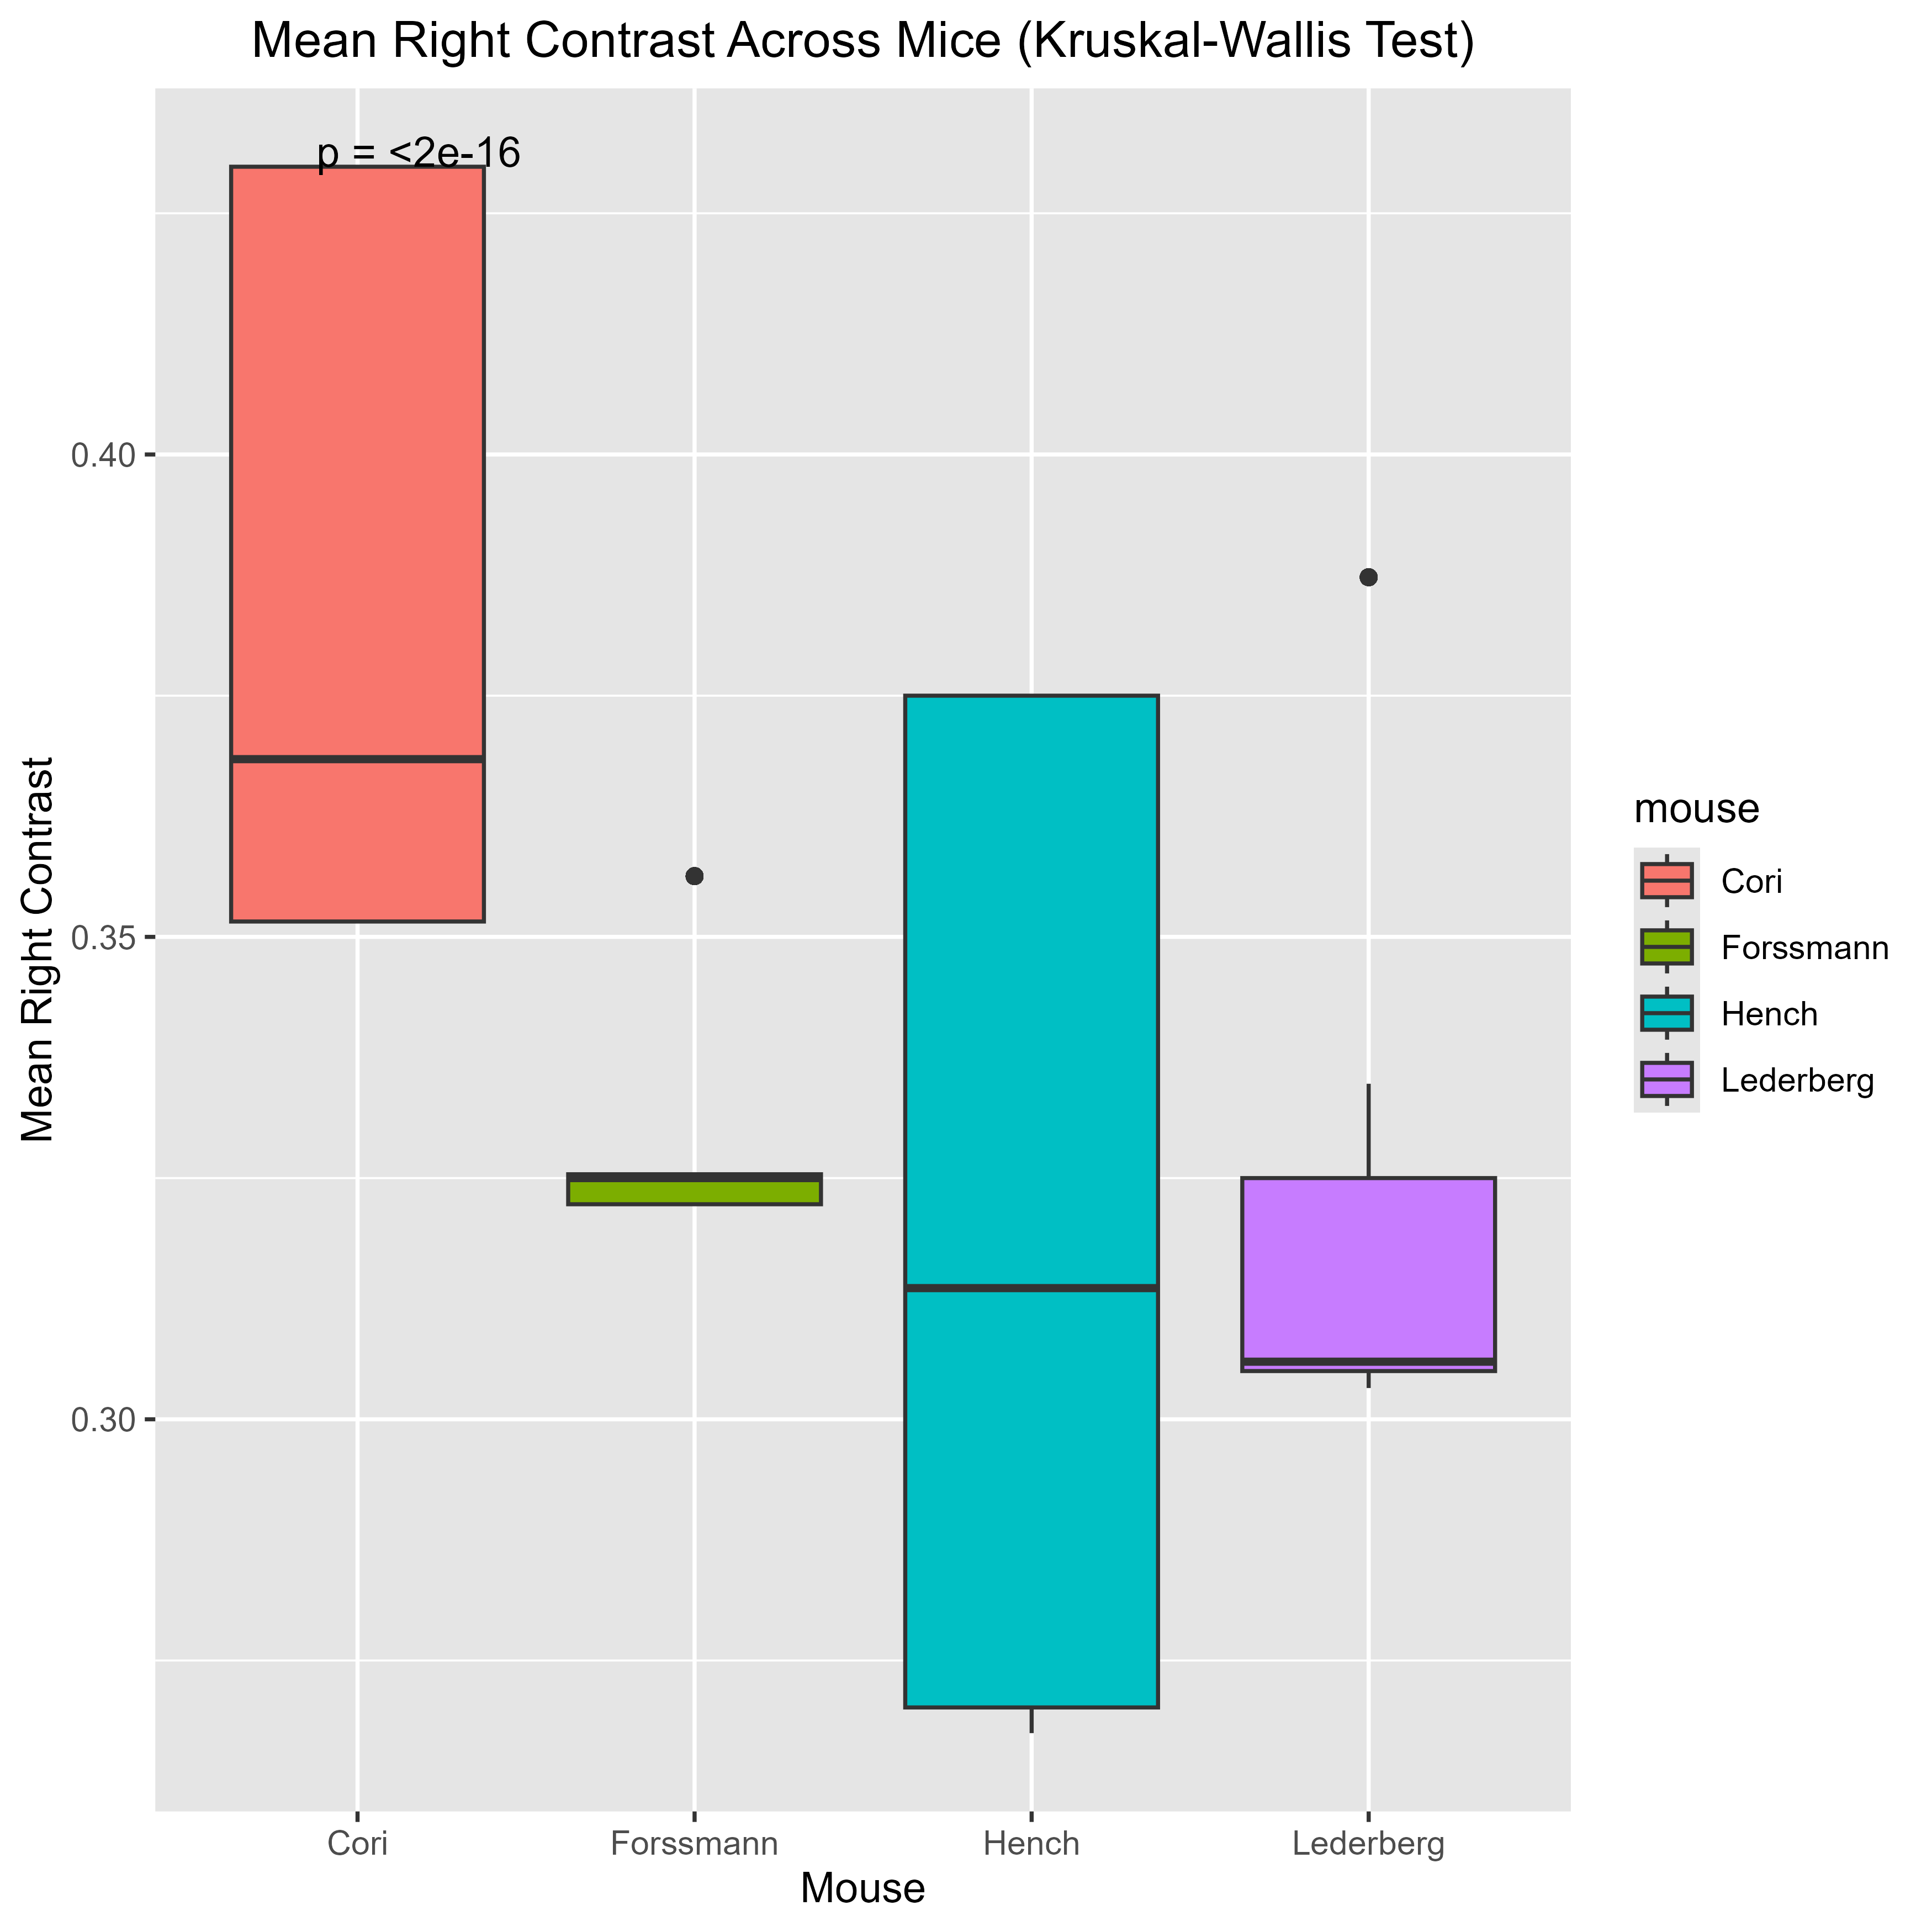
\includegraphics[scale=0.27]{Pics/014}\label{fig:1.14}
			\caption{The Mean Right Contrast}
		\end{minipage}
	\end{figure}
	\clearpage
	\par As we can see, there are clear gap between medians of them four. Concluding with the preliminary results, we now perform a K-W test on the data.
	\subsubsection{Kruskal-Wallis Test}
	\par The Kruskal-Wallis (KW) test we performed aims to assess \textbf{the homogeneity of neuron counts, mean left contrast, mean right contrast, and the correct feedback ratio across four mice (Forssmann, Hench, Lederberg, Cori)}. The results shown below.
	\begin{framed}
		\begin{verbatim}
			$mean_left_contrast
			
			Kruskal-Wallis rank sum test
			
			data:  mean_left_contrast by mouse
			Kruskal-Wallis chi-squared = 9049.4, df = 3, p-value < 2.2e-16
			
			
			$mean_right_contrast
			
			Kruskal-Wallis rank sum test
			
			data:  mean_right_contrast by mouse
			Kruskal-Wallis chi-squared = 4807.9, df = 3, p-value < 2.2e-16
			
			
			$neuron_count
			
			Kruskal-Wallis rank sum test
			
			data:  neuron_count by mouse
			Kruskal-Wallis chi-squared = 6081.6, df = 3, p-value < 2.2e-16
			
			
			$correct_feedback_ratio
			
			Kruskal-Wallis rank sum test
			
			data:  correct_feedback_ratio by mouse
			Kruskal-Wallis chi-squared = 9488, df = 3, p-value < 2.2e-16
		\end{verbatim}
	\end{framed}
	\clearpage
	\textbf{Analysis of Kruskal-Wallis Test Results:}
	\par Group by mouse, the K-W test was conducted to examine the differences across multiple experimental sessions for the following four key perspectives:
	\begin{itemize}
		\item [1)] Mean Left Contrast:
		\par As we can see, the $\chi^2$ value is $9049.4$ with $df = 3$ and $p-$value less than $2.2\times 10^{-16}$. Then we can be sure than there \textbf{is a highly significant difference }($p<2.2\times 10^{-16}$) in the mean left contrast among mice. This suggests left stimulus conditions were not balanced across mice, potentially due to inconsistent stimulus parameter settings in the experimental design.
		\item [2)] Mean Right Contrast:
		\par In the same way, the $\chi^2$ value is $4807.9$ with $df = 3$ and $p-$value less than $2.2\times 10^{-16}$ as well. Although the magnitude of this difference is smaller than the Mean Left Contrast, it's enough to say the right stimulus conditions were not balanced across mice as well.
		\item [3)] Neuron Count:
		\par As the box plot shown before, we have already noticed that there's a huge difference among mice. With the K-W test results, we found the $\chi^2$ value is $6081.6$ with $df = 3$ and the $p-$value less than $2.2\times 10^{-16}$. This variability reflects recording quality or biological differences among individual mice.
		\item [4)] Correct Feedback Ratio:
		\par The outcomes also have a highly significant difference with $\chi^2 = 9488$ and the same less enough $p-$value, indicating substantial variability in task performance. These differences of outcomes could be attributed to differences in learning ability, motivation levels, or inconsistencies in experimental conditions.
	\end{itemize}
	\par Above all, the Kruskal-Wallis test results reveal significant differences across mice for all four key metrics analyzed: Mean Left Contrast, Mean Right Contrast, Neuron Count, and Correct Feedback Ratio with all $p-$values less than $2.2\times 10^{-16}$. These findings suggest substantial variability in both experimental conditions and individual mouse performance, which may significantly impact the interpretability and generalizability of the results.
	\par Moreover, in the predictive model that we are going to build, the KW Test results suggest that we need to take the followings into consideration:
	\begin{itemize}
		\item [1)] Standardization and Normalization plays a crucial role in the data integration.
		\item [2)] Model Generalization: Given the variability across mice, it is important to validate models using \textbf{cross-validation} techniques that account for individual differences.
	\end{itemize}
	\clearpage
	\section{Data Integration}
	\par In this part, we need to propose an approach to combine data across trials, for the convenience to build up a predictive model in part 3. It is the bridge for data analysis and predict modeling. By standardizing the neural activity data and extracting key features through \textbf{PCA}, we create a consistent representation of neural patterns across sessions. The above data integration process ensures that the final dataset captures both within-session and cross-session variability, providing a robust foundation for developing predictive models in Part 3. The main tasks are constructed as follows:
	\begin{table}[htbp]
		\centering
		\begin{tabular}{p{4cm}p{10cm}}
			\toprule
			\textbf{Task} & \textbf{Description} \\
			\midrule
			Data Standardization & Normalize neural activity data across sessions\\
			Feature Extraction & Use PCA to reduce dimensionality\\
			Cross-Session Feature Alignment & Identify common patterns and align features across different sessions\\
			Data Integration & Combine data from all sessions\\
			\bottomrule
		\end{tabular}
	\end{table}
	\par In the last two subsections, we introduced new statistic method applied in Biology, named the \textbf{Harmony Algorithm}, which adjusted for batch effects (i.e. Session-Specific recording conditions).
	\subsection{Data Standardization}
	\par To enable cross-session comparability and model generalizability, we performed session-wise standardization on neural activity data. For each session, raw spike trains were aggregated into interpretable features \textbf{by averaging firing rates across brain areas (e.g., VISp, ACA) and time windows (0–0.1s, 0.1–0.2s, 0.2–0.3s, 0.3–0.4s)}. These features were then standardized within each session using Z-score normalization (with mean $= 0$, SD $= 1$) to eliminate baseline variations caused by session-specific recording conditions or biological variability. Part of the results are shown below.(Window 1 to 4 represents the time 0-0.1s to 0.3-0.4s respectively).
	\begin{framed}
		\begin{verbatim}
			VISa_window1_mean VISa_window2_mean VISa_window3_mean VISa_window4_mean
			1     -6.304825e-17      1.538807e-16      1.504693e-17     -7.965557e-17
			root_window1_mean root_window2_mean root_window3_mean root_window4_mean
			1      1.211779e-16      1.575218e-16      1.566183e-16      2.004767e-16
			
			VISa_window1_sd VISa_window2_sd VISa_window3_sd VISa_window4_sd
			1               1               1               1               1
			root_window1_sd root_window2_sd root_window3_sd root_window4_sd
			1               1               1               1               1
		\end{verbatim}
	\end{framed}
	\subsection{Feature Extraction}
	\par In this sub-part, we aim to use PCA to reduce the high dimensional data and extract the principal components with the highest variance in the data. With the top $100$ PCs, we found they yields $82\%$ of the accumulated total variance, indicating that approximately half of the variability in the high-dimensional spatiotemporal features can be represented in this reduced subspace.
	\begin{figure}[htbp]
		\centering
		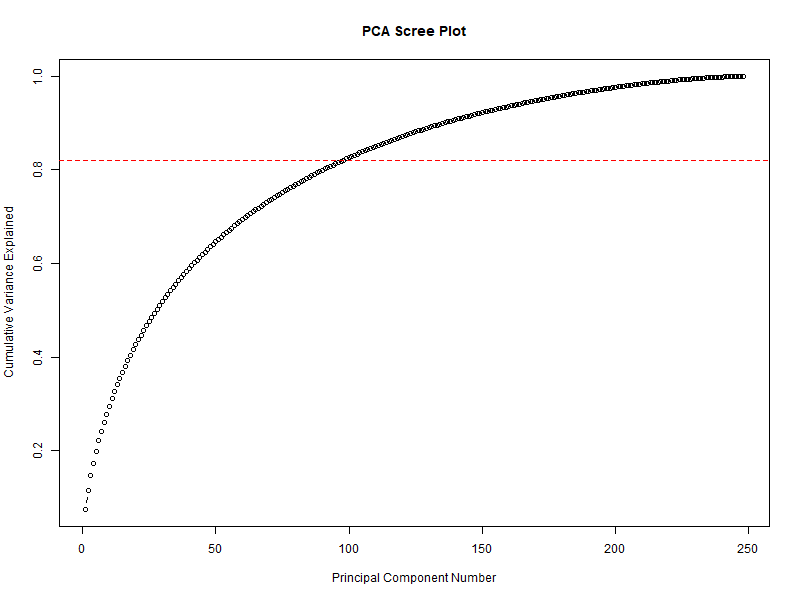
\includegraphics[scale = 0.4]{Pics/pca_scree_plot}
		\caption{PCA Scree Plot}
		\label{fig:pcascreeplot}
	\end{figure}
	
	\par Moreover, the MSE between the original standardized data and the reconstructed data using top $30$ PCs is \textbf{0.02703899}, suggesting relatively faithful preservation of the original neural activity patterns despite significant dimensionality reduction.
		\begin{framed}
		\begin{verbatim}
			MSE = 0.02703899 
		\end{verbatim}
	\end{framed}
	\clearpage
	\subsection{Cross-Session Feature Alignment with Harmony}
	\par For harmonizing data across sessions, the Harmony Algorithm was employed. This method adjusted for batch effects, which is exactly dealing with the session-specific recording conditions by aligning the distribution of PCs across sessions while preserving biologically meaningful signals (e.g., stimulus-response relationships). Post-alignment visualization confirmed reduced session-driven clustering in the PC space, enhancing cross-session comparability.
	\par After coding, we got the following graphs below:
		\begin{figure}[htbp]
		\centering
		\begin{minipage}[t]{0.48\textwidth}
			\centering
			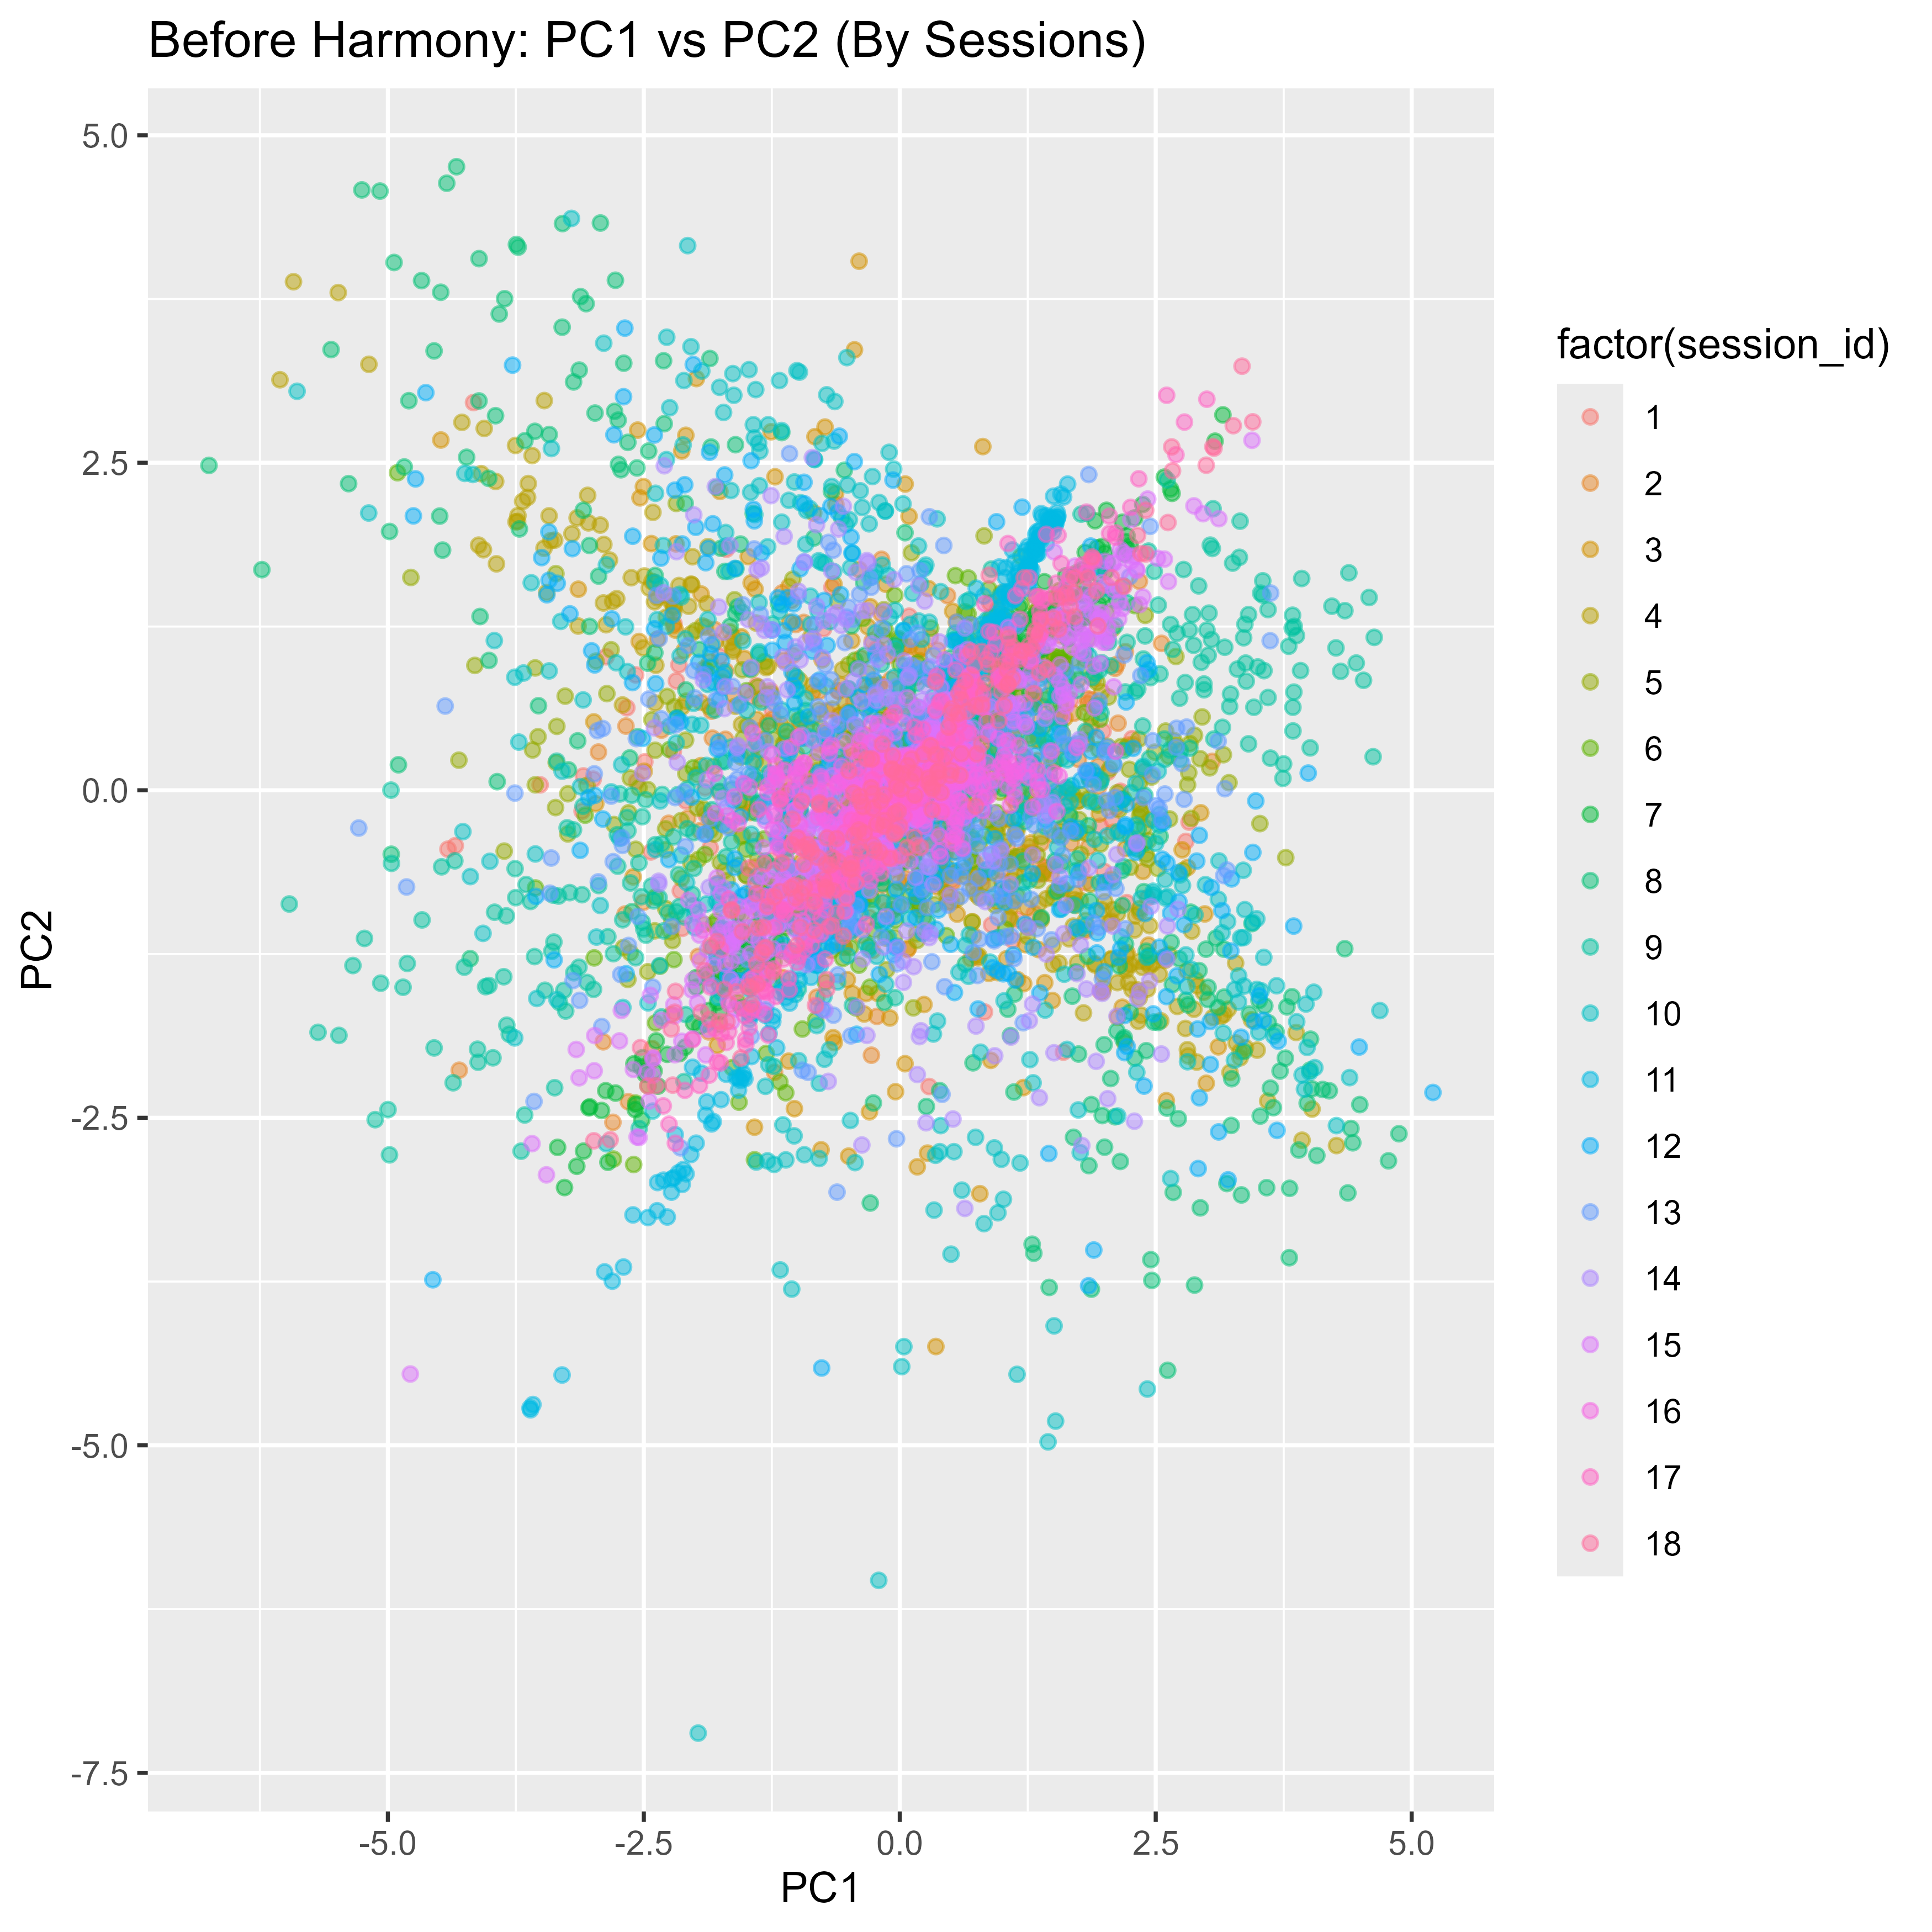
\includegraphics[scale=0.4]{Pics/15}\label{fig:1.17}
			\caption{PC1 vs PC2 before Harmony}
		\end{minipage}
		\begin{minipage}[t]{0.48\textwidth}
			\centering
			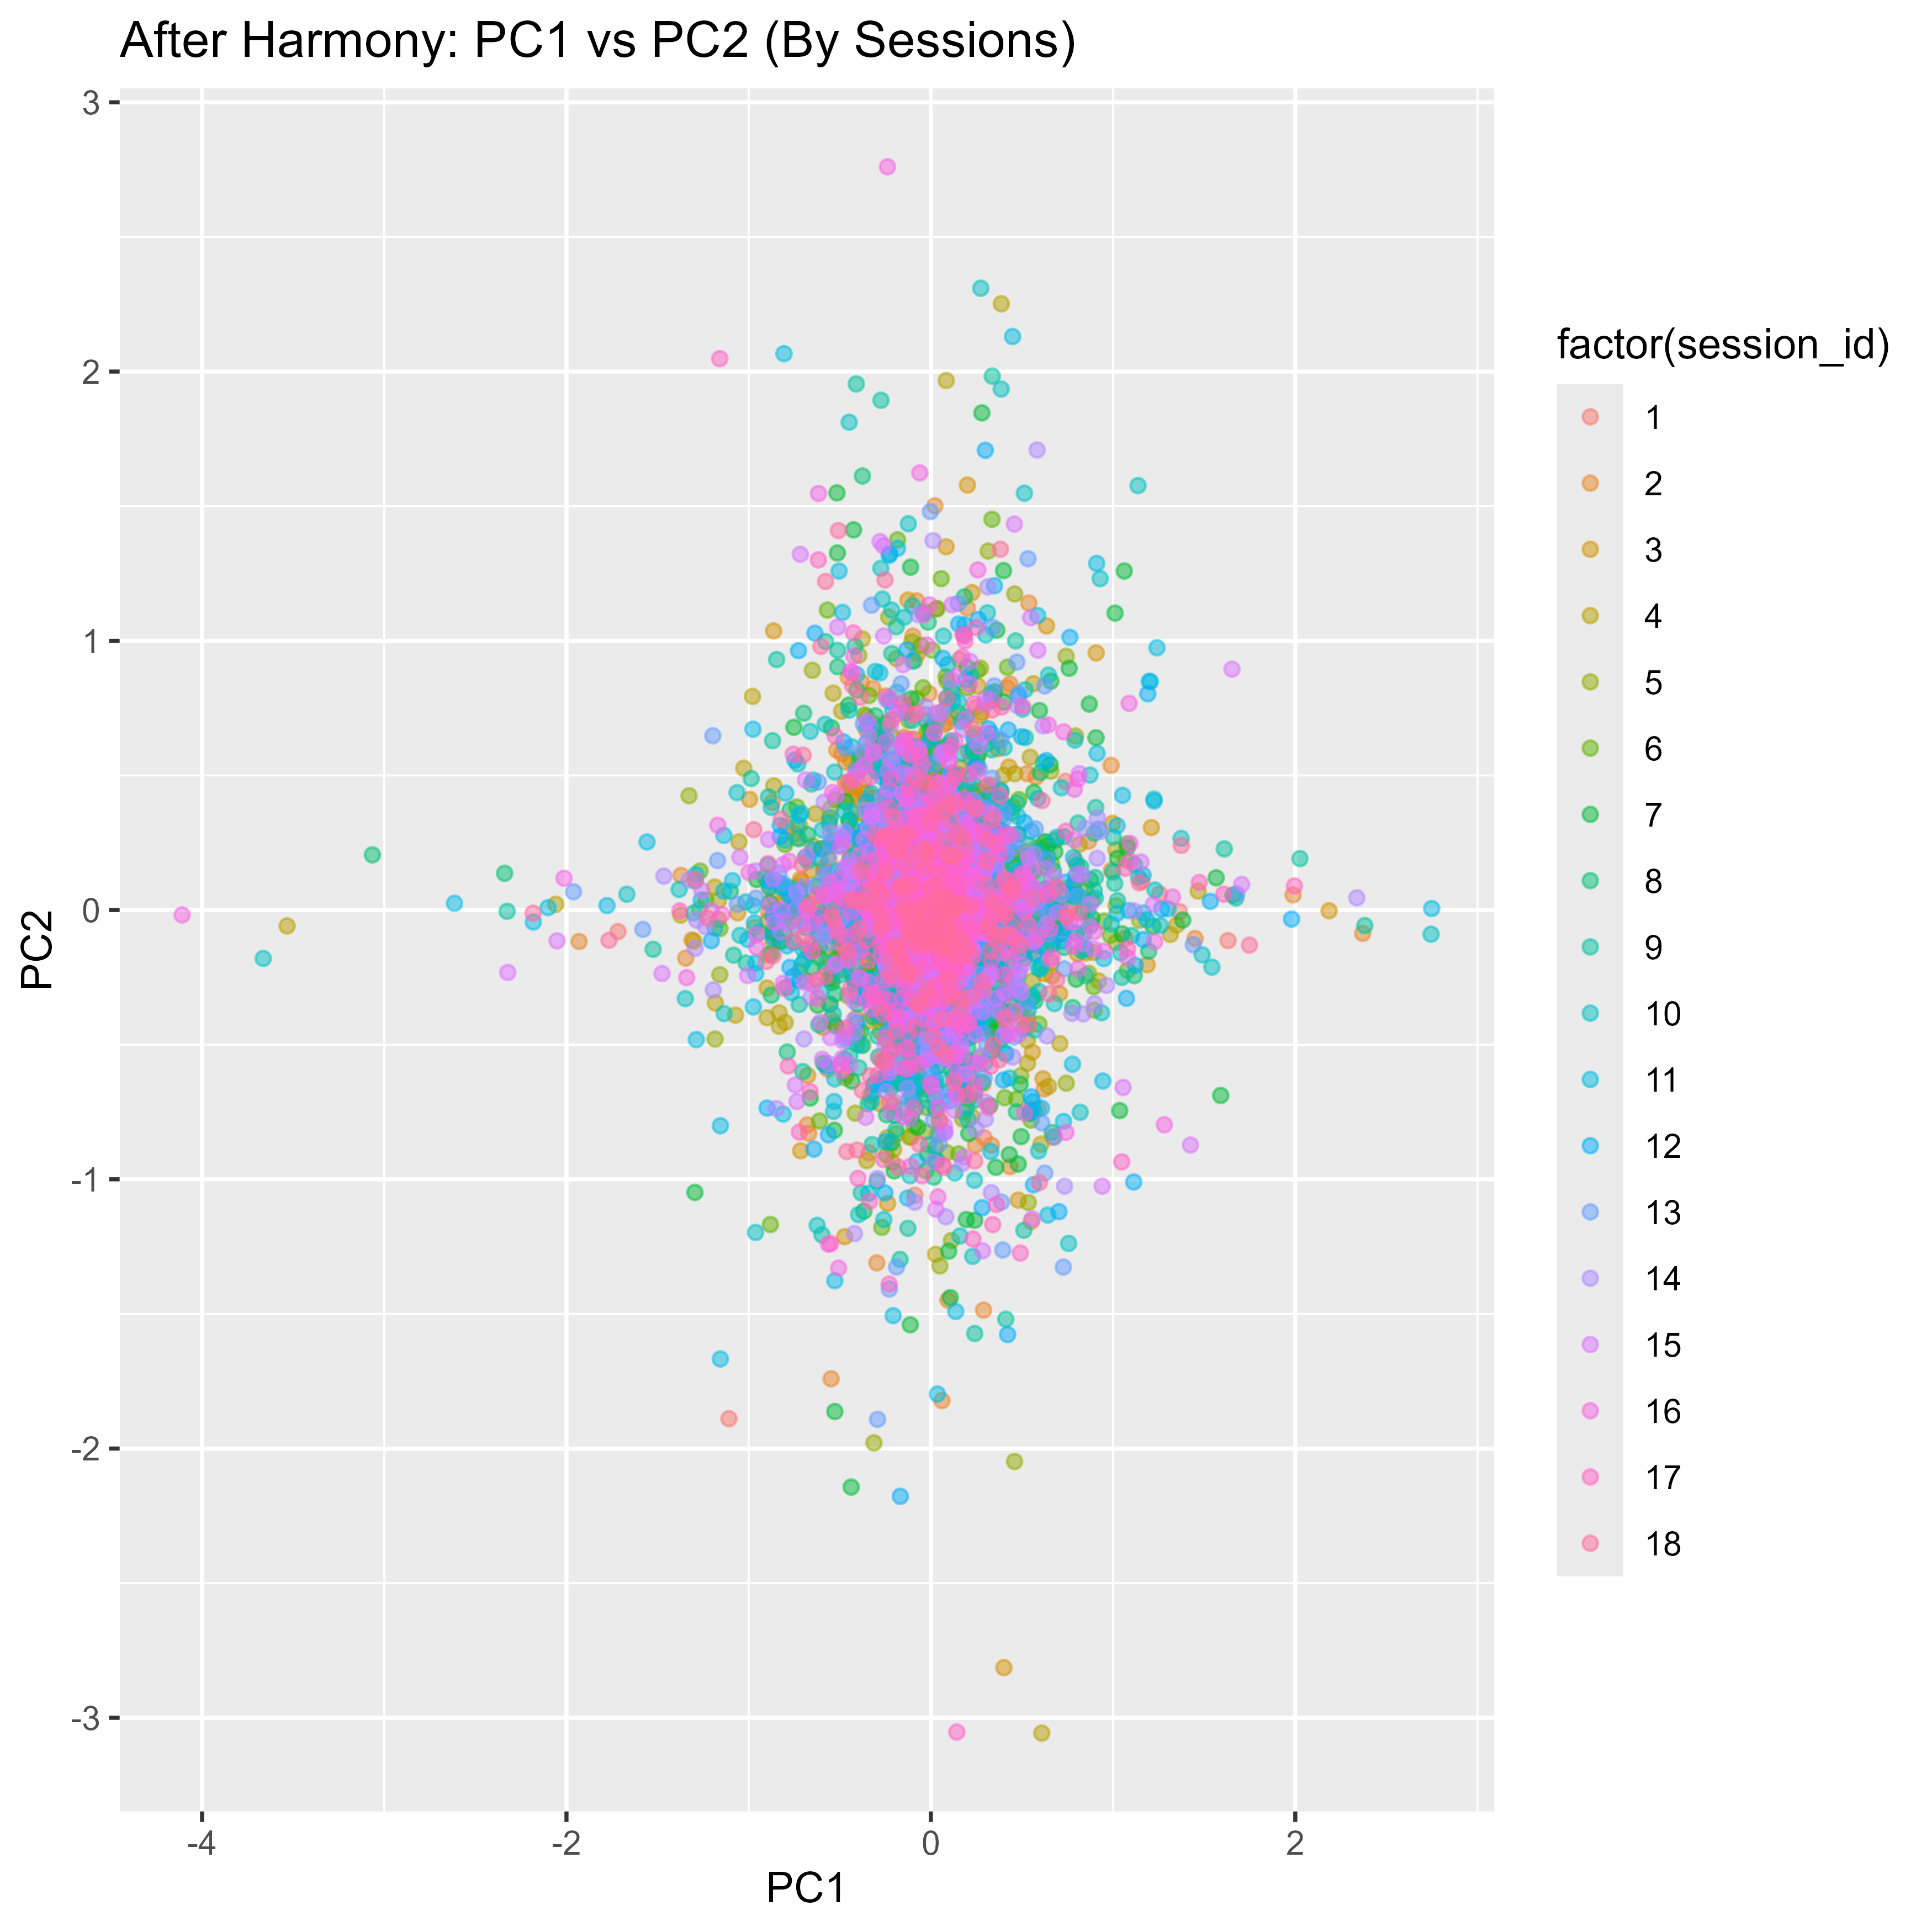
\includegraphics[scale=0.4]{Pics/16}\label{fig:1.16}
			\caption{PC1 vs PC2 after Harmony}
		\end{minipage}
	\end{figure}
	\subsection{Data Integration and Factor Conversion}
	\par In the final section of part 2, we let the harmonized dataset integrated into a unified proper structure, with  left contrast and right contrast, and the behavioral outcomes (feedback: $1$ for success and $-1$ for failure). Also, we take the categorical variables like session\_id and mouse\_name encoded as factors and put them into the unified structure as well, ensuring handling the predictive model in the next part properly.
	\par The final integrated dataset balances dimensionality reduction, batch correction, and interpretability, providing a robust foundation for training generalized classification models.
	\clearpage
	\section{Model Training and Prediction}
	\par Now, we dive into the part for predictive modeling. We already had the standardized, PCA-reduced, and Harmony-integrated data into training and test sets. The prediction set consisted of 100 randomly selected samples from session1 and session18, respectively. 
	\par We employed three machine learning models for prediction, including LASSO regression, K-Nearest Neighbors (KNN), and Logistic Regression. In the preliminary results of the LASSO model, we identified \textbf{a severe class imbalance issue}, which led to the model's inability to predict the minority class (-1) effectively. Specifically, the confusion matrix showed that all predictions for the minority class were 0, while the majority class (1) achieved high prediction accuracy. However, the overall model's Kappa value was 0, indicating that the model failed to effectively distinguish between the two classes.
	\par To address the class imbalance issue, we applied the Synthetic Minority Over-sampling Technique (SMOTE) to the training data. After SMOTE processing, the number of minority class samples in the training set increased to 4158, while the majority class samples numbered 3365, resulting in a more balanced ratio between the two classes. 
	\par Subsequently, we retrained and predicted using the LASSO, KNN, and Logistic Regression models. However, the performance of the LASSO model remained suboptimal. Although the class imbalance issue was mitigated, the model's predictive capability did not improve significantly. The KNN model showed some improvement after SMOTE processing, but its F1 Score was only 0.147, indicating that the model's predictive ability for the minority class was still weak.
	\par In further analysis, we observed that the KNN model's confusion matrix after SMOTE processing showed high prediction accuracy for the majority class (1), but its ability to predict the minority class (-1) remained insufficient. Specifically, the KNN model achieved an F1 Score of 0.404878, which, although improved compared to the pre-SMOTE results, still fell short of the desired level. The Logistic Regression model performed relatively better after SMOTE processing, with an F1 Score of 0.3754045, suggesting enhanced predictive capability on the balanced dataset, though there is still room for improvement.
	\par Finally, we attempted to use XGBoost combined with the SMOTE method for prediction. The XGBoost model demonstrated significantly better performance than the other models after SMOTE processing. Its confusion matrix revealed high prediction accuracy for the majority class (1), along with improved predictive capability for the minority class (-1). The XGBoost model achieved an F1 Score of 0.3743316 and an ROC-AUC value of 0.6068303, indicating that the model exhibited balanced predictive performance on the dataset and outperformed the other models in overall performance.
	\clearpage
	\subsection{LASSO}
	\par For the LASSO part, we trained the model with train set and found the best lambda (See the Fig below)
	\begin{figure}[htbp]
		\centering
		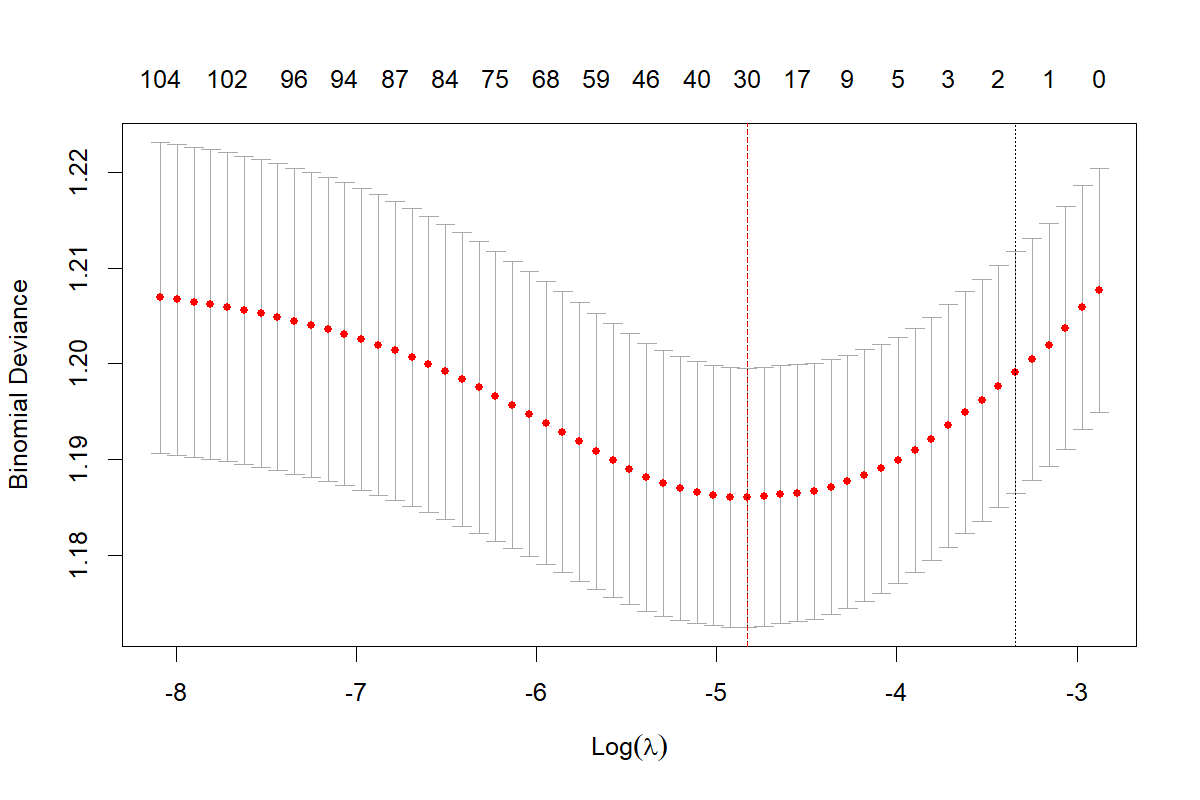
\includegraphics[scale = 0.5]{Pics/lasso_cv_plot}
		\caption{LASSO CV Plot}
		\label{fig:lassocvplot}
	\end{figure}
	\par And the best lambda turns out to be:
	$$\mbox{best\_lambda} = 0.00798771359450813.$$
	Then, we constructed the LASSO Model with the best lambda (lambda\_min) and predicted the predict set from session 1 and session 18. The Confusion Matrix and other results are shown below.
	\begin{framed}
		\begin{verbatim}
			Confusion Matrix and Statistics
			
			Reference
			Prediction  -1   1
			-1   0   0
			1   87 243
			
			Accuracy : 0.7364          
			95% CI : (0.6853, 0.7831)   
		\end{verbatim}
	\end{framed}
	\par As we can see, the results predicted all data to success $1$. Though the accuracy of the model is 0.7364, which is high enough, but it is identical to the no information rate (the accuracy achieved by always predicting the majority class). This indicates that the model's performance is \textbf{no better than random guessing} based on the majority class.
	\clearpage
	\par We then took a look at the distribution of training set and found:
		\begin{framed}
		\begin{verbatim}
			The training set distribution:
			y_train
			0    1 
			1386 3365 
			The predicting set distribution:
			y_test
			0   1 
			87 243      
		\end{verbatim}
	\end{framed}
	\par The results clearly indicate that the LASSO model struggles with the ​\textbf{class imbalance problem}. The model's inability to predict the minority class (-1) and its reliance on the majority class (1) for achieving accuracy suggest that the data distribution is heavily skewed. This imbalance leads to biased predictions, where the model prioritizes the majority class at the expense of the minority class.
	\par By searching and studying new method to address this issue, we found \textbf{SMOTE (Synthetic Minority Over-sampling Technique) }. It can generate synthetic samples of the minority class to balance the distribution, then improving the model's ability to learn and predict both classes more efficiently.
	\clearpage
	\subsection{SMOTE}
	\par We applied SMOTE Algorithm, having the result:
	\begin{framed}
		\begin{verbatim}
			y_train_balanced
			-1    1 
			4158 3365   
		\end{verbatim}
	\end{framed}
	Now with more confident, we tried to use LASSO with SMOTE once again, but also with an suboptimal result. Thus, we decided to apply other models.
	\subsection{KNN}
	\subsubsection{KNN without SMOTE}
	\par Firstly, we trained a KNN model with $k\in\{3,5,7,9,11,13,15\}$ as candidates. The package ``caret'' will help us to find out the best performed $k$ with $10$ folds.
	\par The result of KNN without SMOTE is shown below.
		\begin{framed}
		\begin{verbatim}
			Confusion Matrix and Statistics
			
			Reference
			Prediction  -1   1
			-1   8  14
			1   79 229
			
			Accuracy : 0.7182          
			95% CI : (0.6663, 0.7661)
		\end{verbatim}
	\end{framed}
	The confusion matrix is also visualized below.
	\begin{figure}[htbp]
		\centering
		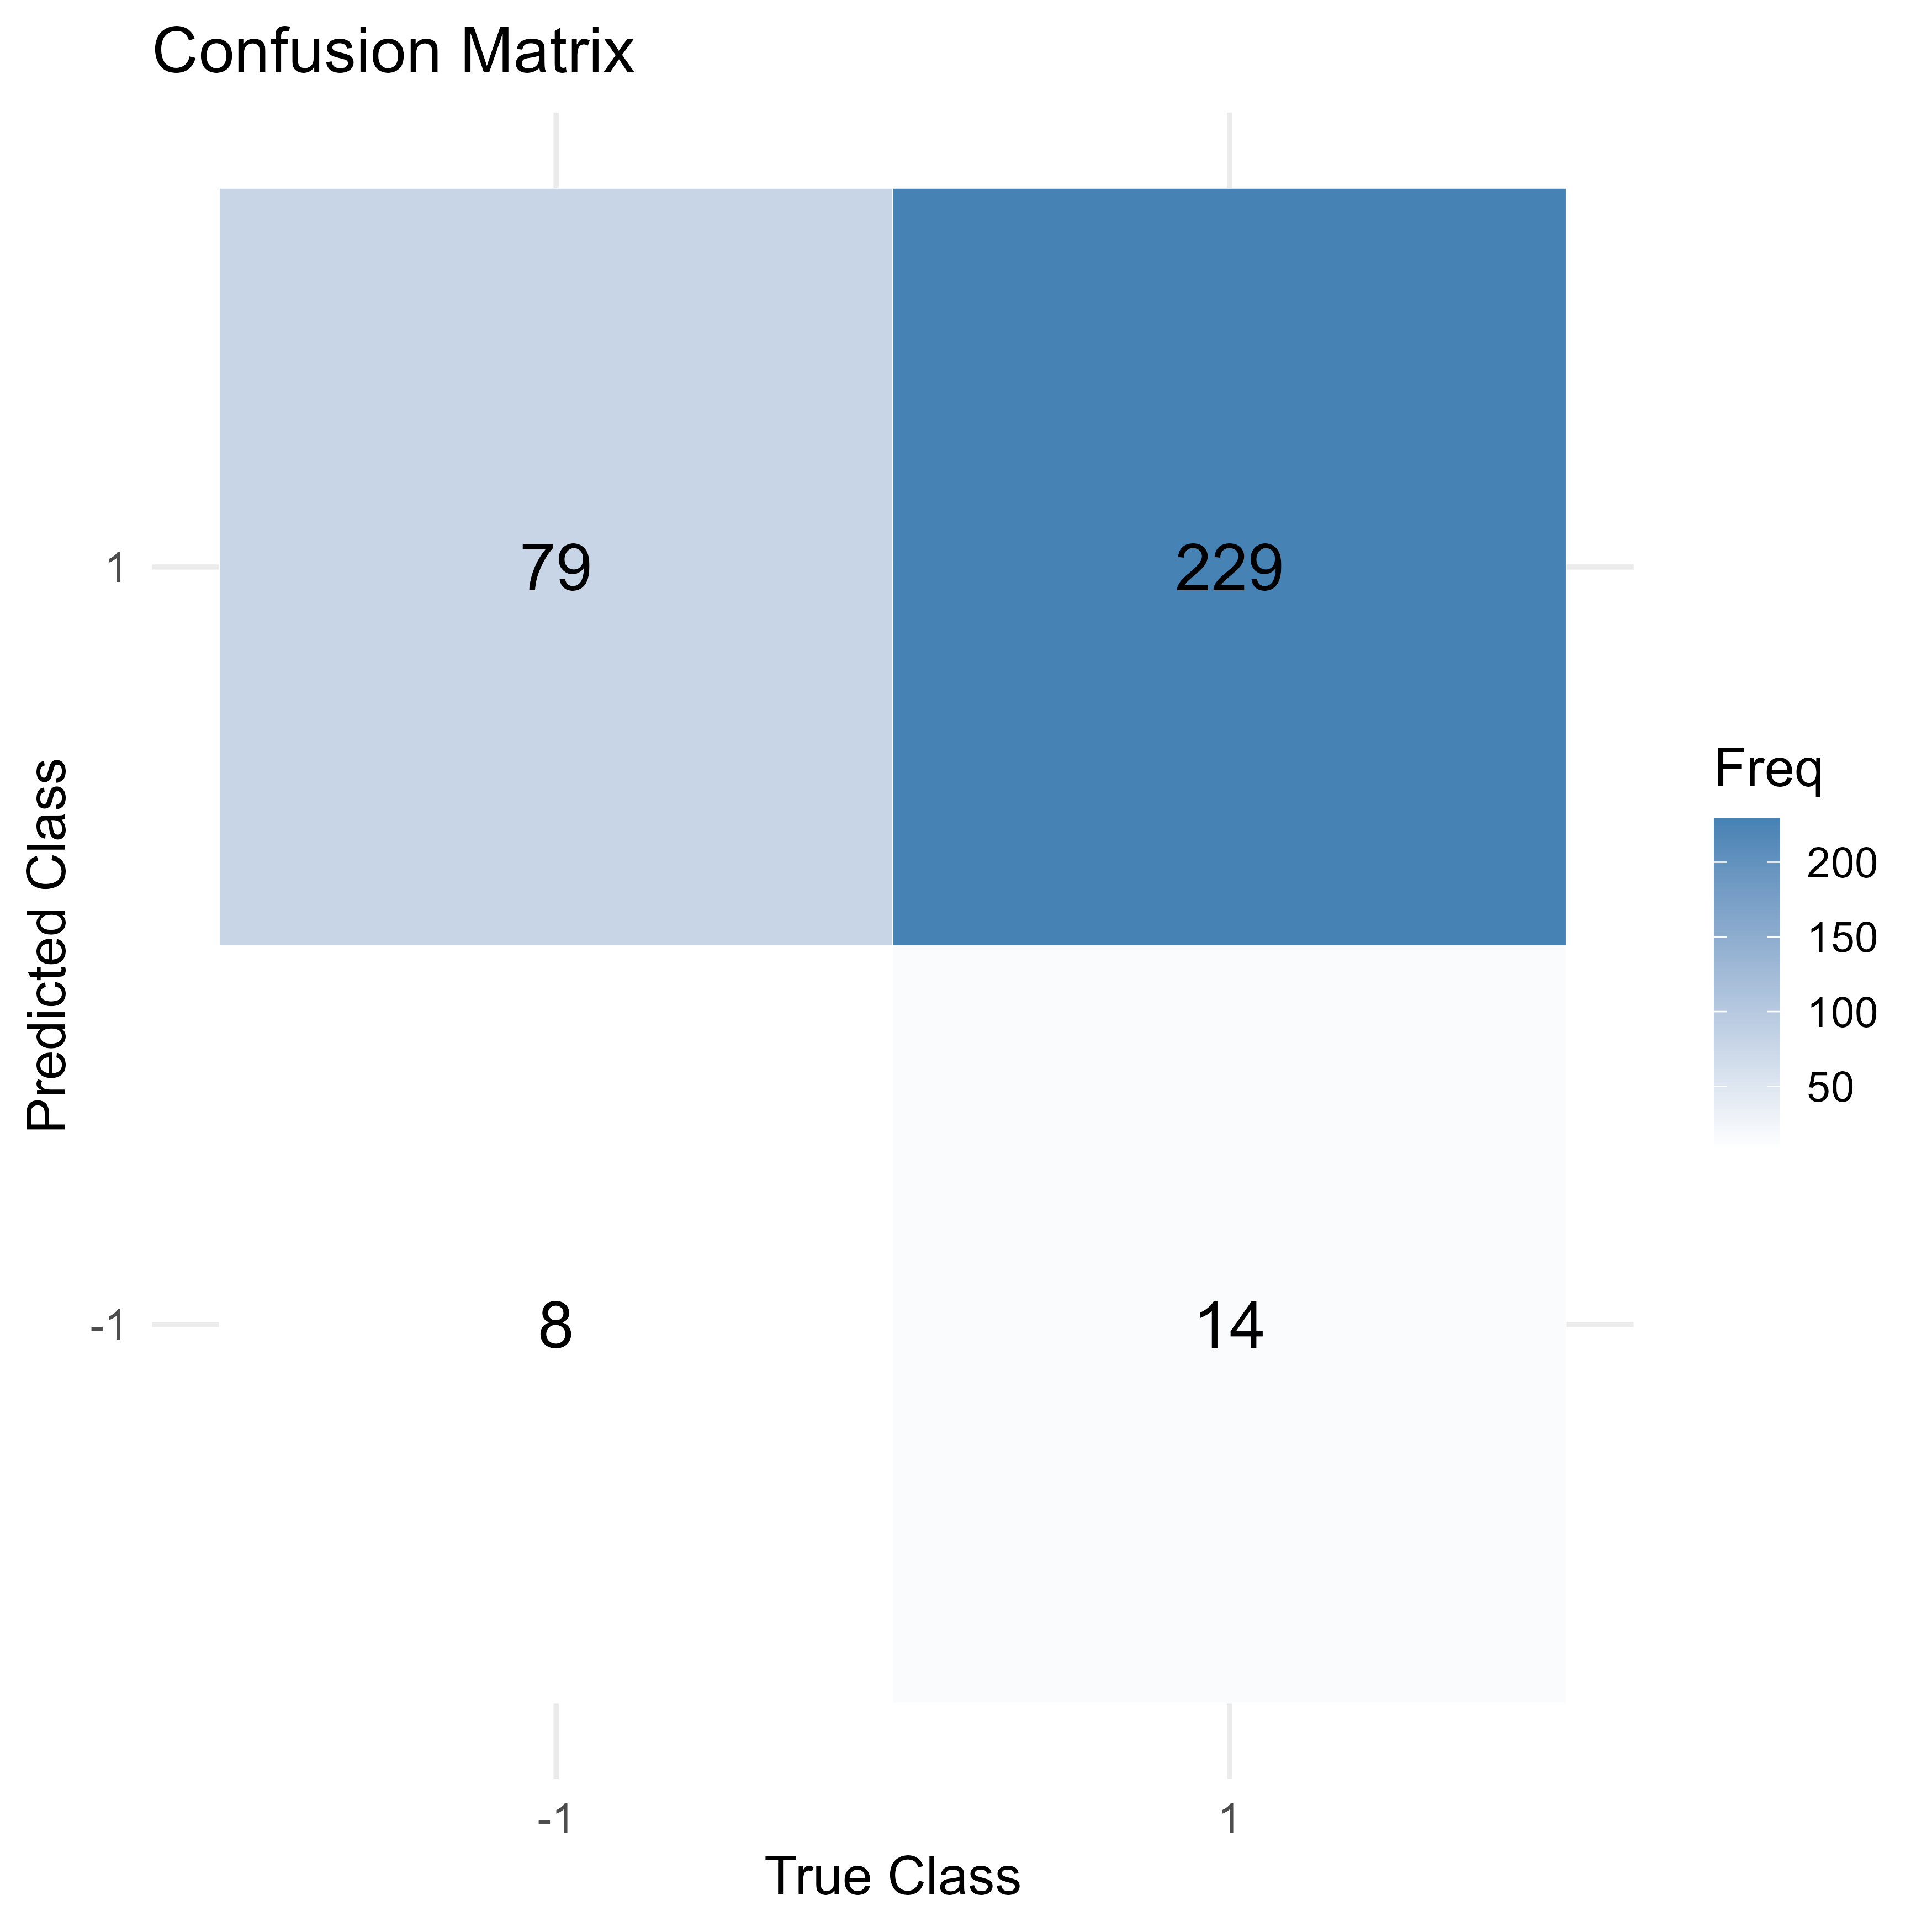
\includegraphics[scale = 0.3]{Pics/20}
		\caption{Confusion Matrix}
		\label{fig:20}
	\end{figure}
	\par Moreover, we compute F1 score of it, $0.147$, which means the predictive model has small ability to generalize with more situations. Then we turn to KNN with SMOTE.
	\subsubsection{KNN with SMOTE}
	\par With SMOTE, the KNN model's result also shown below.
			\begin{framed}
		\begin{verbatim}
		Confusion Matrix and Statistics
		Reference
		Prediction  -1   1
		-1  83 240
		1    4   3
		Accuracy : 0.2606          
		95% CI : (0.2141, 0.3115)                      
		\end{verbatim}
	\end{framed}
	The accuracy dropped to a bad situation, but with a higher $F1$ score: 0.404878.
	\subsection{Logistic Regression with SMOTE}
			\begin{framed}
		\begin{verbatim}
			Confusion Matrix and Statistics
			
			Reference
			Prediction  -1   1
			-1  58 164
			1   29  79
			
			Accuracy : 0.4152          
			95% CI : (0.3614, 0.4704)  
		\end{verbatim}
	\end{framed}
	\par As we can see, the accuracy gets higher, $41.52\%$, and the $F1$ score is $0.3754045$.
	\clearpage
	\subsection{XGBoost}
	\par Now we apply a new statistic method called XGBoost as our predictive model. After training, the results are
	\begin{framed}
		\begin{verbatim}
			Confusion Matrix and Statistics
			
			Reference
			Prediction  -1   1
			-1  35  65
			1   52 178
			
			Accuracy : 0.6455          
			95% CI : (0.5912, 0.6971)            
			
			F1 Score: 0.3743316      
		\end{verbatim}
	\end{framed}
	And the ROC curve is also shown below.
	\begin{figure}[htbp]
		\centering
		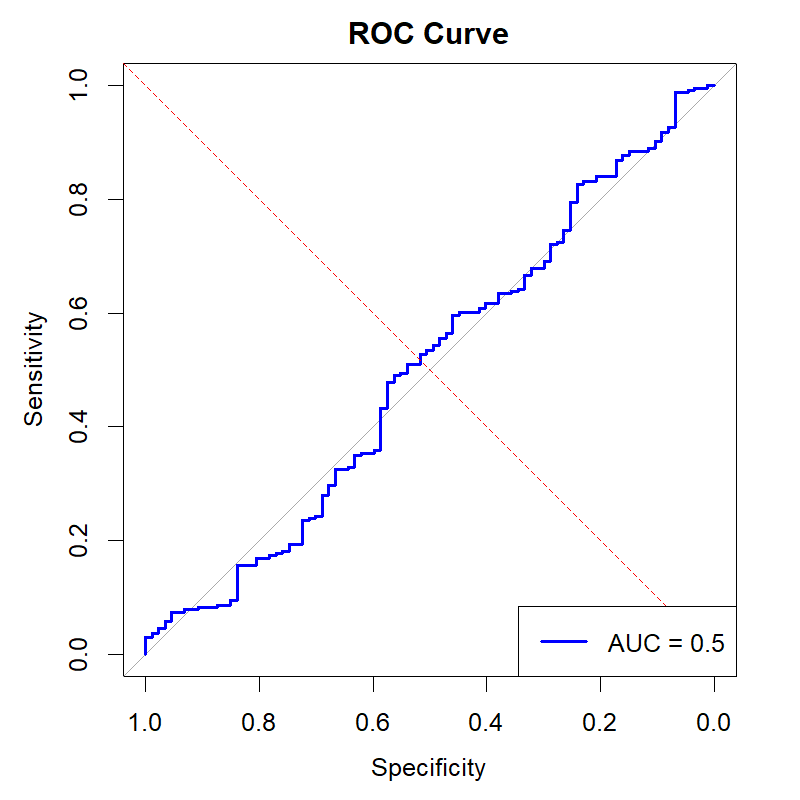
\includegraphics[scale = 0.5]{Pics/ROC_Curve}
		\caption{ROC Curve}
		\label{fig:roccurve}
	\end{figure}
	Although the accuracy is not the best, the F1 Score and the accuracy has a better performance all together, which have tried our best.
	\clearpage
	\section{The Predictive Model used in the Reference}
	\par In the reference \cite{ref1}, a \textbf{kernel method} was employed to analyze the firing patterns of individual neurons: The activity of neuron $ n $ at time $ t $ is modeled by the following equation:
	$$f_n(t) = \sum_{c} \sum_{t_s \in S_c} K_{c,n}(t - t_s) + \sum_{t_m \in M} \left( K_{m,n}(t - t_m) + D_m K_{D,n}(t - t_m) \right),$$
	where $ K_{c,n} $, $ K_{m,n} $, and $ K_{D,n} $ are kernel functions, $ S_c $ and $ M $ are sets of event times, and $ D_m $ is a scaling parameter.
	 \par This approach involved fitting a set of kernel functions to the neural activity, time-locked to specific task events such as \textbf{stimulus presentation} and\textbf{ movement onset}. The kernel functions were designed to capture variations in neural activity driven by different task variables, including visual stimuli, actions, and choices. Specifically, \textbf{six vision kernels} were fitted to represent the amplitude and timing of neural responses to different visual contrast levels, while\textbf{ a single action kernel} captured non-specific movement-related activity. Additionally,\textbf{ a choice kernel }was introduced to distinguish between left and right movement decisions. To determine the significance of these kernels, \textbf{a nested testing framework} was used, where models with and without specific kernels were compared to assess their predictive power. See more details in ref\cite{ref1}\cite{ref4}\cite{ref5}\cite{ref6}.
	\par This kernel-based approach provided a systematic way to identify how neurons encode task-relevant information, revealing the distributed nature of neural representations underlying behavior. The method's ability to capture both average activity patterns and trial-to-trial variability made it a powerful tool for understanding the functional roles of neurons in complex behavioral tasks.
	\par However, due to time constraints and the complexity involved, we are unable to delve deeper into this sophisticated model based on kernel fitting at this stage. Kernel fitting requires precise time-locked analysis of neuronal activity, as well as substantial computational resources and data preprocessing efforts, which are beyond the scope of our current research. Therefore, we were unable to replicate the full model presented in the paper. However, this does not hinder our understanding and application of the methodological principles outlined in the article. In the future, with more resources and time, we can further attempt to implement and validate this approach.
	\clearpage
	\section{Conclusion}
	\par This project aimed to develop a predictive model to classify behavioral outcomes (success or failure) based on neural activity and stimulus conditions in a visual discrimination task performed by mice. 
	\par Through a comprehensive analysis, we explored the structure of the data, integrated neural activity across sessions, and trained multiple machine learning models to predict trial outcomes.
	\par Key findings include the identification of significant variability in neural activity and task performance across sessions and mice, as highlighted by the box plot and the Kruskal-Wallis test. To address this variability, we employed data standardization, PCA for dimensionality reduction, and the Harmony algorithm for cross-session feature alignment. These steps ensured the robustness of our predictive models, which included LASSO, KNN, Logistic Regression, and XGBoost, with SMOTE used to mitigate class imbalance.
	\par The results demonstrate that neural activity in the visual cortex encodes information relevant to perceptual decision-making, and our models successfully captured these relationships. The integration of advanced statistical and machine learning techniques not only improved model performance but also provided insights into the neural mechanisms underlying decision-making. 
	\par This work contributes to the growing field of neuroscience by offering a methodological framework for analyzing high-dimensional neural datasets and advancing our understanding of how sensory input and neural dynamics translate into behavior. Future research could explore additional neural regions, refine model architectures, and investigate the generalizability of these findings to other decision-making tasks.
	\clearpage
	\begin{thebibliography}{99} 
		\bibitem{ref1} Steinmetz N A, Zatka-Haas P, Carandini M, et al. Distributed coding of choice, action and engagement across the mouse brain[J]. Nature, 2019, 576(7786): 266-273.
		\bibitem{ref2}  Brain diagrams were derived from the Allen Mouse Brain Common Coordinate Framework (version 3 (2017); downloaded from http://download.alleninstitute.org/informatics-archive/current-release/mouse\_ccf/)
		\bibitem{ref3} Jun, J. J. et al. Fully integrated silicon probes for high-density recording of neural activity. Nature 551, 232–236 (2017).
		\bibitem{ref4} Park, I. M., Meister, M. L. R., Huk, A. C. \& Pillow, J. W. Encoding and decoding in parietal cortex during sensorimotor decision-making. Nat. Neurosci. 17, 1395–1403 (2014).
		\bibitem{ref5} Ashe, J. \& Georgopoulos, A. P. Movement parameters and neural activity in motor cortex and area 5. Cereb. Cortex 4, 590–600 (1994).
		\bibitem{ref6} Paninski, L., Shoham, S., Fellows, M. R., Hatsopoulos, N. G. \& Donoghue, J. P. Superlinear population encoding of dynamic hand trajectory in primary motor cortex. J. Neurosci. 24, 8551–8561 (2004).
	\end{thebibliography}
	\clearpage
	\appendix
	\section{Tables}
	\subsection{Session-Wise Summary Table}
	\begin{table}[htbp]
		\centering
		\begin{adjustbox}{width=\textwidth}  % 调整表格宽度以适应页面
			\begin{tabular}{llrrr}
				\toprule
				\textbf{session\_id} & \textbf{mouse} & \textbf{n\_neurons} & \textbf{n\_trials} & \textbf{success\_rate} \\
				\midrule
				2016-12-14 & Cori       &  734 & 114 & 0.6053 \\
				2016-12-17 & Cori       & 1070 & 251 & 0.6335 \\
				2016-12-18 & Cori       &  619 & 228 & 0.6623 \\
				2017-11-01 & Forssmann  & 1769 & 249 & 0.6667 \\
				2017-11-02 & Forssmann  & 1077 & 254 & 0.6614 \\
				2017-11-04 & Forssmann  & 1169 & 290 & 0.7414 \\
				2017-11-05 & Forssmann  &  584 & 252 & 0.6706 \\
				2017-06-15 & Hench      & 1157 & 250 & 0.6440 \\
				2017-06-16 & Hench      &  788 & 372 & 0.6855 \\
				2017-06-17 & Hench      & 1172 & 447 & 0.6197 \\
				2017-06-18 & Hench      &  857 & 342 & 0.7953 \\
				2017-12-05 & Lederberg  &  698 & 340 & 0.7382 \\
				2017-12-06 & Lederberg  &  983 & 300 & 0.7967 \\
				2017-12-07 & Lederberg  &  756 & 268 & 0.6940 \\
				2017-12-08 & Lederberg  &  743 & 404 & 0.7649 \\
				2017-12-09 & Lederberg  &  474 & 280 & 0.7179 \\
				2017-12-10 & Lederberg  &  565 & 224 & 0.8304 \\
				2017-12-11 & Lederberg  & 1090 & 216 & 0.8056 \\
				\bottomrule
			\end{tabular}
		\end{adjustbox}
		\caption{Session-wise Summary}
		\label{tab:session_summary}
	\end{table}
\end{document}